\chapter{Requirements Specification and Analysis}\label{ch:3}

This chapter specifies what the \emph{AI Legal Advisor and Analyzer} must do and how well it must do it, then analyses the requirements through use cases, sequence diagrams, a domain model and user-interface prototypes. All requirements describe the planned system. None of them should be read as already implemented.

The system has three portals: the \textbf{User portal} for citizens, the \textbf{Lawyer portal} and the \textbf{Admin portal}. It is built on the architecture defined in Chapter 1:

\begin{itemize}
  \item \textbf{Presentation layer:} React / Next.js.
  \item \textbf{Application layer:} a Python FastAPI backend with REST APIs.
  \item \textbf{Data layer:} MongoDB for application data, a file store for uploaded documents, and the Qdrant vector database for legal-text embeddings.
  \item \textbf{AI services:} Sentence Transformers for embeddings, an open-source large language model (LLM) for grounded generation, PyMuPDF for PDF text extraction, and an OCR engine for scanned documents and images.
\end{itemize}

The legal scope is limited to \textbf{property disputes} and \textbf{family disputes} under Pakistani law.

Each requirement has a unique identifier and a priority:

\begin{itemize}
  \item \textbf{High:} essential for the final demonstration.
  \item \textbf{Medium:} planned and expected.
  \item \textbf{Low:} delivered if time permits.
\end{itemize}

\needspace{12\baselineskip}
\section{Functional Requirements}

\subsection{User Portal (Citizen)}

\begin{longtable}{|L{1.68cm}|L{2.24cm}|L{8.39cm}|L{1.70cm}|}
\caption{Functional requirements of the User portal}\label{tab:3.1}\\
\hline\headrow \thd{ID} & \thd{Requirement} & \thd{Description} & \thd{Priority} \\ \hline
\endfirsthead
\hline\headrow \thd{ID} & \thd{Requirement} & \thd{Description} & \thd{Priority} \\ \hline
\endhead
\hline\endlastfoot
\multicolumn{4}{|l|}{\cellcolor{rowtint}\textbf{Authentication and profile}} \\ \hline
UFR-01 & Register account & The system shall allow a citizen to register with full name, email, mobile number and password. The email address shall be verified before the account is activated. & High \\ \hline
UFR-02 & Log in and log out & The system shall authenticate users with email and password and issue a signed access token for subsequent requests. & High \\ \hline
UFR-03 & Reset password & The system shall allow a user to reset a forgotten password through a time-limited link sent by email. & Medium \\ \hline
UFR-04 & Manage profile & The system shall allow a user to view and update personal details (name, phone, city, preferred language) and change the password. & Medium \\ \hline
UFR-05 & Delete account & The system shall allow a user to request deletion of the account and personal case data, subject to the retention rules in NFR-PRV-04. & Low \\ \hline
\multicolumn{4}{|l|}{\cellcolor{rowtint}\textbf{AI legal assistance}} \\ \hline
UFR-06 & Describe a legal problem & The system shall allow a user to describe a problem in free text. This starts an AI chat session linked to a new or existing case. & High \\ \hline
UFR-07 & Detect legal area and topic & The system shall classify the problem into a legal area (property or family) and a topic (e.g. tenancy and eviction, inheritance, khula, maintenance, custody), and shall let the user correct the classification. & High \\ \hline
UFR-08 & Ask follow-up questions & The system shall identify facts that are missing for the detected topic and ask the user only the follow-up questions needed to fill them, one at a time, before giving guidance. & High \\ \hline
UFR-09 & Retrieve relevant law & The system shall convert the clarified case into a query embedding (Sentence Transformers) and retrieve the top-k most relevant law sections and case references from Qdrant, filtered by legal area. & High \\ \hline
UFR-10 & Generate grounded guidance & The system shall send the open-source LLM a prompt containing only the retrieved sections, the case facts and an instruction to answer only from those sections, and shall present the answer in plain language. & High \\ \hline
UFR-11 & Cite sources & The system shall attach a citation (law or judgment title, section or paragraph, and quoted text) to every statement of the guidance and display a sources list. & High \\ \hline
UFR-12 & Verify citations & The system shall check that every citation in a generated answer refers to a retrieved source before showing the answer. An answer that fails the check shall be regenerated or withheld. & High \\ \hline
UFR-13 & Handle unsupported questions & When no verified source is sufficiently relevant, or the question is outside property and family law, the system shall say so and recommend consulting a verified lawyer instead of producing an answer. & High \\ \hline
UFR-14 & Show disclaimer & Every guidance screen shall state that the platform provides legal information and does not replace a qualified lawyer. & High \\ \hline
UFR-15 & Continue the conversation & The system shall let the user ask further questions in the same chat session, reusing the stored case facts and history. & Medium \\ \hline
\multicolumn{4}{|l|}{\cellcolor{rowtint}\textbf{Case management and documents}} \\ \hline
UFR-16 & Create and manage cases & The system shall allow a user to create, rename, view and close cases. Each case stores its legal area, topic, facts, chat sessions, guidance, documents and status. & High \\ \hline
UFR-17 & Upload documents & The system shall allow a user to upload PDF, JPG and PNG files (e.g. rent agreement, notice, nikah nama, receipts) to a case. & High \\ \hline
UFR-18 & Extract document text & The system shall extract text with PyMuPDF for digital PDFs and with OCR for scanned files and images, and shall record the extraction method. & High \\ \hline
UFR-19 & Identify key clauses & The system shall identify key clauses in uploaded agreements and notices (e.g. parties, rent, term, notice period, dower amount) and show them to the user. & Medium \\ \hline
UFR-20 & Generate evidence checklist & The system shall generate a case-specific checklist of documents and evidence to prepare, and shall mark an item as available when a matching document is uploaded. & High \\ \hline
UFR-21 & Generate case summary & The system shall generate a short case summary (facts, issues, relevant law, available evidence) that can be shared with a lawyer. & Medium \\ \hline
\multicolumn{4}{|l|}{\cellcolor{rowtint}\textbf{Lawyer search and consultations}} \\ \hline
UFR-22 & Search lawyers & The system shall allow a user to search verified lawyers and filter by specialisation, city, fee range, years of experience, language and rating. & High \\ \hline
UFR-23 & View public lawyer profile & The system shall display a public, professional-network-style profile for each verified lawyer: photo, headline, about section, practice areas, experience history, education and qualifications, bar enrolment details, languages, fee range, rating and reviews. & High \\ \hline
UFR-24 & Request consultation & The system shall allow a user to send a consultation request to a lawyer, stating the preferred mode (online or in person), preferred time and a message. & High \\ \hline
UFR-25 & Share case with consent & The system shall share a case with a lawyer only after the user explicitly agrees, and shall show exactly which items (summary, guidance, documents, contact details) will be shared. & High \\ \hline
UFR-26 & Revoke sharing & The system shall allow a user to stop sharing a case with a lawyer at any time. & Medium \\ \hline
UFR-27 & Message lawyer & The system shall provide in-app messaging between the user and the lawyer within an accepted consultation. & Medium \\ \hline
UFR-28 & Rate and review & The system shall allow a user to rate (1-5) and review a lawyer after a consultation is marked completed. & Low \\ \hline
\multicolumn{4}{|l|}{\cellcolor{rowtint}\textbf{Case tracking and notifications}} \\ \hline
UFR-29 & Track case progress & The system shall show a timeline of each case: creation, clarification, guidance, documents, consultations and every status update, until the case is resolved or closed. & High \\ \hline
UFR-30 & Receive notifications & The system shall notify the user in-app, and optionally by email, when a lawyer responds, a consultation is scheduled or the case status changes. & Medium \\
\end{longtable}

\subsection{Lawyer Portal}

\begin{longtable}{|L{1.66cm}|L{2.35cm}|L{8.30cm}|L{1.70cm}|}
\caption{Functional requirements of the Lawyer portal}\label{tab:3.2}\\
\hline\headrow \thd{ID} & \thd{Requirement} & \thd{Description} & \thd{Priority} \\ \hline
\endfirsthead
\hline\headrow \thd{ID} & \thd{Requirement} & \thd{Description} & \thd{Priority} \\ \hline
\endhead
\hline\endlastfoot
LFR-01 & Register as lawyer & The system shall allow a lawyer to register with personal details, bar enrolment/licence number, issuing bar council and a copy of the licence, and shall create the account in a \emph{pending verification} state. & High \\ \hline
LFR-02 & Log in and log out & The system shall authenticate lawyers in the same way as users, with access restricted to Lawyer-portal functions. & High \\ \hline
LFR-03 & Build public profile & The system shall allow a lawyer to create and edit a public profile: headline, about, practice areas (property, family and sub-topics), experience entries, education and qualifications, languages, city, office address, fee range and profile photo. & High \\ \hline
LFR-04 & Profile visibility & The system shall publish a lawyer's profile in the directory only after an administrator has verified the lawyer, and shall show a ``Verified'' badge. & High \\ \hline
LFR-05 & Manage availability & The system shall allow a lawyer to set availability for consultations and to pause new requests. & Medium \\ \hline
LFR-06 & View consultation requests & The system shall list incoming consultation requests with the case title, legal area, case summary and evidence-checklist progress shared by the user. & High \\ \hline
LFR-07 & Respond to requests & The system shall allow a lawyer to accept, decline or propose another time for a consultation request, optionally with a message. & High \\ \hline
LFR-08 & Access shared case & The system shall give a lawyer read-only access to the case items the user consented to share, for as long as sharing is active. & High \\ \hline
LFR-09 & Message user & The system shall allow a lawyer to exchange messages with the user within an accepted consultation. & Medium \\ \hline
LFR-10 & Post case updates & The system shall allow a lawyer to post status updates and notes on an accepted case; these appear on the user's case timeline. & High \\ \hline
LFR-11 & Complete consultation & The system shall allow a lawyer to mark a consultation as completed, which enables the user to leave a review. & Medium \\ \hline
LFR-12 & View dashboard & The system shall show the lawyer counts of new requests, active cases, completed consultations and average rating. & Medium \\
\end{longtable}

\subsection{Admin Portal}

\begin{longtable}{|L{1.62cm}|L{2.57cm}|L{8.12cm}|L{1.70cm}|}
\caption{Functional requirements of the Admin portal}\label{tab:3.3}\\
\hline\headrow \thd{ID} & \thd{Requirement} & \thd{Description} & \thd{Priority} \\ \hline
\endfirsthead
\hline\headrow \thd{ID} & \thd{Requirement} & \thd{Description} & \thd{Priority} \\ \hline
\endhead
\hline\endlastfoot
AFR-01 & Secure admin login & The system shall allow only accounts with the administrator role to access the Admin portal. & High \\ \hline
AFR-02 & Verify lawyers & The system shall list pending lawyer registrations with submitted licence documents and allow an administrator to approve or reject each, recording the reason and the administrator's identity. & High \\ \hline
AFR-03 & Manage users and lawyers & The system shall allow an administrator to search, view, suspend, reactivate and remove user and lawyer accounts. & High \\ \hline
AFR-04 & Moderate profiles and reviews & The system shall allow an administrator to review and remove inappropriate profile content and reviews, including items reported by users. & Medium \\ \hline
AFR-05 & Manage legal sources & The system shall allow an administrator to add a legal source (statute, ordinance, rules or judgment) with metadata (title, type, year, legal area, official URL) and mark it as verified. & High \\ \hline
AFR-06 & Index legal sources & The system shall extract the text of a new source (PyMuPDF/OCR), split it into section-wise chunks with metadata, generate embeddings and store them in Qdrant. Only verified sources shall be searchable. & High \\ \hline
AFR-07 & Update or retire sources & The system shall allow an administrator to re-index an amended source or retire an outdated one so that it is no longer retrieved. & Medium \\ \hline
AFR-08 & Monitor platform activity & The system shall show a dashboard with counts of users, verified lawyers, open cases, consultations, indexed sections and guidance requests, and the rate of withheld (unsupported) answers. & Medium \\ \hline
AFR-09 & View audit log & The system shall record administrative actions (verification, suspension, source changes) in an audit log that administrators can view and filter. & Medium \\
\end{longtable}

\section{Non-Functional Requirements}

The following targets are design goals. They will be measured during testing and evaluation and may be adjusted to the capacity of the deployment server.

\begin{longtable}{|L{1.70cm}|L{1.70cm}|L{7.76cm}|L{2.85cm}|}
\caption{Non-functional requirements}\label{tab:3.4}\\
\hline\headrow \thd{ID} & \thd{Category} & \thd{Requirement} & \thd{Measure / verification} \\ \hline
\endfirsthead
\hline\headrow \thd{ID} & \thd{Category} & \thd{Requirement} & \thd{Measure / verification} \\ \hline
\endhead
\hline\endlastfoot
NFR-SEC-01 & Security & Passwords shall be stored only as salted hashes (bcrypt or Argon2). & Code review; database inspection \\ \hline
NFR-SEC-02 & Security & All client-server traffic shall use HTTPS. APIs shall require a signed access token, and every endpoint shall check the caller's role (user, lawyer, admin). & Penetration and access-control tests \\ \hline
NFR-SEC-03 & Security & Uploaded files shall be checked for type and size (e.g. at most 10 MB) and stored outside the public web root. & Upload tests with invalid files \\ \hline
NFR-SEC-04 & Security & Text from user messages and uploaded documents shall be treated as data, never as instructions to the LLM, to resist prompt injection. & Adversarial prompt tests \\ \hline
NFR-PRF-01 & Performance & Non-AI pages shall load within 2 seconds for 95\% of requests under normal load. & Load testing \\ \hline
NFR-PRF-02 & Performance & Retrieval from Qdrant shall return results within 1 second. A complete guidance answer shall be produced within 30 seconds for 90\% of requests, with a progress indicator shown meanwhile. & Timed test runs \\ \hline
NFR-PRF-03 & Performance & OCR of a single-page image shall complete within 15 seconds. & Timed test runs \\ \hline
NFR-REL-01 & Reliability & If the LLM, OCR or vector service fails, the system shall show a clear error and preserve the case, chat history and uploaded files without loss. & Fault-injection tests \\ \hline
NFR-REL-02 & Reliability & Long-running tasks (OCR, indexing) shall run asynchronously and be retried on failure. & Integration tests \\ \hline
NFR-REL-03 & Reliability & The deployed system shall target 99\% availability during the evaluation period, with regular database backups. & Uptime monitoring \\ \hline
NFR-SCL-01 & Scalability & The frontend, backend, MongoDB and Qdrant shall run as separate components that can be scaled or replaced independently. & Architecture review \\ \hline
NFR-SCL-02 & Scalability & New legal areas shall be addable by ingesting verified sources, without changing the RAG pipeline code. & Ingestion test with a new source \\ \hline
NFR-USA-01 & Usability & A first-time user shall be able to create a case and read guidance without assistance. & Task-based usability test \\ \hline
NFR-USA-02 & Usability & The system shall achieve a System Usability Scale (SUS) score of at least 68 \cite{r29}, \cite{r30}. & SUS questionnaire \\ \hline
NFR-USA-03 & Usability & Guidance shall use plain language, explain unavoidable legal terms, and the interface shall be responsive on desktop and mobile. & Expert review; device testing \\ \hline
NFR-MNT-01 & Maintainability & The code shall be version-controlled with Git, follow a layered structure (routes, services, repositories), and expose documented REST APIs (OpenAPI). & Code review \\ \hline
NFR-MNT-02 & Maintainability & Prompts, retrieval parameters (e.g. top-k) and model names shall be configurable without code changes. & Configuration review \\ \hline
NFR-PRV-01 & Data privacy & A case shall be visible only to its owner, to lawyers with active consent, and to administrators for moderation. & Access-control tests \\ \hline
NFR-PRV-02 & Data privacy & A lawyer's public profile shall not expose personal contact details until a consultation is accepted. & UI and API review \\ \hline
NFR-PRV-03 & Data privacy & Case text and documents shall not be used to train models and shall not be sent to third-party services without the user's consent. & Configuration review \\ \hline
NFR-PRV-04 & Data privacy & Deleted accounts and cases shall be removed or anonymised, except records that must be kept for audit. & Deletion tests \\ \hline
NFR-ACC-01 & Accuracy & Every statement in a guidance answer shall cite a retrieved, verified source (100\% citation coverage on the test set). & Automated citation check \\ \hline
NFR-ACC-02 & Accuracy & On a test set of property and family questions, the RAG system shall score higher than a standard LLM baseline on the defined quality measures (correctness, groundedness, citation accuracy). & Comparative evaluation \\ \hline
NFR-ACC-03 & Accuracy & For out-of-scope or unsupported questions, the system shall decline instead of answering. & Test set of negative cases \\ \hline
NFR-ACC-04 & Accuracy & Document text extraction shall be checked against manually transcribed samples to measure OCR quality. & Character-level comparison on samples \\
\end{longtable}

\section{System Use Case Modeling}

The system has three primary actors and two secondary (supporting) actors:

\begin{center}
\begin{tabular}{|L{2.12cm}|L{1.76cm}|L{10.59cm}|}
\hline\headrow \thd{Actor} & \thd{Type} & \thd{Role} \\ \hline
\textbf{User (Citizen)} & Primary & Describes legal problems, receives grounded guidance, uploads evidence, finds lawyers, requests consultations and tracks cases. \\ \hline
\textbf{Lawyer} & Primary & Maintains a public profile, handles consultation requests, accesses shared cases and posts case updates. \\ \hline
\textbf{Admin} & Primary & Verifies lawyers, manages accounts and legal sources, and monitors platform activity. \\ \hline
\textbf{AI Services} & Secondary (system) & Embedding model, Qdrant retrieval, open-source LLM and OCR that support guidance and document analysis. \\ \hline
\textbf{Email Service} & Secondary (external) & Sends verification, password-reset and notification emails. \\ \hline
\end{tabular}
\end{center}

Mermaid has no native UML use-case notation. Figures~\ref{fig:3.1} to~\ref{fig:3.3} therefore use flowchart nodes in the conventional style: actors outside the system boundary, use cases as rounded nodes inside it, and dashed arrows for \texttt{<{}<include>{}>} and \texttt{<{}<extend>{}>} relationships.

% Mermaid source:
% flowchart LR
%     User["User (Citizen)"]
%     AI["AI Services"]
%     subgraph SYS["AI Legal Advisor and Analyzer: User Portal"]
%         UC1(["UC-01 Register and Authenticate"])
%         UC2(["UC-02 Create Case and Clarify Facts"])
%         UC3(["UC-03 Obtain AI Legal Guidance"])
%         UC4(["UC-04 Upload and Analyse Documents"])
%         UC5(["UC-05 Search Lawyers and View Profile"])
%         UC6(["UC-06 Request Consultation and Share Case"])
%         UC7(["UC-07 Track Case Progress"])
%         UCv(["Verify Citations"])
%         UCck(["Generate Evidence Checklist"])
%         UCrv(["Rate and Review Lawyer"])
%     end
%     User --- UC1
%     User --- UC2
%     User --- UC3
%     User --- UC4
%     User --- UC5
%     User --- UC6
%     User --- UC7
%     UC3 -. "include" .-> UCv
%     UC4 -. "include" .-> UCck
%     UC3 -. "include" .-> UC2
%     UCrv -. "extend" .-> UC7
%     UC3 --- AI
%     UC4 --- AI
\begin{figure}[H]\centering
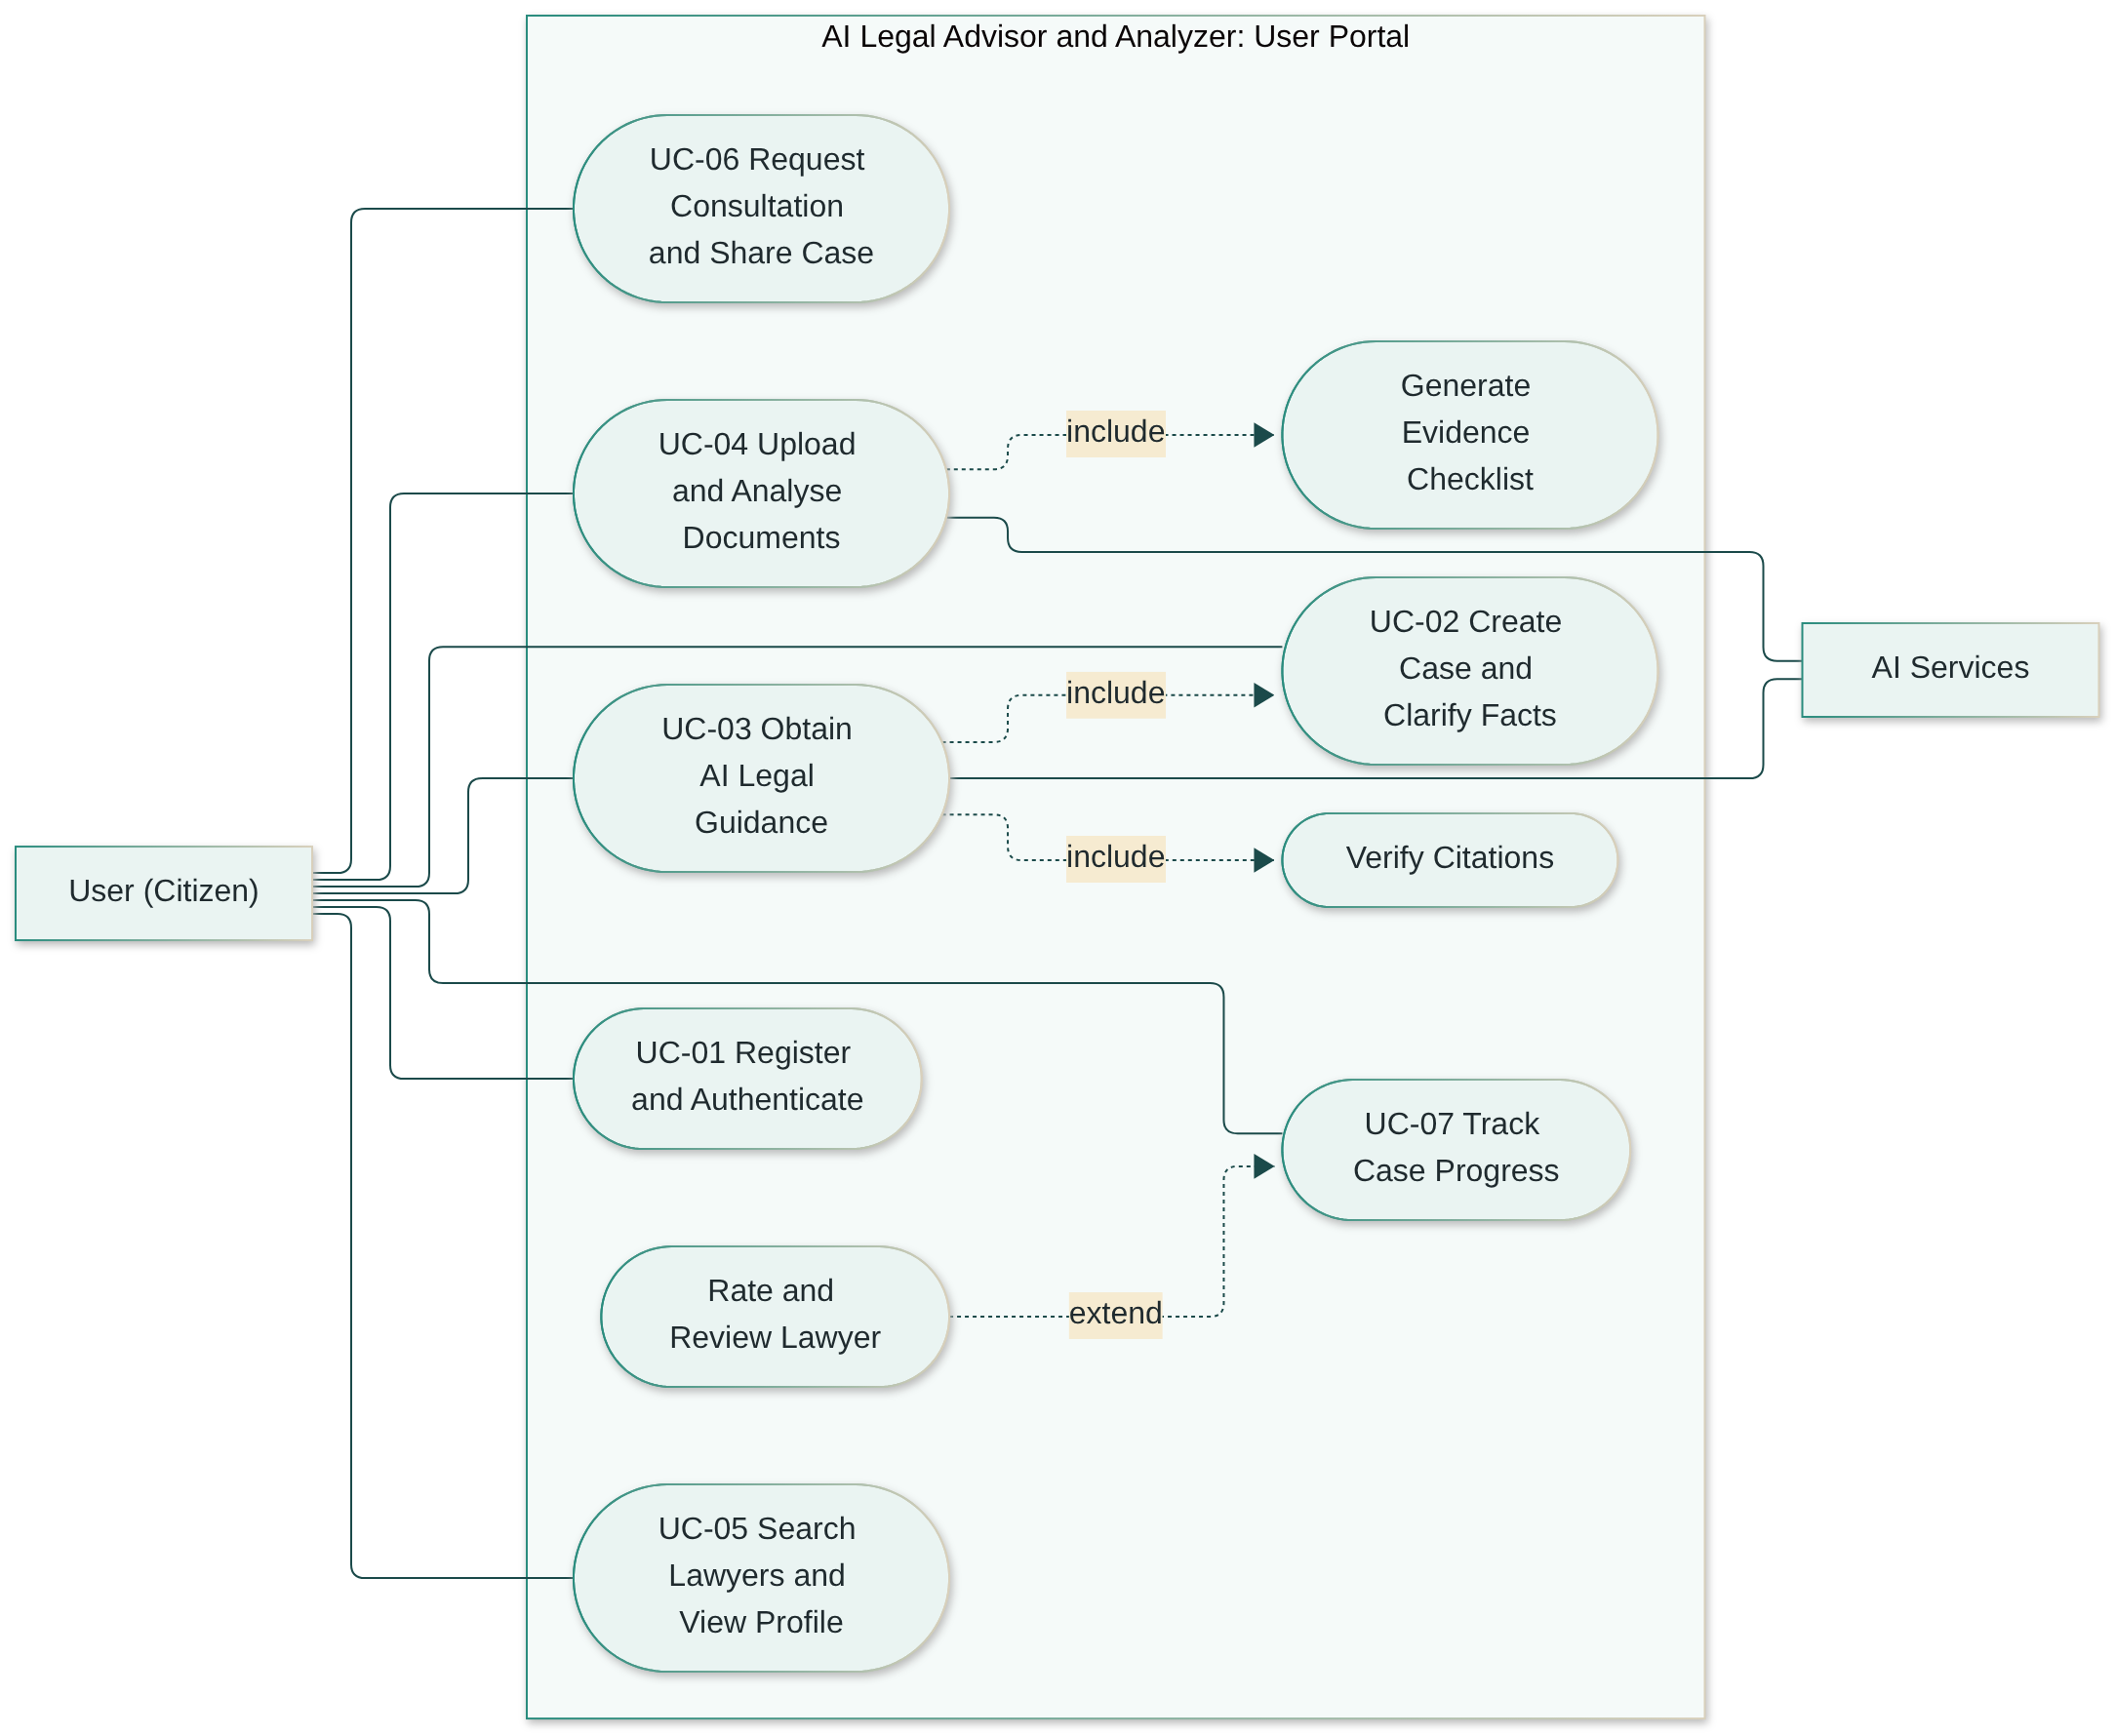
\includegraphics[width=\textwidth,height=0.62\textheight,keepaspectratio]{figures/uc_user.png}
\caption{Use case diagram, User portal}\label{fig:3.1}
\end{figure}

% Mermaid source:
% flowchart LR
%     Lawyer["Lawyer"]
%     subgraph SYS["AI Legal Advisor and Analyzer: Lawyer Portal"]
%         UC1(["UC-01 Register and Authenticate"])
%         UC8(["UC-08 Manage Public Profile and Verification Request"])
%         UC9(["UC-09 Handle Consultation Requests"])
%         UC9b(["View Shared Case"])
%         UC9c(["Post Case Status Update"])
%         UC9d(["Message User"])
%     end
%     Lawyer --- UC1
%     Lawyer --- UC8
%     Lawyer --- UC9
%     UC9 -. "include" .-> UC9b
%     UC9c -. "extend" .-> UC9
%     UC9d -. "extend" .-> UC9
\begin{figure}[H]\centering
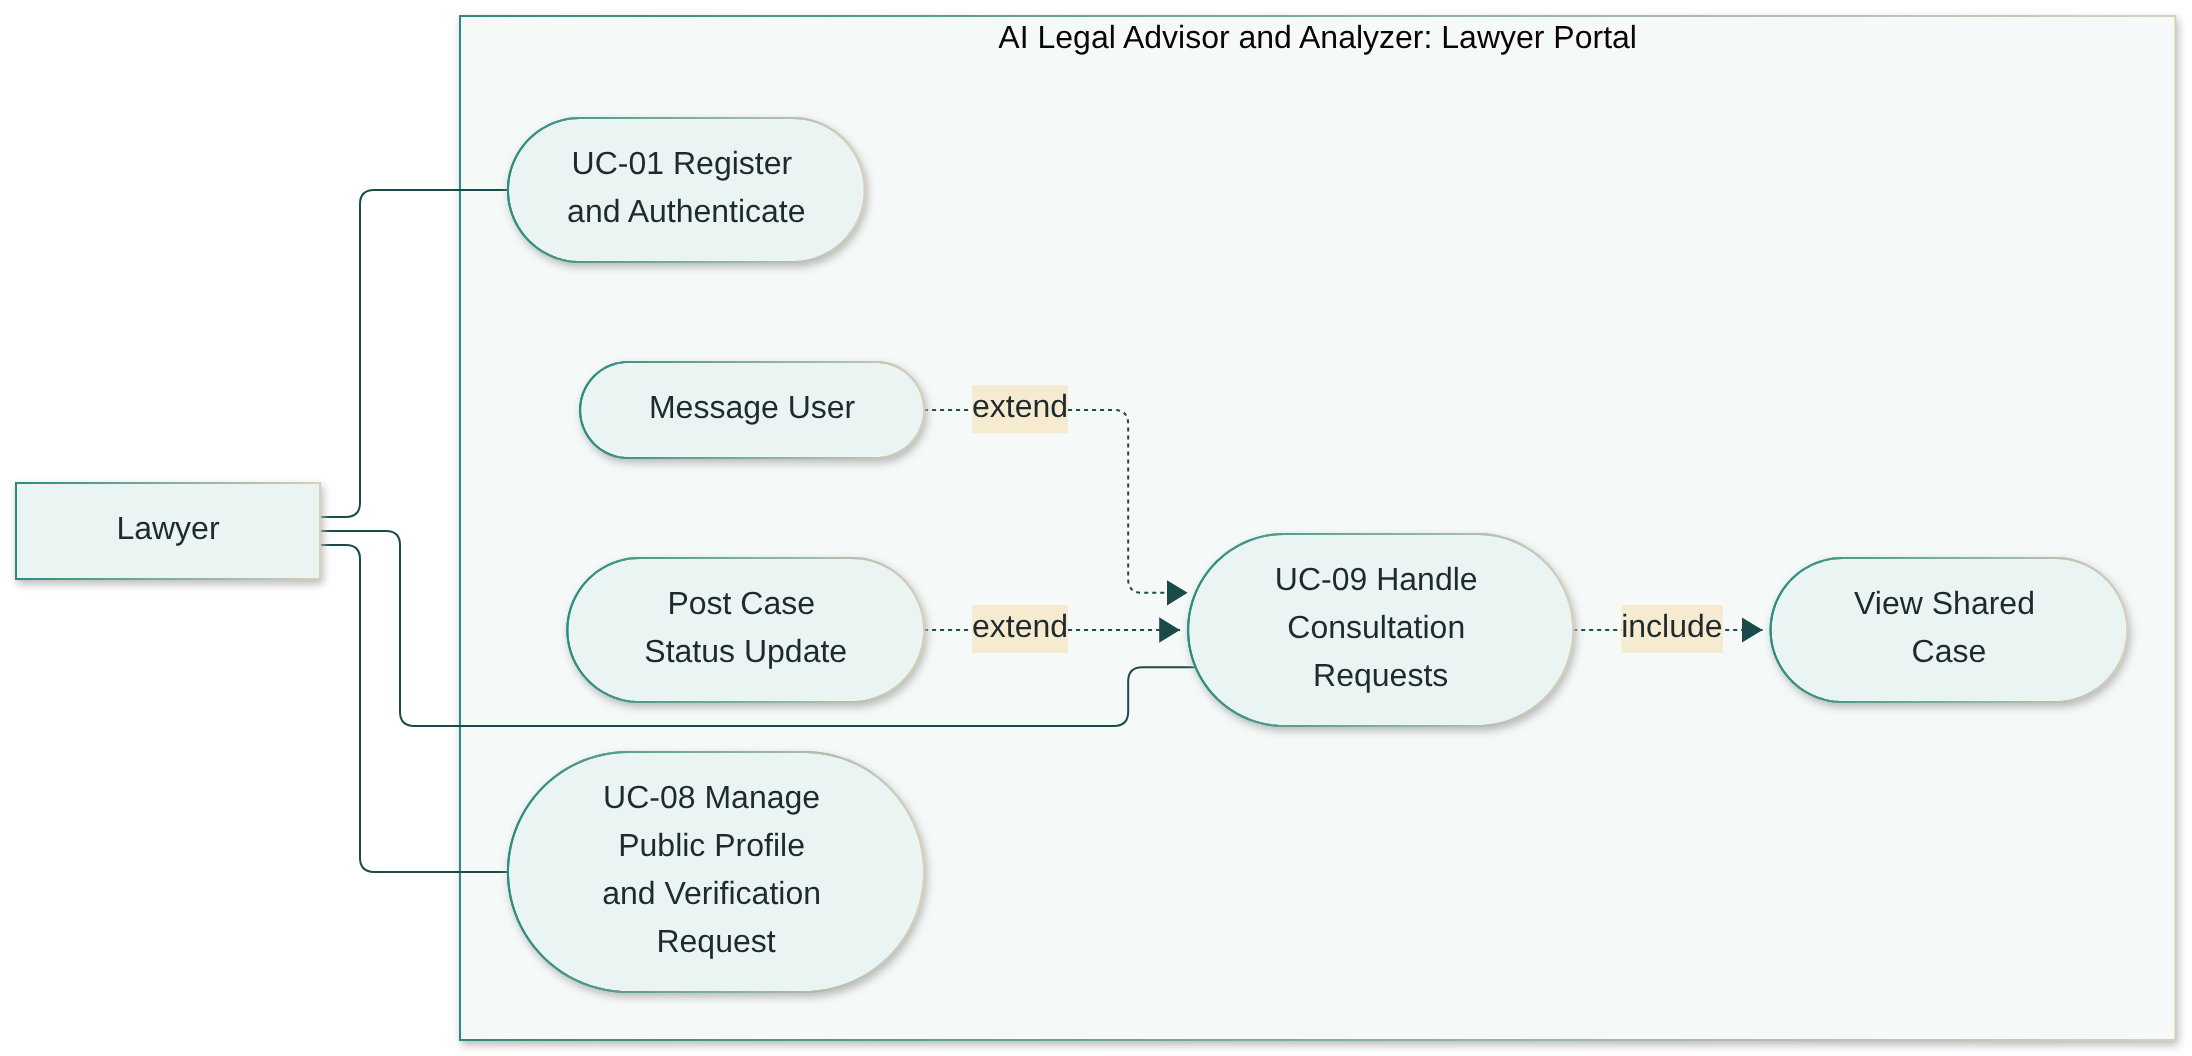
\includegraphics[width=\textwidth,height=0.62\textheight,keepaspectratio]{figures/uc_lawyer.png}
\caption{Use case diagram, Lawyer portal}\label{fig:3.2}
\end{figure}

% Mermaid source:
% flowchart LR
%     Admin["Admin"]
%     AI["AI Services"]
%     subgraph SYS["AI Legal Advisor and Analyzer: Admin Portal"]
%         UC1(["UC-01 Authenticate"])
%         UC10(["UC-10 Verify Lawyer Accounts"])
%         UC11(["UC-11 Manage Legal Knowledge Base"])
%         UC12(["UC-12 Manage Users and Monitor Activity"])
%         UC11b(["Index Source into Qdrant"])
%         UC12b(["Moderate Profiles and Reviews"])
%         UC12c(["View Audit Log"])
%     end
%     Admin --- UC1
%     Admin --- UC10
%     Admin --- UC11
%     Admin --- UC12
%     UC11 -. "include" .-> UC11b
%     UC12b -. "extend" .-> UC12
%     UC12c -. "extend" .-> UC12
%     UC11b --- AI
\begin{figure}[H]\centering
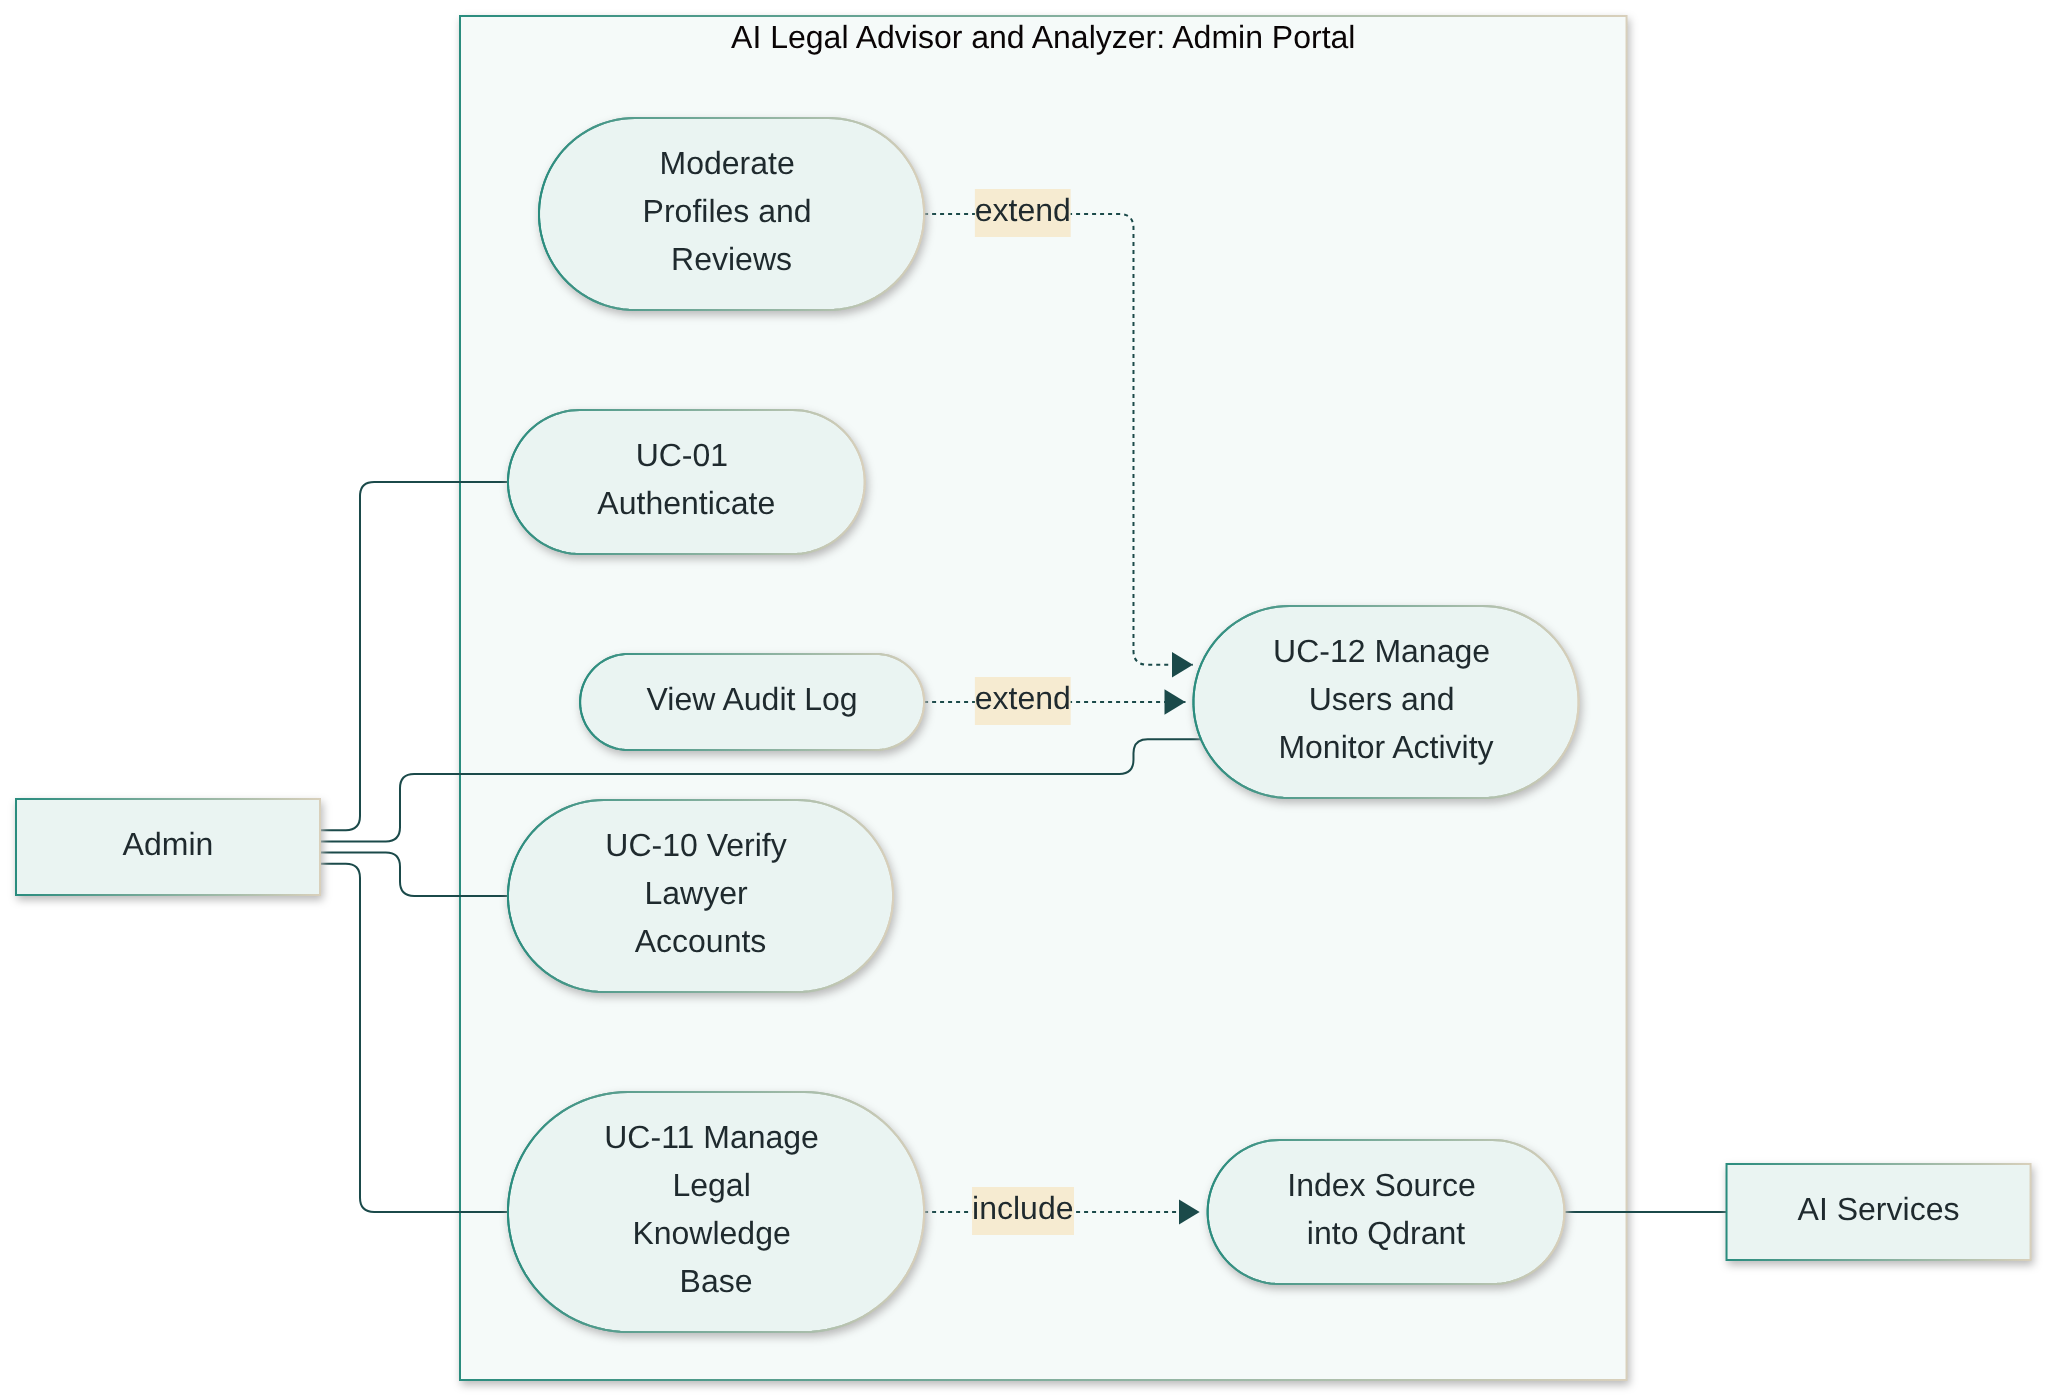
\includegraphics[width=\textwidth,height=0.62\textheight,keepaspectratio]{figures/uc_admin.png}
\caption{Use case diagram, Admin portal}\label{fig:3.3}
\end{figure}

\textbf{Actor interactions.} The User drives the main journey: describe the problem, clarify facts, receive guidance, add evidence, find a lawyer, request a consultation and follow the case. The Lawyer enters the journey only when a User shares a case with consent, and can then respond, communicate and post updates that the User sees on the case timeline. The Admin is not part of individual cases. The Admin keeps the platform trustworthy by verifying lawyers, controlling which legal sources the AI may use, and moderating content.

\needspace{12\baselineskip}
\subsection{Use Case 1: Register and Authenticate}

\begin{center}
\begin{tabular}{|L{2.66cm}|L{12.27cm}|}
\hline\headrow \thd{Field} & \thd{Description} \\ \hline
\textbf{ID} & UC-01 \\ \hline
\textbf{Actors} & User, Lawyer, Admin (primary); Email Service (secondary) \\ \hline
\textbf{Description} & A person creates an account in the chosen role and logs in to the matching portal. \\ \hline
\textbf{Related requirements} & UFR-01 to UFR-04, LFR-01, LFR-02, AFR-01 \\ \hline
\textbf{Preconditions} & The person has a valid email address. For login, the account exists and is not suspended. \\ \hline
\textbf{Postconditions} & A new account is stored with a hashed password and an assigned role (lawyers in \emph{pending verification}); on login, an access token is issued and the role's dashboard is shown. \\ \hline
\end{tabular}
\end{center}

\textbf{Main flow}

\begin{enumerate}
  \item The person opens the registration page and selects a role (User or Lawyer).
  \item The person enters the required details; a lawyer also enters bar enrolment details and uploads the licence.
  \item The system validates the input and checks that the email is not already registered.
  \item The system stores the account with a hashed password and sends a verification email.
  \item The person opens the verification link; the system activates the account.
  \item The person logs in with email and password; the system verifies the credentials, issues an access token and opens the dashboard for the role.
\end{enumerate}

\textbf{Alternative flows}

\begin{itemize}
  \item \emph{3a. Email already registered:} the system shows an error and offers login or password reset.
  \item \emph{5a. Link expired:} the system offers to resend the verification email.
  \item \emph{6a. Wrong credentials:} the system shows a generic error; after repeated failures it temporarily locks login for that account.
  \item \emph{6b. Lawyer not yet verified:} the lawyer can log in and edit the profile, but the profile is not listed in the directory (LFR-04).
  \item \emph{6c. Account suspended:} login is refused with a message to contact support.
\end{itemize}

\needspace{12\baselineskip}
\subsection{Use Case 2: Create Case and Clarify Facts}

\begin{center}
\begin{tabular}{|L{2.99cm}|L{11.94cm}|}
\hline\headrow \thd{Field} & \thd{Description} \\ \hline
\textbf{ID} & UC-02 \\ \hline
\textbf{Actors} & User (primary); AI Services (secondary) \\ \hline
\textbf{Description} & The user describes a legal problem; the system classifies it and asks only the follow-up questions needed to complete the facts. \\ \hline
\textbf{Related requirements} & UFR-06, UFR-07, UFR-08, UFR-16 \\ \hline
\textbf{Preconditions} & The user is logged in. \\ \hline
\textbf{Postconditions} & A case exists with a legal area, topic, problem description and a set of answered follow-up questions; its status is \emph{Clarified}. \\ \hline
\end{tabular}
\end{center}

\textbf{Main flow}

\begin{enumerate}
  \item The user selects ``New case'' and describes the problem in their own words.
  \item The system creates a case and an AI chat session and stores the description.
  \item The system classifies the legal area (property or family) and topic and shows them to the user.
  \item The system compares the stated facts with the facts required for that topic and finds the missing ones.
  \item The system asks one follow-up question; the user answers. Steps 4-5 repeat until no required fact is missing.
  \item The system marks the case as \emph{Clarified} and offers to generate guidance (UC-03).
\end{enumerate}

\textbf{Alternative flows}

\begin{itemize}
  \item \emph{3a. Wrong classification:} the user changes the area or topic and the system recalculates the missing facts.
  \item \emph{3b. Outside property and family law:} the system explains the scope limitation and suggests finding a lawyer (UC-05).
  \item \emph{5a. User does not know the answer:} the user selects ``Not sure''; the fact is recorded as unknown and the guidance will state the assumption.
  \item \emph{5b. User uploads a document instead of answering:} UC-04 runs and extracted facts fill the missing items.
\end{itemize}

\needspace{12\baselineskip}
\subsection{Use Case 3: Obtain AI Legal Guidance}

\begin{center}
\begin{tabular}{|L{2.66cm}|L{12.27cm}|}
\hline\headrow \thd{Field} & \thd{Description} \\ \hline
\textbf{ID} & UC-03 \\ \hline
\textbf{Actors} & User (primary); AI Services (secondary) \\ \hline
\textbf{Description} & The system retrieves relevant Pakistani law and case references and generates plain-language guidance with verified citations. \\ \hline
\textbf{Related requirements} & UFR-09 to UFR-15 \\ \hline
\textbf{Preconditions} & The user is logged in and the case is \emph{Clarified} (UC-02). The knowledge base contains verified, indexed sources. \\ \hline
\textbf{Postconditions} & A guidance record with citations is stored and linked to the case and chat session; the case status becomes \emph{Guidance ready}. \\ \hline
\end{tabular}
\end{center}

\textbf{Main flow}

\begin{enumerate}
  \item The user requests guidance for the case.
  \item The system builds a query from the case facts and creates its embedding with Sentence Transformers.
  \item The system searches Qdrant for the top-k most similar law sections, filtered by legal area.
  \item The system builds a grounded prompt (instructions, retrieved sections, case facts and question) and sends it to the open-source LLM.
  \item The LLM returns a draft answer with source tags.
  \item The system checks that every tag refers to a retrieved section and that every statement has a tag.
  \item The system displays the plain-language answer, the sources list, the evidence checklist and the disclaimer.
\end{enumerate}

\textbf{Alternative flows}

\begin{itemize}
  \item \emph{3a. No section above the relevance threshold:} the system states that no verified source covers the question and recommends a verified lawyer (UFR-13).
  \item \emph{6a. Citation check fails:} the system regenerates once; if it fails again the answer is withheld and the user is told so.
  \item \emph{4a. LLM service unavailable:} the system shows an error, keeps the case, and lets the user retry later (NFR-REL-01).
  \item \emph{7a. Follow-up question:} the user asks a further question and the flow restarts from step 2 within the same session (UFR-15).
\end{itemize}

\needspace{12\baselineskip}
\subsection{Use Case 4: Upload and Analyse Documents}

\begin{center}
\begin{tabular}{|L{3.08cm}|L{11.85cm}|}
\hline\headrow \thd{Field} & \thd{Description} \\ \hline
\textbf{ID} & UC-04 \\ \hline
\textbf{Actors} & User (primary); AI Services (secondary) \\ \hline
\textbf{Description} & The user uploads evidence; the system extracts text, identifies key clauses and updates the evidence checklist. \\ \hline
\textbf{Related requirements} & UFR-17 to UFR-20 \\ \hline
\textbf{Preconditions} & The user is logged in and has an open case. \\ \hline
\textbf{Postconditions} & The document, its extracted text and its clauses are stored; checklist items supported by the document are marked as available. \\ \hline
\end{tabular}
\end{center}

\textbf{Main flow}

\begin{enumerate}
  \item The user selects a case and uploads a PDF, JPG or PNG file.
  \item The system validates type and size and saves the file in the document store.
  \item The system checks whether the PDF has a text layer; if so it extracts text with PyMuPDF, otherwise it runs OCR.
  \item The system identifies key clauses (e.g. parties, rent, term, notice period, dower) and links the document to the case.
  \item The system updates the evidence checklist and shows the extracted clauses to the user.
\end{enumerate}

\textbf{Alternative flows}

\begin{itemize}
  \item \emph{2a. Invalid type or size:} the upload is rejected with a reason.
  \item \emph{3a. OCR text unreadable (low quality):} the system asks for a clearer image; the file is kept but marked \emph{Low quality}.
  \item \emph{4a. No recognised clauses:} the document is stored with its text and the user can label its type manually.
\end{itemize}

\needspace{12\baselineskip}
\subsection{Use Case 5: Search Lawyers and View Public Profile}

\begin{center}
\begin{tabular}{|L{4.04cm}|L{10.89cm}|}
\hline\headrow \thd{Field} & \thd{Description} \\ \hline
\textbf{ID} & UC-05 \\ \hline
\textbf{Actors} & User (primary) \\ \hline
\textbf{Description} & The user finds verified lawyers and reads their public profiles. \\ \hline
\textbf{Related requirements} & UFR-22, UFR-23 \\ \hline
\textbf{Preconditions} & At least one lawyer has been verified (UC-10). Viewing a profile does not require a case. \\ \hline
\textbf{Postconditions} & None (read-only), unless the user continues to UC-06. \\ \hline
\end{tabular}
\end{center}

\textbf{Main flow}

\begin{enumerate}
  \item The user opens the lawyer directory, optionally from a guidance screen that pre-fills the legal area and city.
  \item The user applies filters (specialisation, city, fee range, experience, language, rating).
  \item The system returns verified lawyers that match, sorted by relevance and rating.
  \item The user opens a profile; the system shows headline, about, practice areas, experience, education, bar details, languages, fees, rating and reviews.
\end{enumerate}

\textbf{Alternative flows}

\begin{itemize}
  \item \emph{3a. No match:} the system suggests widening the filters (e.g. nearby cities or a wider fee range).
\end{itemize}

\needspace{12\baselineskip}
\subsection{Use Case 6: Request Consultation and Share Case}

\begin{center}
\begin{tabular}{|L{2.81cm}|L{12.12cm}|}
\hline\headrow \thd{Field} & \thd{Description} \\ \hline
\textbf{ID} & UC-06 \\ \hline
\textbf{Actors} & User (primary); Lawyer (secondary, notified) \\ \hline
\textbf{Description} & The user asks a verified lawyer for a consultation and shares the case after explicit consent. \\ \hline
\textbf{Related requirements} & UFR-21, UFR-24 to UFR-27, UFR-30 \\ \hline
\textbf{Preconditions} & The user is logged in, has a case and has opened a verified lawyer's profile (UC-05). \\ \hline
\textbf{Postconditions} & A consultation with status \emph{Requested} exists; a consent record lists the items shared with the lawyer; the lawyer is notified. \\ \hline
\end{tabular}
\end{center}

\textbf{Main flow}

\begin{enumerate}
  \item The user selects ``Request consultation'' on the lawyer's profile.
  \item The user selects the case, the preferred mode (online or in person), preferred time, and writes a message.
  \item The system shows the consent screen listing what will be shared (case summary, guidance, documents, contact details) and lets the user untick optional items.
  \item The user confirms consent.
  \item The system creates the consultation and consent record, generates the case summary if needed, and notifies the lawyer.
  \item The case timeline shows ``Consultation requested''.
\end{enumerate}

\textbf{Alternative flows}

\begin{itemize}
  \item \emph{4a. User declines consent:} no consultation is created.
  \item \emph{5a. Lawyer has paused new requests:} the system informs the user and suggests other lawyers.
  \item \emph{Later. User revokes sharing:} the lawyer's access ends immediately and the timeline records the revocation (UFR-26).
\end{itemize}

\needspace{12\baselineskip}
\subsection{Use Case 7: Track Case Progress}

\begin{center}
\begin{tabular}{|L{3.96cm}|L{10.97cm}|}
\hline\headrow \thd{Field} & \thd{Description} \\ \hline
\textbf{ID} & UC-07 \\ \hline
\textbf{Actors} & User (primary) \\ \hline
\textbf{Description} & The user follows the case from creation to resolution. \\ \hline
\textbf{Related requirements} & UFR-29, UFR-30, UFR-28 \\ \hline
\textbf{Preconditions} & The user is logged in and owns the case. \\ \hline
\textbf{Postconditions} & The case may be marked \emph{Resolved} or \emph{Closed}; after a completed consultation the user may leave a review. \\ \hline
\end{tabular}
\end{center}

\textbf{Main flow}

\begin{enumerate}
  \item The user opens a case from the dashboard.
  \item The system shows the case status, the timeline of events, the checklist progress and consultation details.
  \item When the lawyer posts an update, the system adds it to the timeline and notifies the user.
  \item When the matter is settled, the user marks the case as \emph{Resolved}.
\end{enumerate}

\textbf{Alternative flows}

\begin{itemize}
  \item \emph{4a. Consultation completed:} the system invites the user to rate and review the lawyer (extension, UFR-28).
  \item \emph{4b. User abandons the case:} the user closes it; the data is kept until the user deletes it.
\end{itemize}

\needspace{12\baselineskip}
\subsection{Use Case 8: Manage Public Profile and Verification Request}

\begin{center}
\begin{tabular}{|L{3.41cm}|L{11.52cm}|}
\hline\headrow \thd{Field} & \thd{Description} \\ \hline
\textbf{ID} & UC-08 \\ \hline
\textbf{Actors} & Lawyer (primary); Admin (secondary) \\ \hline
\textbf{Description} & The lawyer builds a public profile and submits it for verification. \\ \hline
\textbf{Related requirements} & LFR-01, LFR-03 to LFR-05 \\ \hline
\textbf{Preconditions} & The lawyer is registered and logged in. \\ \hline
\textbf{Postconditions} & The profile is saved; a verification request is pending for the Admin. After approval, the profile is listed with a \emph{Verified} badge. \\ \hline
\end{tabular}
\end{center}

\textbf{Main flow}

\begin{enumerate}
  \item The lawyer opens ``My profile'' and edits headline, about, practice areas, experience, education, languages, city, fees and photo.
  \item The system validates and saves the profile, showing a preview of the public page.
  \item The lawyer submits (or re-submits) the verification request with bar details and licence copy.
  \item The system creates a verification request and notifies administrators.
\end{enumerate}

\textbf{Alternative flows}

\begin{itemize}
  \item \emph{4a. Request rejected:} the lawyer sees the reason, corrects the details and re-submits.
  \item \emph{1a. Verified lawyer edits bar details:} the profile returns to \emph{pending verification} for those fields.
\end{itemize}

\needspace{12\baselineskip}
\subsection{Use Case 9: Handle Consultation Requests and Update Case}

\begin{center}
\begin{tabular}{|L{2.85cm}|L{12.08cm}|}
\hline\headrow \thd{Field} & \thd{Description} \\ \hline
\textbf{ID} & UC-09 \\ \hline
\textbf{Actors} & Lawyer (primary); User (secondary, notified) \\ \hline
\textbf{Description} & The lawyer reviews a consultation request, accepts or declines it, and posts progress on the case. \\ \hline
\textbf{Related requirements} & LFR-06 to LFR-11 \\ \hline
\textbf{Preconditions} & The lawyer is verified and logged in; a consultation request with active consent exists. \\ \hline
\textbf{Postconditions} & The consultation status changes (\emph{Accepted}, \emph{Declined}, \emph{Scheduled}, \emph{Completed}); updates appear on the user's case timeline. \\ \hline
\end{tabular}
\end{center}

\textbf{Main flow}

\begin{enumerate}
  \item The lawyer opens the requests list and selects a request.
  \item The system shows the shared case summary, guidance, documents and checklist progress.
  \item The lawyer accepts and confirms a time; the system updates the status to \emph{Scheduled} and notifies the user.
  \item During the matter, the lawyer posts status updates and messages; the system records each on the timeline.
  \item After the consultation, the lawyer marks it \emph{Completed}.
\end{enumerate}

\textbf{Alternative flows}

\begin{itemize}
  \item \emph{3a. Decline:} the lawyer declines with an optional reason; the user is notified and the shared access ends.
  \item \emph{3b. Propose another time:} the lawyer suggests a new time; the user accepts or cancels.
  \item \emph{2a. Consent revoked:} the case is no longer visible and the request is closed.
\end{itemize}

\needspace{12\baselineskip}
\subsection{Use Case 10: Verify Lawyer Accounts}

\begin{center}
\begin{tabular}{|L{3.13cm}|L{11.80cm}|}
\hline\headrow \thd{Field} & \thd{Description} \\ \hline
\textbf{ID} & UC-10 \\ \hline
\textbf{Actors} & Admin (primary); Lawyer (secondary, notified) \\ \hline
\textbf{Description} & The Admin checks a lawyer's submitted credentials and approves or rejects the account. \\ \hline
\textbf{Related requirements} & AFR-02, AFR-09, LFR-04 \\ \hline
\textbf{Preconditions} & The Admin is logged in; a pending verification request exists. \\ \hline
\textbf{Postconditions} & The lawyer's status is \emph{Verified} or \emph{Rejected}; the decision is recorded in the audit log and the lawyer is notified. \\ \hline
\end{tabular}
\end{center}

\textbf{Main flow}

\begin{enumerate}
  \item The Admin opens the verification queue.
  \item The system shows the lawyer's details, bar enrolment information and licence document.
  \item The Admin checks the details against the issuing bar council's records (outside the system) and approves.
  \item The system sets the status to \emph{Verified}, lists the profile in the directory, logs the action and notifies the lawyer.
\end{enumerate}

\textbf{Alternative flows}

\begin{itemize}
  \item \emph{3a. Details do not match:} the Admin rejects with a reason; the lawyer is notified and may re-submit.
  \item \emph{3b. More information needed:} the Admin requests clarification; the request stays pending.
\end{itemize}

\needspace{12\baselineskip}
\subsection{Use Case 11: Manage Legal Knowledge Base}

\begin{center}
\begin{tabular}{|L{2.94cm}|L{11.99cm}|}
\hline\headrow \thd{Field} & \thd{Description} \\ \hline
\textbf{ID} & UC-11 \\ \hline
\textbf{Actors} & Admin (primary); AI Services (secondary) \\ \hline
\textbf{Description} & The Admin adds, verifies, re-indexes or retires a legal source used by the AI assistant. \\ \hline
\textbf{Related requirements} & AFR-05 to AFR-07, NFR-SCL-02 \\ \hline
\textbf{Preconditions} & The Admin is logged in and holds the official text of the source. \\ \hline
\textbf{Postconditions} & The source and its section chunks are stored in MongoDB and their embeddings in Qdrant; only verified, active sources are retrievable. \\ \hline
\end{tabular}
\end{center}

\textbf{Main flow}

\begin{enumerate}
  \item The Admin selects ``Add legal source'' and uploads the official text with metadata (title, type, year, legal area, official URL).
  \item The system extracts the text (PyMuPDF or OCR).
  \item The system splits the text into section-wise chunks and attaches metadata to each.
  \item The system creates an embedding for each chunk and upserts it into Qdrant with the chunk metadata as payload.
  \item The Admin reviews a sample of chunks and marks the source as \emph{Verified}; it becomes retrievable.
\end{enumerate}

\textbf{Alternative flows}

\begin{itemize}
  \item \emph{3a. Section structure not detected:} the system falls back to fixed-length chunks with overlap and flags the source for manual review.
  \item \emph{Later. Source amended:} the Admin uploads the new text; the system re-indexes and retires the old chunks.
  \item \emph{Later. Source repealed:} the Admin retires it; its chunks are excluded from retrieval but kept for past citations.
\end{itemize}

\needspace{12\baselineskip}
\subsection{Use Case 12: Manage Users and Monitor Activity}

\begin{center}
\begin{tabular}{|L{4.31cm}|L{10.62cm}|}
\hline\headrow \thd{Field} & \thd{Description} \\ \hline
\textbf{ID} & UC-12 \\ \hline
\textbf{Actors} & Admin (primary) \\ \hline
\textbf{Description} & The Admin manages accounts, moderates content and monitors platform activity. \\ \hline
\textbf{Related requirements} & AFR-03, AFR-04, AFR-08, AFR-09 \\ \hline
\textbf{Preconditions} & The Admin is logged in. \\ \hline
\textbf{Postconditions} & Account or content changes are applied and recorded in the audit log. \\ \hline
\end{tabular}
\end{center}

\textbf{Main flow}

\begin{enumerate}
  \item The Admin opens the dashboard and views platform statistics.
  \item The Admin searches for a user or lawyer and opens the account.
  \item The Admin suspends, reactivates or removes the account, giving a reason.
  \item The system applies the change, ends active sessions if suspended, and logs the action.
\end{enumerate}

\textbf{Alternative flows}

\begin{itemize}
  \item \emph{2a. Reported content:} the Admin opens the reports queue and removes or keeps the reported profile item or review (extension).
  \item \emph{1a. Audit review:} the Admin filters the audit log by date, administrator or action type (extension).
\end{itemize}

\needspace{12\baselineskip}
\section{System Sequence Diagrams}

The sequence diagrams show how the actors, the Next.js frontend, the FastAPI backend services, the AI services and the data stores interact in the main workflows. Solid arrows are requests and dashed arrows are responses.

\needspace{12\baselineskip}
\subsection{Registration and Login}

% Mermaid source:
% sequenceDiagram
%     autonumber
%     actor P as User / Lawyer
%     participant FE as Next.js Frontend
%     participant API as FastAPI (Auth Service)
%     participant DB as MongoDB
%     participant EM as Email Service
%     P->>FE: Fill registration form (role, details)
%     FE->>API: POST /auth/register
%     API->>DB: Check email exists
%     DB-->>API: Not found
%     API->>API: Hash password (bcrypt/Argon2)
%     API->>DB: Insert account (status = unverified)
%     API->>EM: Send verification link
%     API-->>FE: 201 Created
%     P->>FE: Open verification link
%     FE->>API: GET /auth/verify?token=...
%     API->>DB: Set status = active
%     P->>FE: Enter email and password
%     FE->>API: POST /auth/login
%     API->>DB: Fetch account by email
%     DB-->>API: Account (hash, role, status)
%     alt valid credentials and active
%         API-->>FE: Access token + role
%         FE-->>P: Open role dashboard
%     else invalid or suspended
%         API-->>FE: 401 / 403 error
%         FE-->>P: Show error message
%     end
\begin{figure}[H]\centering
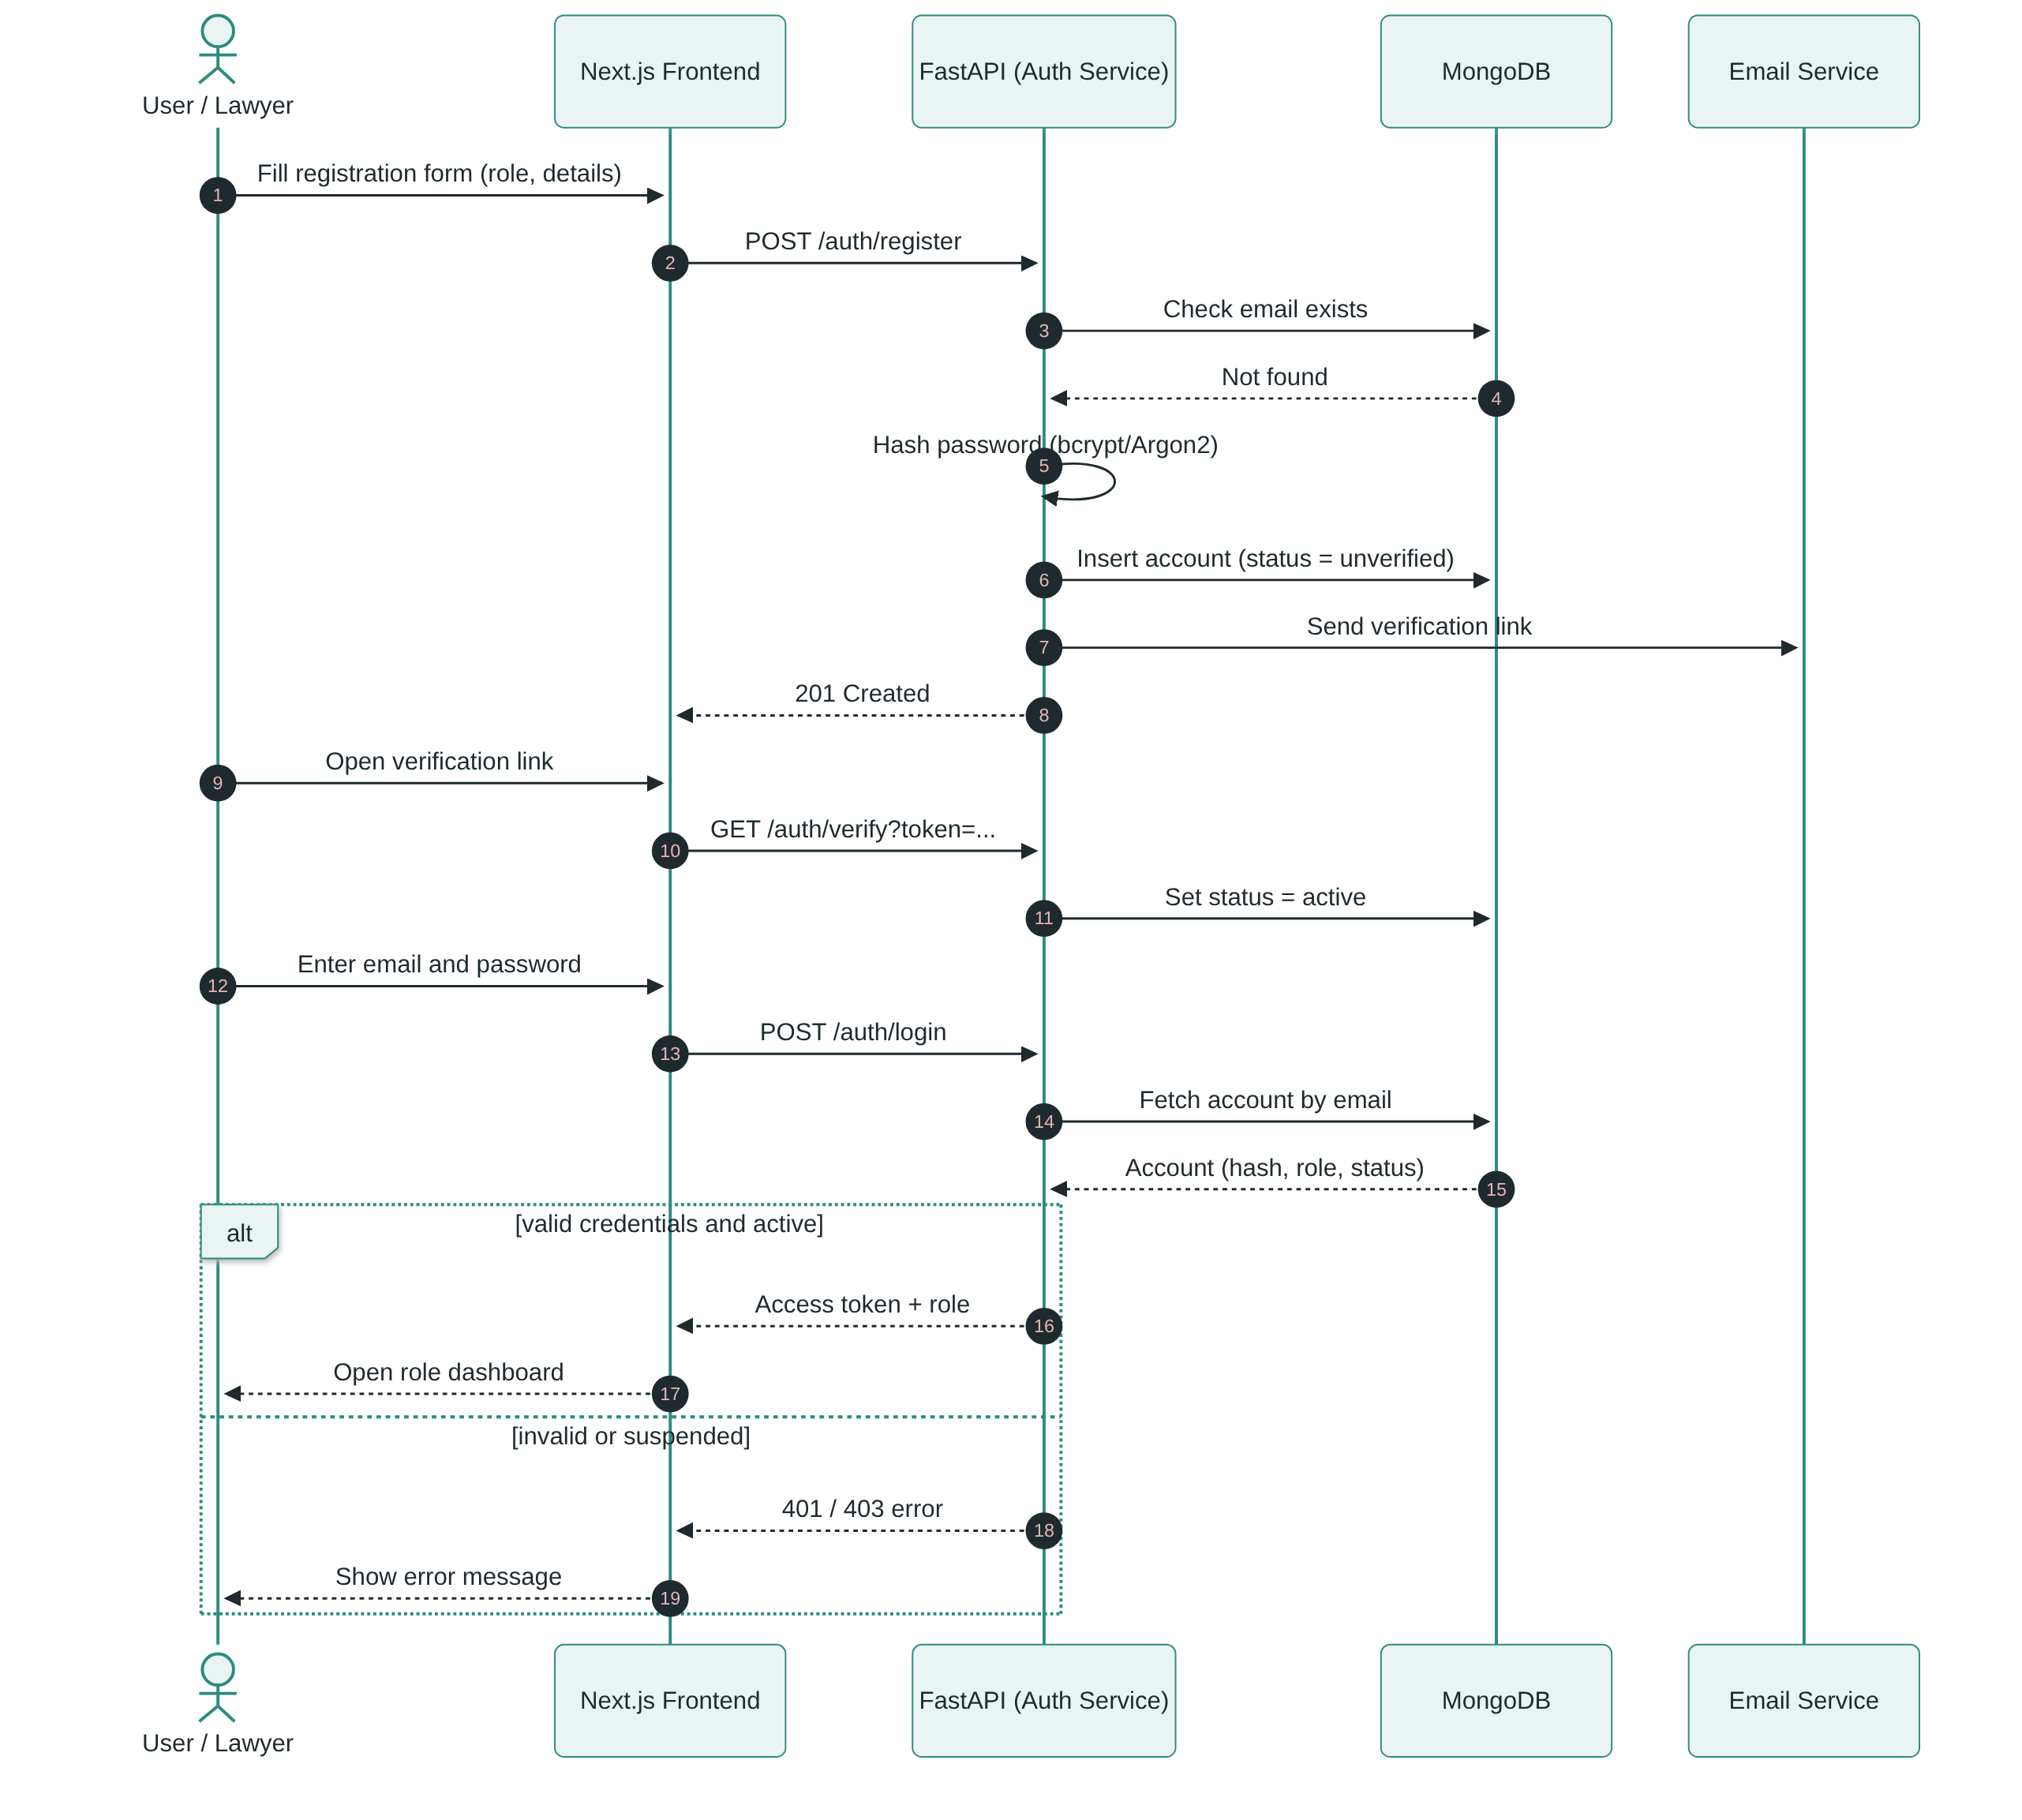
\includegraphics[width=\textwidth,height=0.62\textheight,keepaspectratio]{figures/sd_login.png}
\caption{Sequence diagram, registration and login}\label{fig:3.4}
\end{figure}

The Auth Service never stores plain passwords. It issues a signed token that carries the role, and every later request is checked against that role (NFR-SEC-02). A lawyer account is active after email verification but stays unlisted until UC-10 approves it.

\needspace{12\baselineskip}
\subsection{Case Creation and Fact Clarification}

% Mermaid source:
% sequenceDiagram
%     autonumber
%     actor U as User
%     participant FE as Next.js Frontend
%     participant CS as FastAPI (Case Service)
%     participant FU as Follow-up Engine
%     participant LLM as Open-source LLM
%     participant DB as MongoDB
%     U->>FE: Describe problem
%     FE->>CS: POST /cases (description)
%     CS->>DB: Insert case + chat session
%     CS->>FU: Classify and find missing facts
%     FU->>LLM: Classify area/topic (structured output)
%     LLM-->>FU: Area = property, topic = tenancy
%     FU->>FU: Compare facts with topic checklist
%     FU-->>CS: Missing facts list
%     CS-->>FE: Case created + first follow-up question
%     loop until no required fact is missing
%         FE-->>U: Show question
%         U->>FE: Answer
%         FE->>CS: POST /cases/{id}/answers
%         CS->>DB: Store question and answer
%         CS->>FU: Next missing fact?
%         FU-->>CS: Next question or none
%     end
%     CS->>DB: Update case status = Clarified
%     CS-->>FE: Ready for guidance
\begin{figure}[H]\centering
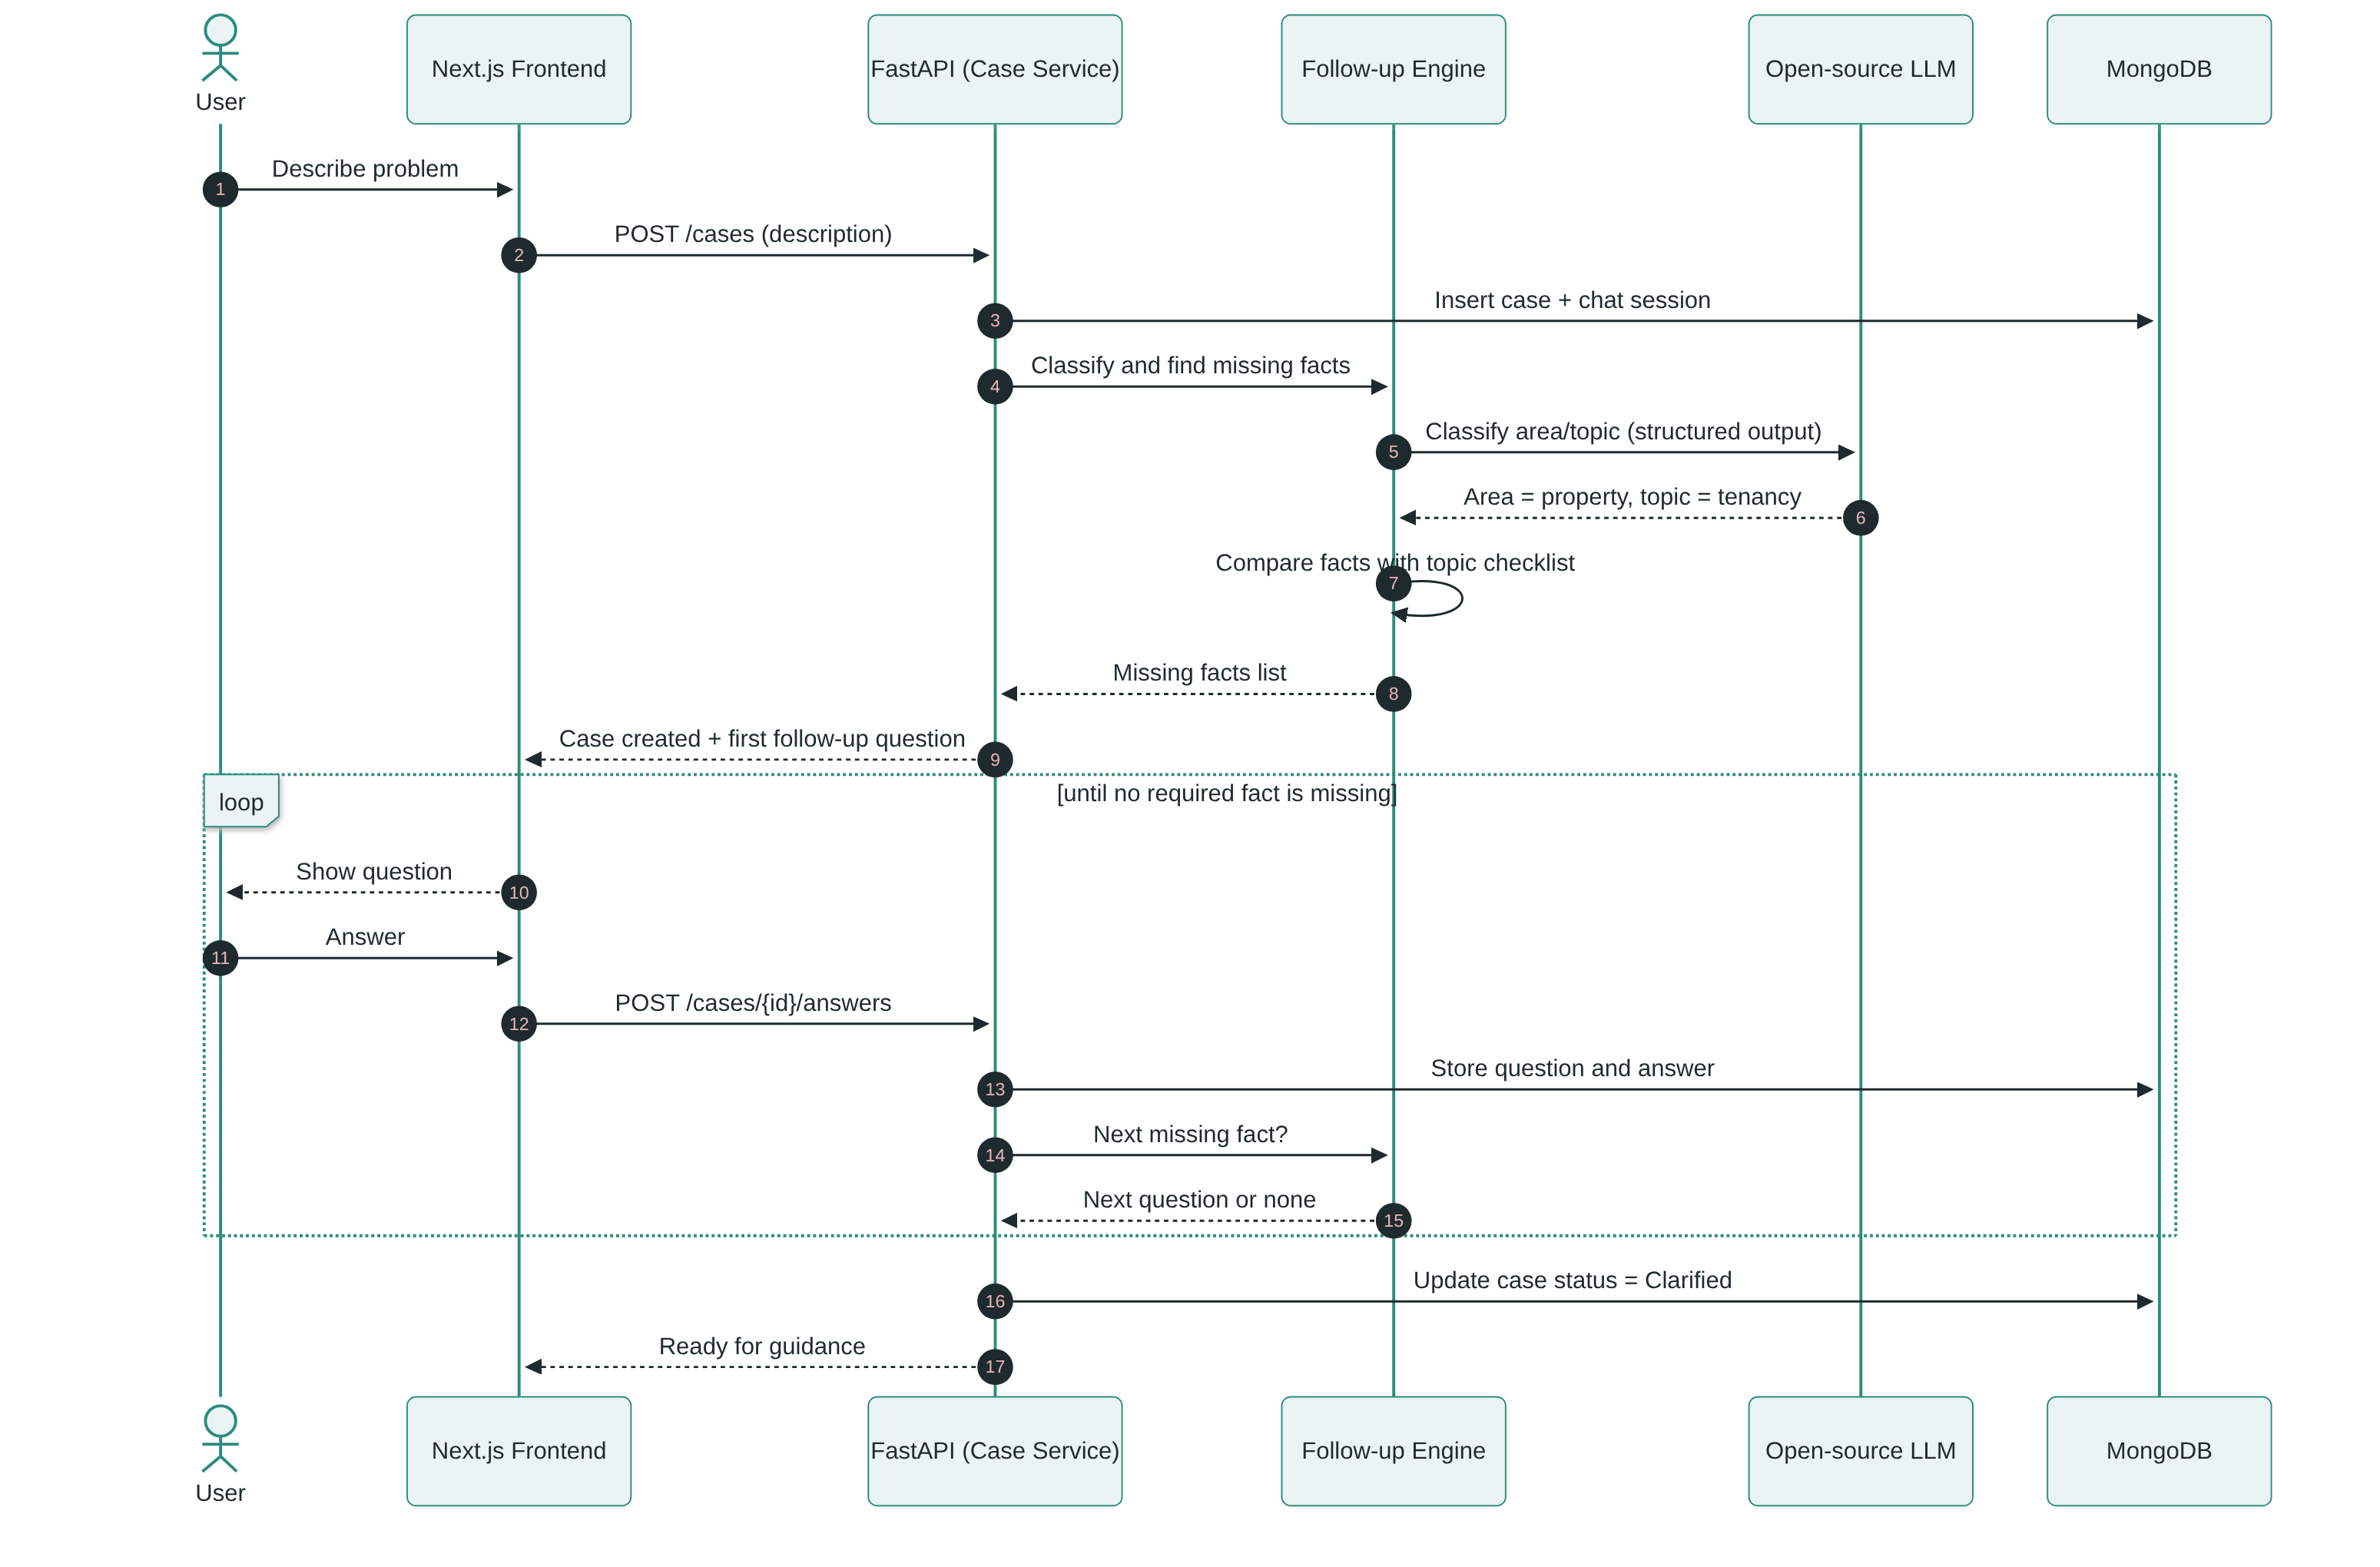
\includegraphics[width=\textwidth,height=0.62\textheight,keepaspectratio]{figures/sd_case.png}
\caption{Sequence diagram, case creation and fact clarification}\label{fig:3.5}
\end{figure}

The LLM classifies the problem, but the list of required facts per topic is defined by the team and stored with the system. As a result, the follow-up questions are predictable and can be tested.

\needspace{12\baselineskip}
\subsection{AI Legal Guidance (RAG)}

% Mermaid source:
% sequenceDiagram
%     autonumber
%     actor U as User
%     participant FE as Next.js Frontend
%     participant RAG as FastAPI (RAG Service)
%     participant EMB as Sentence Transformers
%     participant QD as Qdrant
%     participant LLM as Open-source LLM
%     participant CC as Citation Checker
%     participant DB as MongoDB
%     U->>FE: Request guidance
%     FE->>RAG: POST /cases/{id}/guidance
%     RAG->>DB: Load case facts and history
%     RAG->>EMB: Embed query
%     EMB-->>RAG: Query vector
%     RAG->>QD: Similarity search (top-k, filter: legal area)
%     QD-->>RAG: Sections + payload (source, section, score)
%     alt no section above threshold
%         RAG-->>FE: "No verified source found" + lawyer suggestion
%     else relevant sections found
%         RAG->>LLM: Grounded prompt (rules + sections + facts)
%         LLM-->>RAG: Draft answer with [S1], [S2] tags
%         RAG->>CC: Verify tags against retrieved sections
%         alt citations valid
%             CC-->>RAG: Pass
%             RAG->>DB: Save guidance + citations + checklist
%             RAG-->>FE: Answer, sources, checklist, disclaimer
%         else citation check fails
%             CC-->>RAG: Fail
%             RAG->>LLM: Regenerate once
%             RAG-->>FE: Answer if it passes, otherwise withheld
%         end
%     end
%     FE-->>U: Display result
\begin{figure}[H]\centering
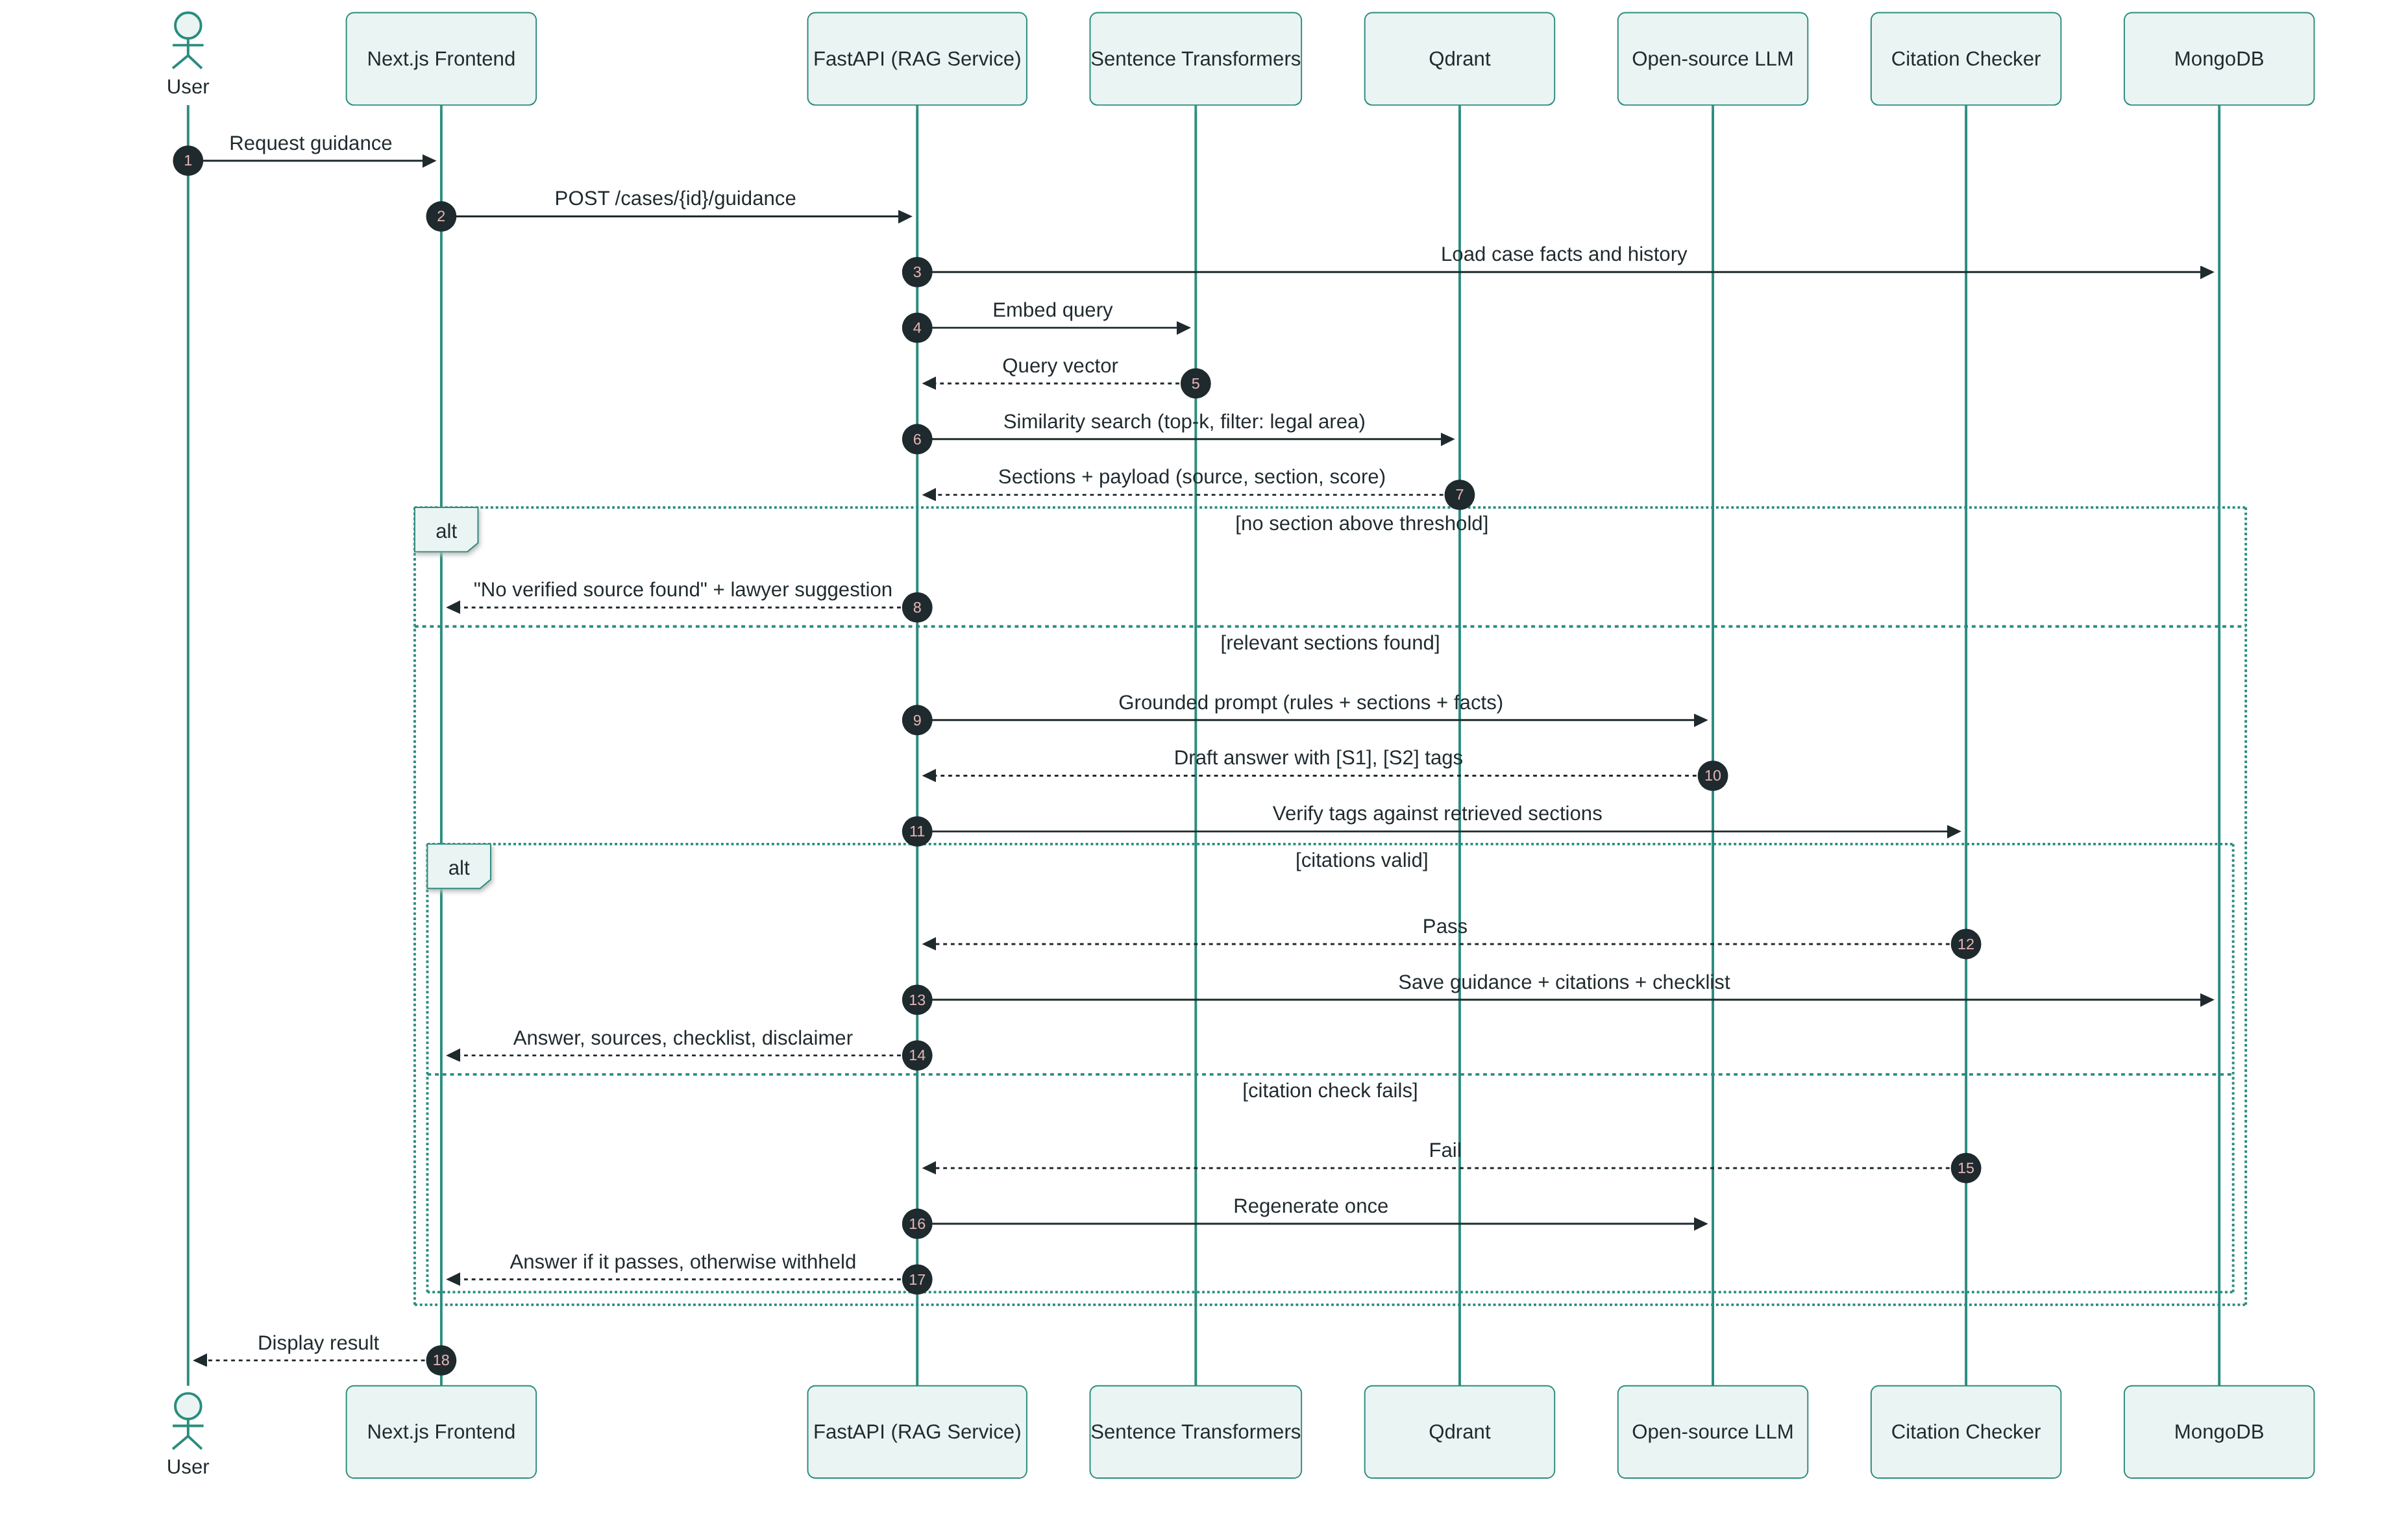
\includegraphics[width=\textwidth,height=0.62\textheight,keepaspectratio]{figures/sd_rag.png}
\caption{Sequence diagram, AI legal guidance with retrieval and citation verification}\label{fig:3.6}
\end{figure}

This is the central workflow of the project. The LLM never queries the databases. The RAG Service retrieves the sections first and passes only those sections to the LLM, then checks the returned citations before anything is displayed. This design responds directly to the hallucination findings in \cite{r8} and \cite{r9}.

\needspace{12\baselineskip}
\subsection{Document Upload, OCR and Evidence Checklist}

% Mermaid source:
% sequenceDiagram
%     autonumber
%     actor U as User
%     participant FE as Next.js Frontend
%     participant DP as FastAPI (Document Processor)
%     participant FS as File Store
%     participant PDF as PyMuPDF
%     participant OCR as OCR Engine
%     participant LLM as Open-source LLM
%     participant DB as MongoDB
%     U->>FE: Upload file to case
%     FE->>DP: POST /cases/{id}/documents
%     DP->>DP: Validate type and size
%     DP->>FS: Save file
%     DP->>DB: Insert document (status = processing)
%     DP-->>FE: 202 Accepted
%     alt PDF with text layer
%         DP->>PDF: Extract text
%         PDF-->>DP: Text
%     else scan or image
%         DP->>OCR: Recognise text
%         OCR-->>DP: Text
%     end
%     DP->>LLM: Extract key clauses (structured fields)
%     LLM-->>DP: Clauses (parties, rent, term, notice...)
%     DP->>DB: Save text and clauses, update checklist items
%     DP-->>FE: Notify processing complete
%     FE-->>U: Show clauses and updated checklist
\begin{figure}[H]\centering
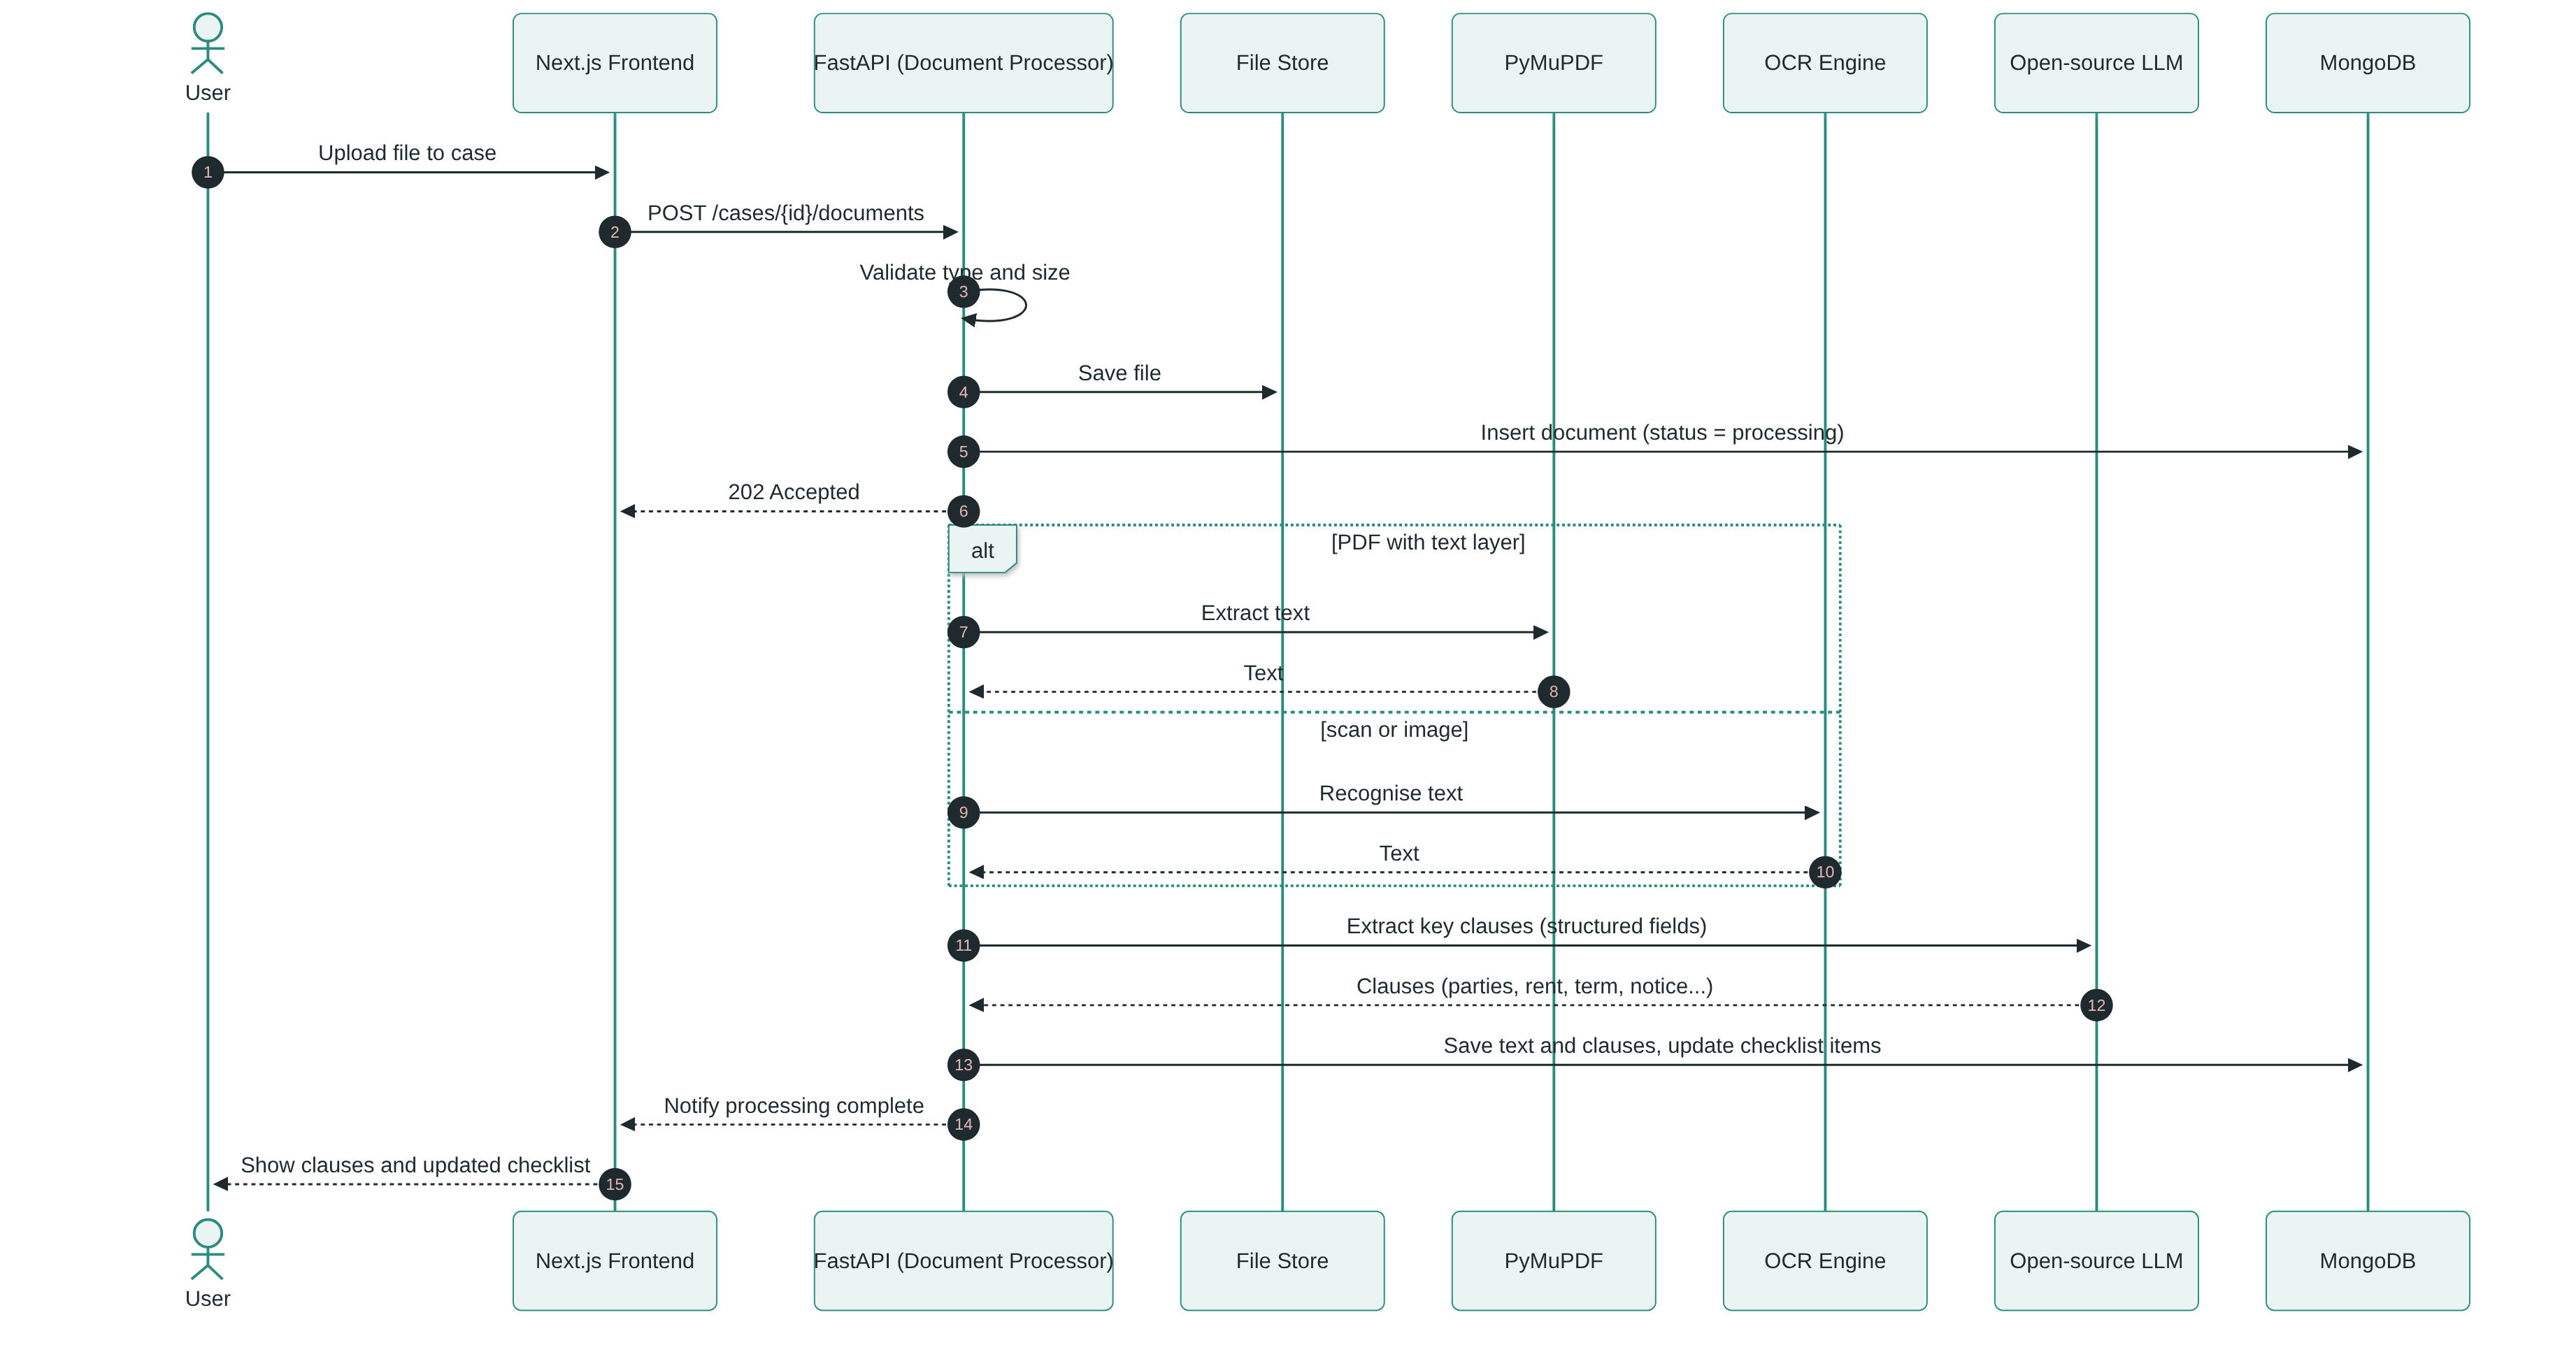
\includegraphics[width=\textwidth,height=0.62\textheight,keepaspectratio]{figures/sd_docs.png}
\caption{Sequence diagram, document upload and analysis}\label{fig:3.7}
\end{figure}

Extraction runs asynchronously, so the user is never blocked while a large scan is processed (NFR-REL-02). Clause extraction uses the user's own document as input. It does not depend on legal retrieval and produces structured fields that the user can see and correct.

\needspace{12\baselineskip}
\subsection{Lawyer Search, Public Profile and Consultation Request}

% Mermaid source:
% sequenceDiagram
%     autonumber
%     actor U as User
%     participant FE as Next.js Frontend
%     participant LD as FastAPI (Lawyer Directory)
%     participant CN as FastAPI (Consultation Service)
%     participant DB as MongoDB
%     actor L as Lawyer
%     U->>FE: Search with filters
%     FE->>LD: GET /lawyers?area=&city=&fee=&lang=&rating=
%     LD->>DB: Query verified lawyers
%     DB-->>LD: Matching profiles
%     LD-->>FE: Results
%     U->>FE: Open public profile
%     FE->>LD: GET /lawyers/{id}
%     LD-->>FE: Profile, experience, education, reviews
%     U->>FE: Request consultation (case, mode, time, message)
%     FE-->>U: Consent screen (items to share)
%     U->>FE: Confirm consent
%     FE->>CN: POST /consultations
%     CN->>DB: Insert consultation (Requested) + consent record
%     CN->>DB: Add timeline event to case
%     CN-->>FE: Request sent
%     CN--)L: Notification: new consultation request
\begin{figure}[H]\centering
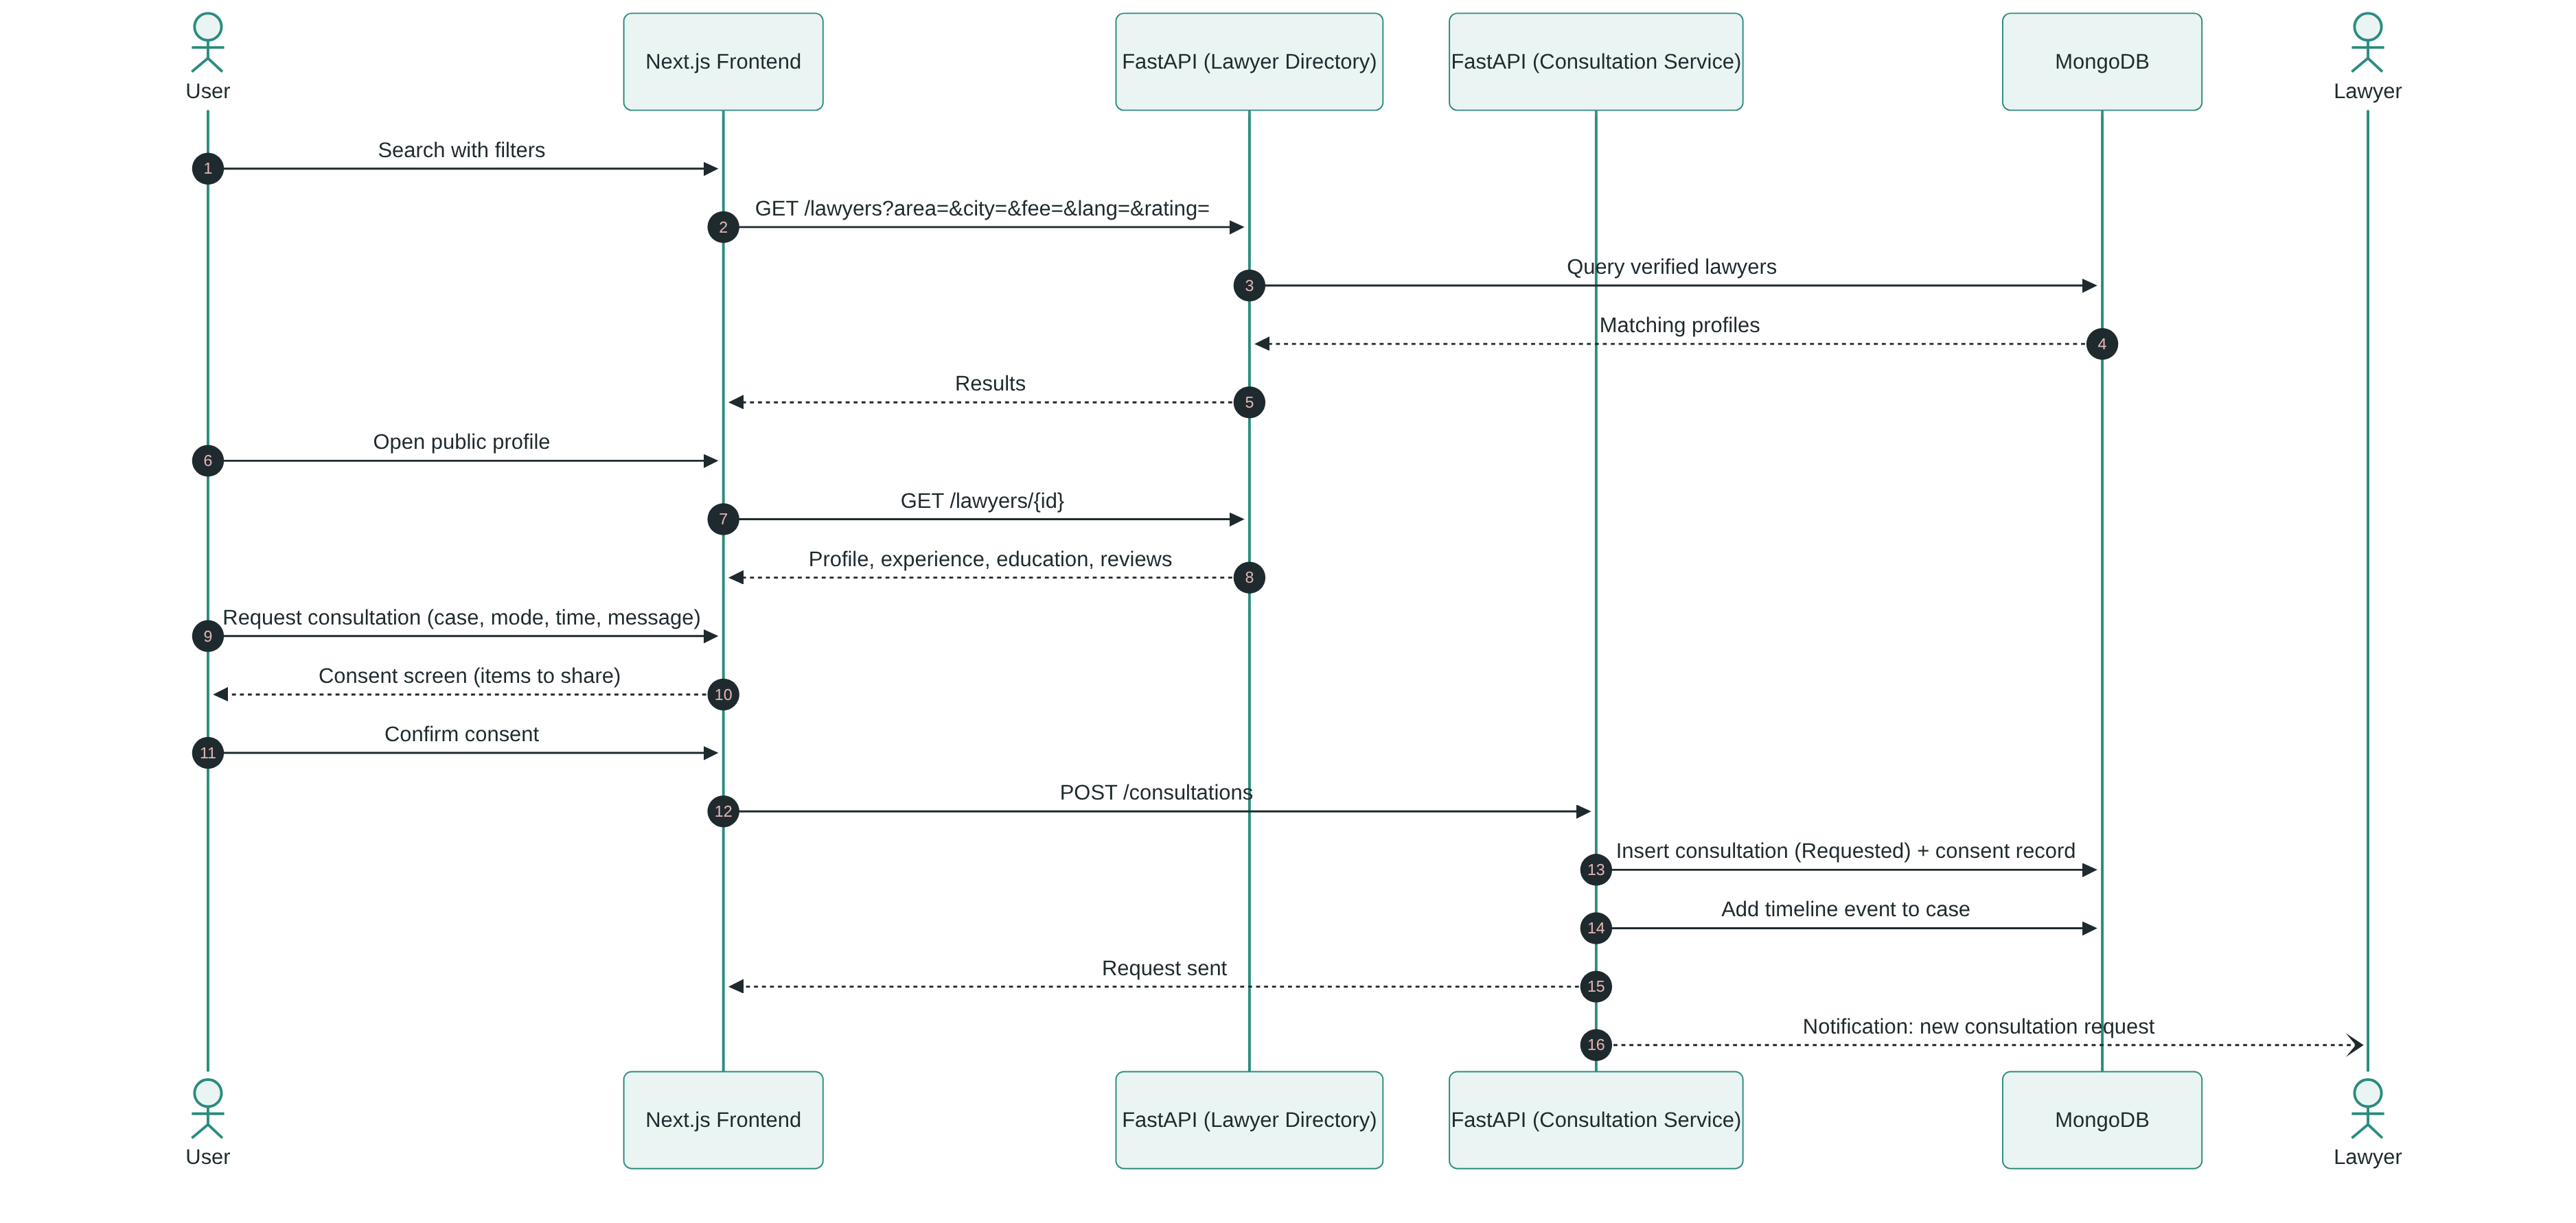
\includegraphics[width=\textwidth,height=0.62\textheight,keepaspectratio]{figures/sd_consult.png}
\caption{Sequence diagram, lawyer search and consultation request}\label{fig:3.8}
\end{figure}

Only lawyers with \emph{Verified} status are returned. Contact details are released only after the lawyer accepts (NFR-PRV-02). The consent record defines exactly which case items the lawyer may read.

\needspace{12\baselineskip}
\subsection{Lawyer Handles Consultation and Updates Case}

% Mermaid source:
% sequenceDiagram
%     autonumber
%     actor L as Lawyer
%     participant FE as Next.js (Lawyer Portal)
%     participant CN as FastAPI (Consultation Service)
%     participant CS as FastAPI (Case Service)
%     participant DB as MongoDB
%     actor U as User
%     L->>FE: Open request
%     FE->>CN: GET /consultations/{id}
%     CN->>DB: Check consent active
%     DB-->>CN: Consent + shared items
%     CN-->>FE: Case summary, guidance, documents
%     L->>FE: Accept and confirm time
%     FE->>CN: PATCH /consultations/{id} (Scheduled)
%     CN->>DB: Update status
%     CN--)U: Notification: consultation scheduled
%     L->>FE: Post status update and note
%     FE->>CS: POST /cases/{id}/updates
%     CS->>DB: Insert status update (timeline)
%     CS--)U: Notification: case updated
%     L->>FE: Mark consultation completed
%     FE->>CN: PATCH /consultations/{id} (Completed)
%     CN--)U: Invitation to review lawyer
\begin{figure}[H]\centering
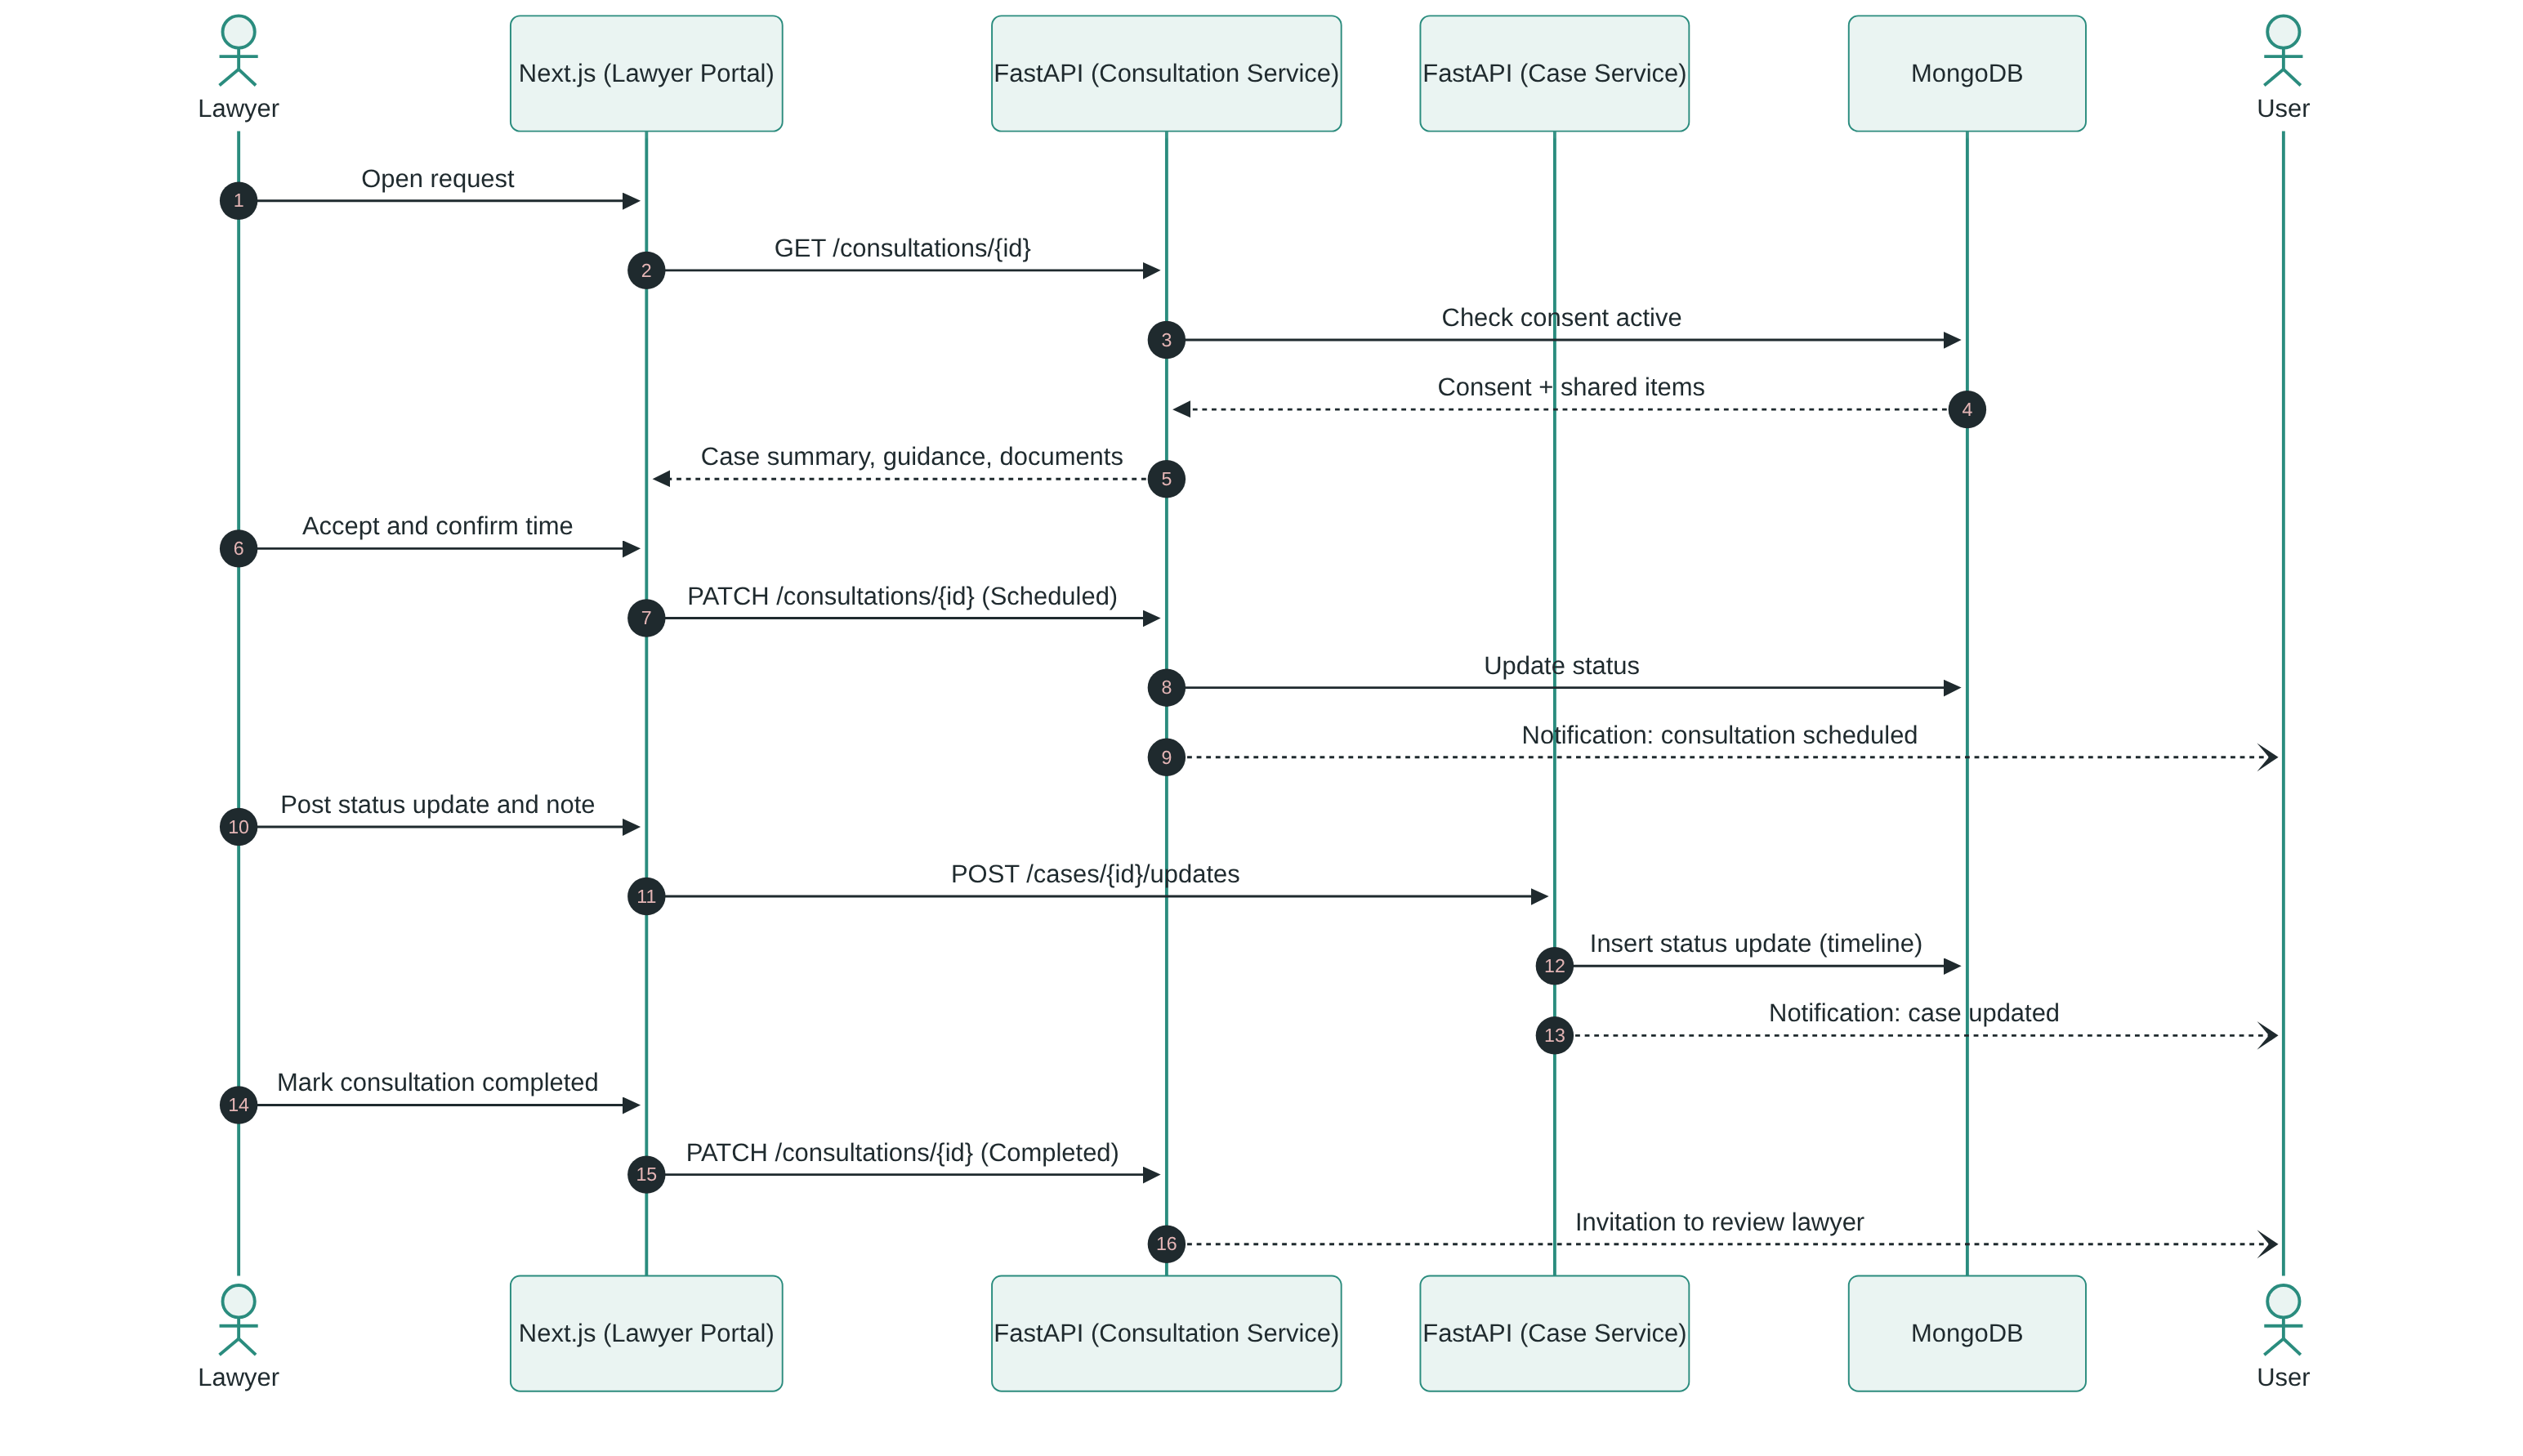
\includegraphics[width=\textwidth,height=0.62\textheight,keepaspectratio]{figures/sd_lawyer.png}
\caption{Sequence diagram, lawyer response and case update}\label{fig:3.9}
\end{figure}

Every read by the lawyer is checked against the active consent record. If the user revokes consent, the next request is refused and the consultation is closed.

\needspace{12\baselineskip}
\subsection{Admin Verifies a Lawyer}

% Mermaid source:
% sequenceDiagram
%     autonumber
%     actor A as Admin
%     participant FE as Next.js (Admin Portal)
%     participant AS as FastAPI (Admin Service)
%     participant DB as MongoDB
%     participant FS as File Store
%     actor L as Lawyer
%     A->>FE: Open verification queue
%     FE->>AS: GET /admin/verifications?status=pending
%     AS->>DB: Fetch pending requests
%     DB-->>AS: Requests
%     AS-->>FE: List
%     A->>FE: Open request
%     FE->>AS: GET /admin/verifications/{id}
%     AS->>FS: Fetch licence document
%     AS-->>FE: Details + document
%     alt approve
%         A->>FE: Approve
%         FE->>AS: POST /admin/verifications/{id}/approve
%         AS->>DB: Lawyer status = Verified, list profile
%     else reject
%         A->>FE: Reject with reason
%         FE->>AS: POST /admin/verifications/{id}/reject
%         AS->>DB: Lawyer status = Rejected
%     end
%     AS->>DB: Write audit log entry
%     AS--)L: Notification of decision
\begin{figure}[H]\centering
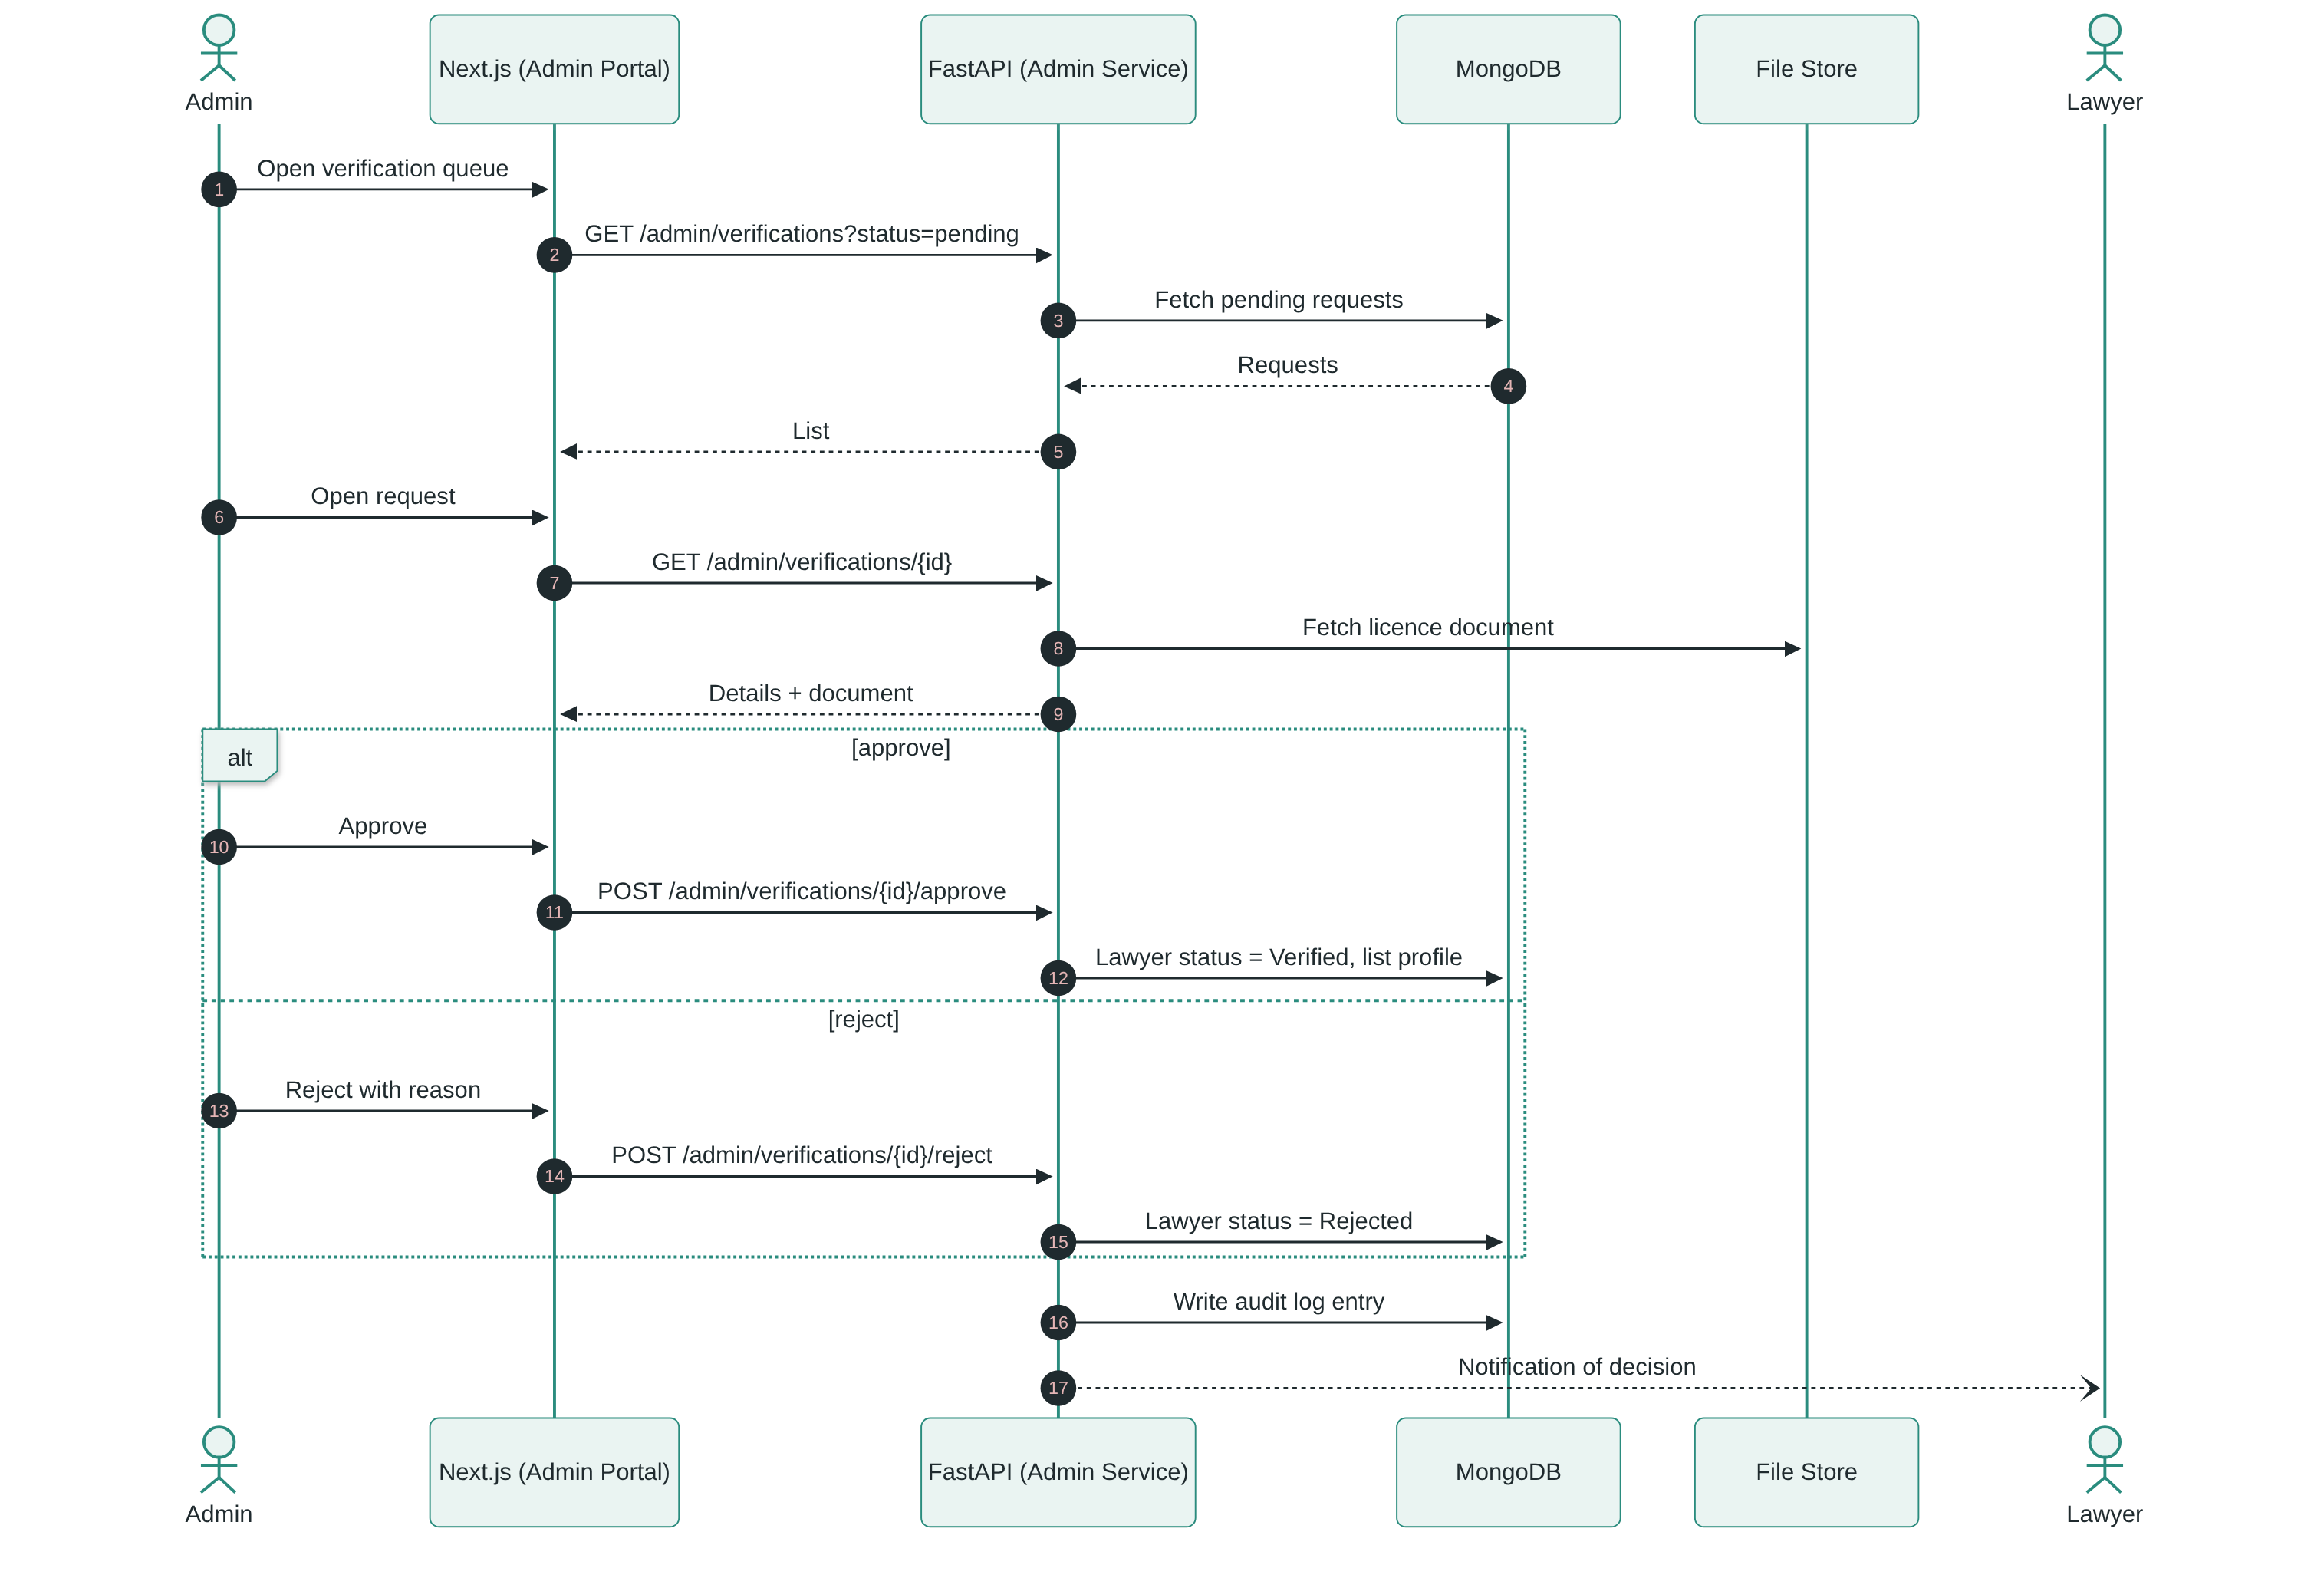
\includegraphics[width=\textwidth,height=0.62\textheight,keepaspectratio]{figures/sd_verify.png}
\caption{Sequence diagram, lawyer verification}\label{fig:3.10}
\end{figure}

\needspace{12\baselineskip}
\subsection{Admin Adds a Legal Source (Knowledge Base Ingestion)}

% Mermaid source:
% sequenceDiagram
%     autonumber
%     actor A as Admin
%     participant FE as Next.js (Admin Portal)
%     participant KB as FastAPI (Knowledge Base Builder)
%     participant PDF as PyMuPDF / OCR
%     participant EMB as Sentence Transformers
%     participant QD as Qdrant
%     participant DB as MongoDB
%     A->>FE: Upload official text + metadata
%     FE->>KB: POST /admin/sources
%     KB->>DB: Insert source (status = processing)
%     KB->>PDF: Extract text
%     PDF-->>KB: Text
%     KB->>KB: Split into section-wise chunks + metadata
%     loop for each chunk
%         KB->>EMB: Embed chunk text
%         EMB-->>KB: Vector
%         KB->>QD: Upsert point (vector, payload: chunk id, area, topic)
%         KB->>DB: Insert chunk record
%     end
%     KB->>DB: Source status = awaiting review
%     KB-->>FE: Ingestion complete
%     A->>FE: Review sample chunks and mark verified
%     FE->>KB: PATCH /admin/sources/{id} (Verified)
%     KB->>DB: Source active and retrievable
\begin{figure}[H]\centering
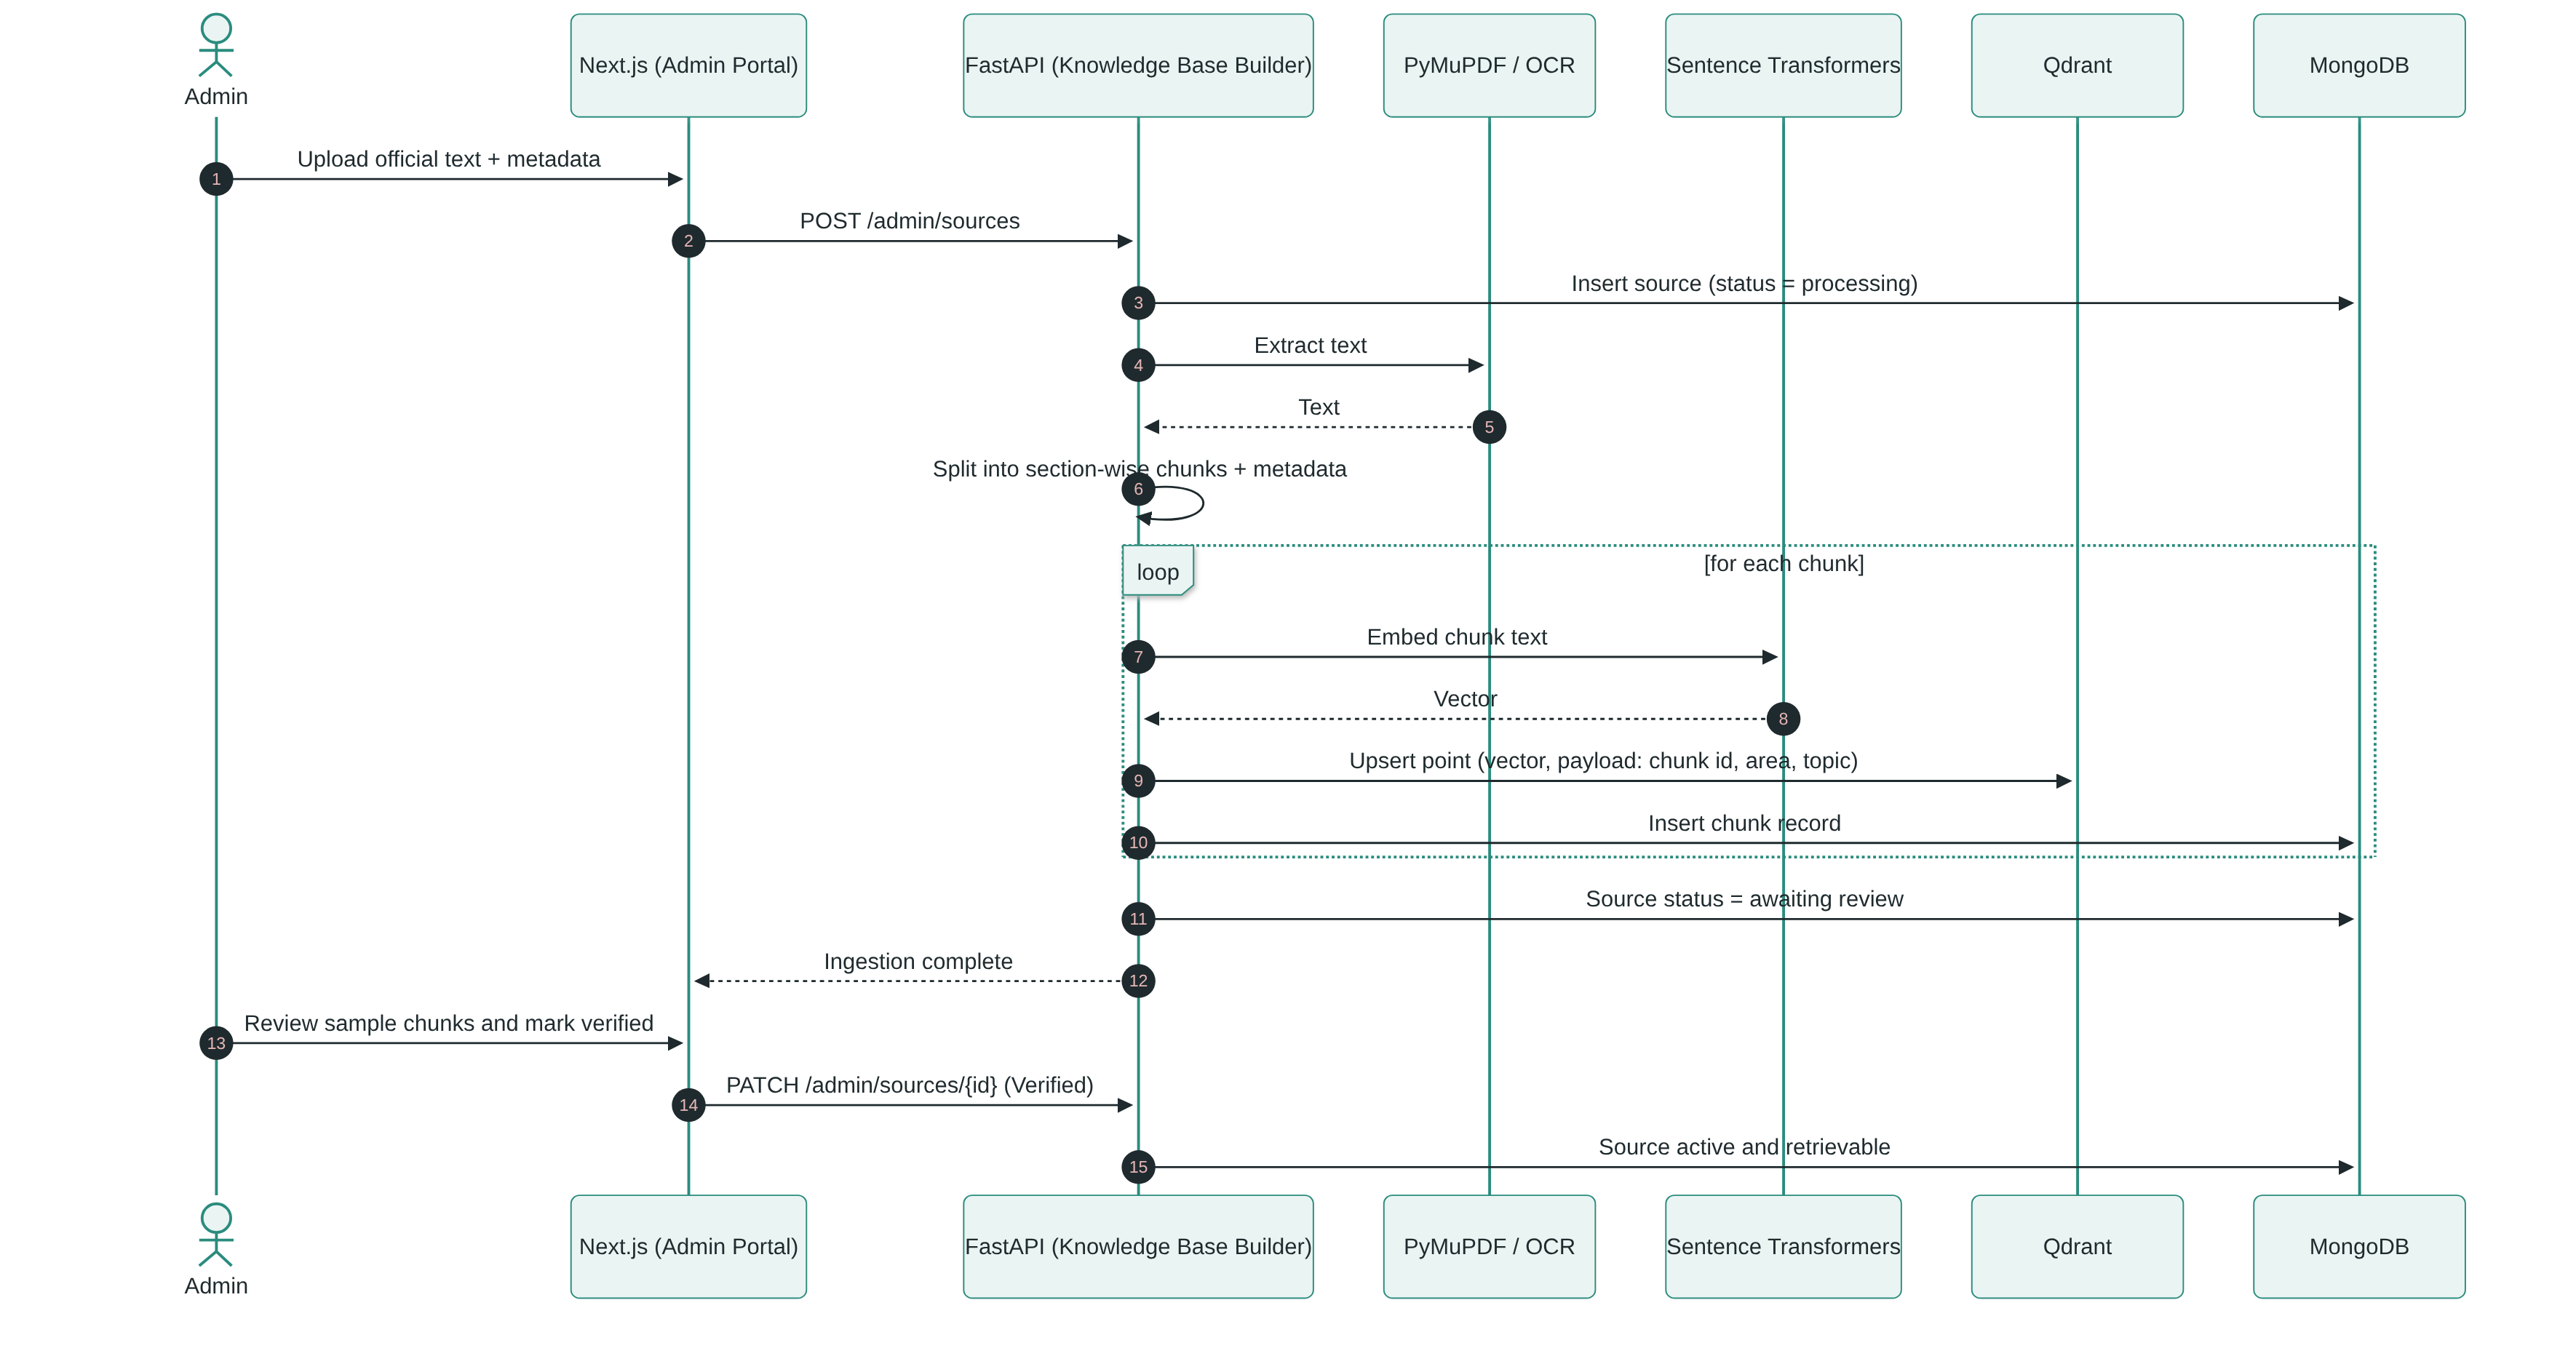
\includegraphics[width=\textwidth,height=0.62\textheight,keepaspectratio]{figures/sd_ingest.png}
\caption{Sequence diagram, legal source ingestion}\label{fig:3.11}
\end{figure}

This is the offline phase of the RAG pipeline described in Chapter 1. Each Qdrant point carries the chunk identifier in its payload, so any retrieved vector can be traced back to its source and section for citation.

\needspace{12\baselineskip}
\section{Domain Model}

The domain model identifies the main entities of the system, their key attributes, and their relationships with cardinalities. \texttt{Account} is an abstract generalisation of the three actor types: \texttt{User} (citizen), \texttt{Lawyer} and \texttt{Admin}. \texttt{Case} is the central entity of the model.

% Mermaid source:
% classDiagram
%     direction LR
%     class Account {
%         <<abstract>>
%         +accountId
%         +fullName
%         +email
%         +phone
%         +passwordHash
%         +role
%         +status
%         +createdAt
%     }
%     class User {
%         +city
%         +preferredLanguage
%     }
%     class Lawyer {
%         +headline
%         +about
%         +practiceAreas
%         +barEnrolmentNo
%         +barCouncil
%         +city
%         +officeAddress
%         +languages
%         +feeMin
%         +feeMax
%         +experienceYears
%         +verificationStatus
%         +ratingAverage
%         +acceptingRequests
%     }
%     class Admin {
%         +adminLevel
%     }
%     class Experience {
%         +title
%         +organisation
%         +startDate
%         +endDate
%         +description
%     }
%     class Qualification {
%         +degree
%         +institution
%         +year
%     }
%     class VerificationRequest {
%         +licenceDocument
%         +submittedAt
%         +decision
%         +reason
%         +decidedAt
%     }
%     class Case {
%         +caseId
%         +title
%         +legalArea
%         +topic
%         +description
%         +status
%         +createdAt
%         +updatedAt
%     }
%     class FollowUpQuestion {
%         +requiredFact
%         +question
%         +answer
%         +answeredAt
%     }
%     class ChatSession {
%         +sessionId
%         +startedAt
%     }
%     class ChatMessage {
%         +sender
%         +text
%         +sentAt
%     }
%     class LegalGuidance {
%         +answerText
%         +modelName
%         +citationCheckPassed
%         +generatedAt
%     }
%     class Citation {
%         +label
%         +quotedText
%         +similarityScore
%     }
%     class LegalSource {
%         +title
%         +sourceType
%         +year
%         +legalArea
%         +officialUrl
%         +status
%     }
%     class LegalSection {
%         +sectionRef
%         +heading
%         +text
%         +topic
%         +vectorId
%     }
%     class LegalDocument {
%         +fileName
%         +fileType
%         +storagePath
%         +extractionMethod
%         +extractedText
%         +uploadedAt
%     }
%     class Clause {
%         +clauseType
%         +value
%     }
%     class EvidenceChecklist {
%         +createdAt
%     }
%     class ChecklistItem {
%         +description
%         +required
%         +available
%     }
%     class Consultation {
%         +mode
%         +requestedTime
%         +scheduledTime
%         +status
%         +message
%     }
%     class ConsentRecord {
%         +sharedItems
%         +grantedAt
%         +revokedAt
%     }
%     class ConsultationMessage {
%         +senderRole
%         +text
%         +sentAt
%     }
%     class CaseStatusUpdate {
%         +status
%         +note
%         +postedBy
%         +postedAt
%     }
%     class Review {
%         +rating
%         +comment
%         +createdAt
%     }
%     class Notification {
%         +type
%         +text
%         +read
%         +createdAt
%     }
%     class AuditLog {
%         +action
%         +targetType
%         +targetId
%         +reason
%         +timestamp
%     }
% 
%     Account <|-- User
%     Account <|-- Lawyer
%     Account <|-- Admin
%     Lawyer "1" *-- "0..*" Experience : lists
%     Lawyer "1" *-- "0..*" Qualification : holds
%     Lawyer "1" -- "1..*" VerificationRequest : submits
%     Admin "1" -- "0..*" VerificationRequest : decides
%     User "1" -- "0..*" Case : opens
%     Case "1" *-- "0..*" FollowUpQuestion : clarified by
%     Case "1" *-- "1..*" ChatSession : discussed in
%     ChatSession "1" *-- "1..*" ChatMessage : contains
%     ChatMessage "1" -- "0..1" LegalGuidance : delivers
%     LegalGuidance "1" *-- "1..*" Citation : supported by
%     Citation "0..*" --> "1" LegalSection : quotes
%     LegalSource "1" *-- "1..*" LegalSection : divided into
%     Admin "1" -- "0..*" LegalSource : verifies
%     Case "1" *-- "0..*" LegalDocument : has
%     LegalDocument "1" *-- "0..*" Clause : contains
%     Case "1" *-- "0..1" EvidenceChecklist : needs
%     EvidenceChecklist "1" *-- "1..*" ChecklistItem : lists
%     ChecklistItem "0..*" --> "0..1" LegalDocument : satisfied by
%     Case "1" -- "0..*" Consultation : discussed in
%     User "1" -- "0..*" Consultation : requests
%     Lawyer "1" -- "0..*" Consultation : handles
%     Consultation "1" *-- "1" ConsentRecord : governed by
%     Consultation "1" *-- "0..*" ConsultationMessage : contains
%     Case "1" *-- "0..*" CaseStatusUpdate : history
%     Consultation "1" -- "0..1" Review : rated by
%     User "1" -- "0..*" Review : writes
%     Lawyer "1" -- "0..*" Review : receives
%     Account "1" -- "0..*" Notification : receives
%     Admin "1" -- "0..*" AuditLog : recorded in
\begin{landscape}
\begin{figure}[p]\centering
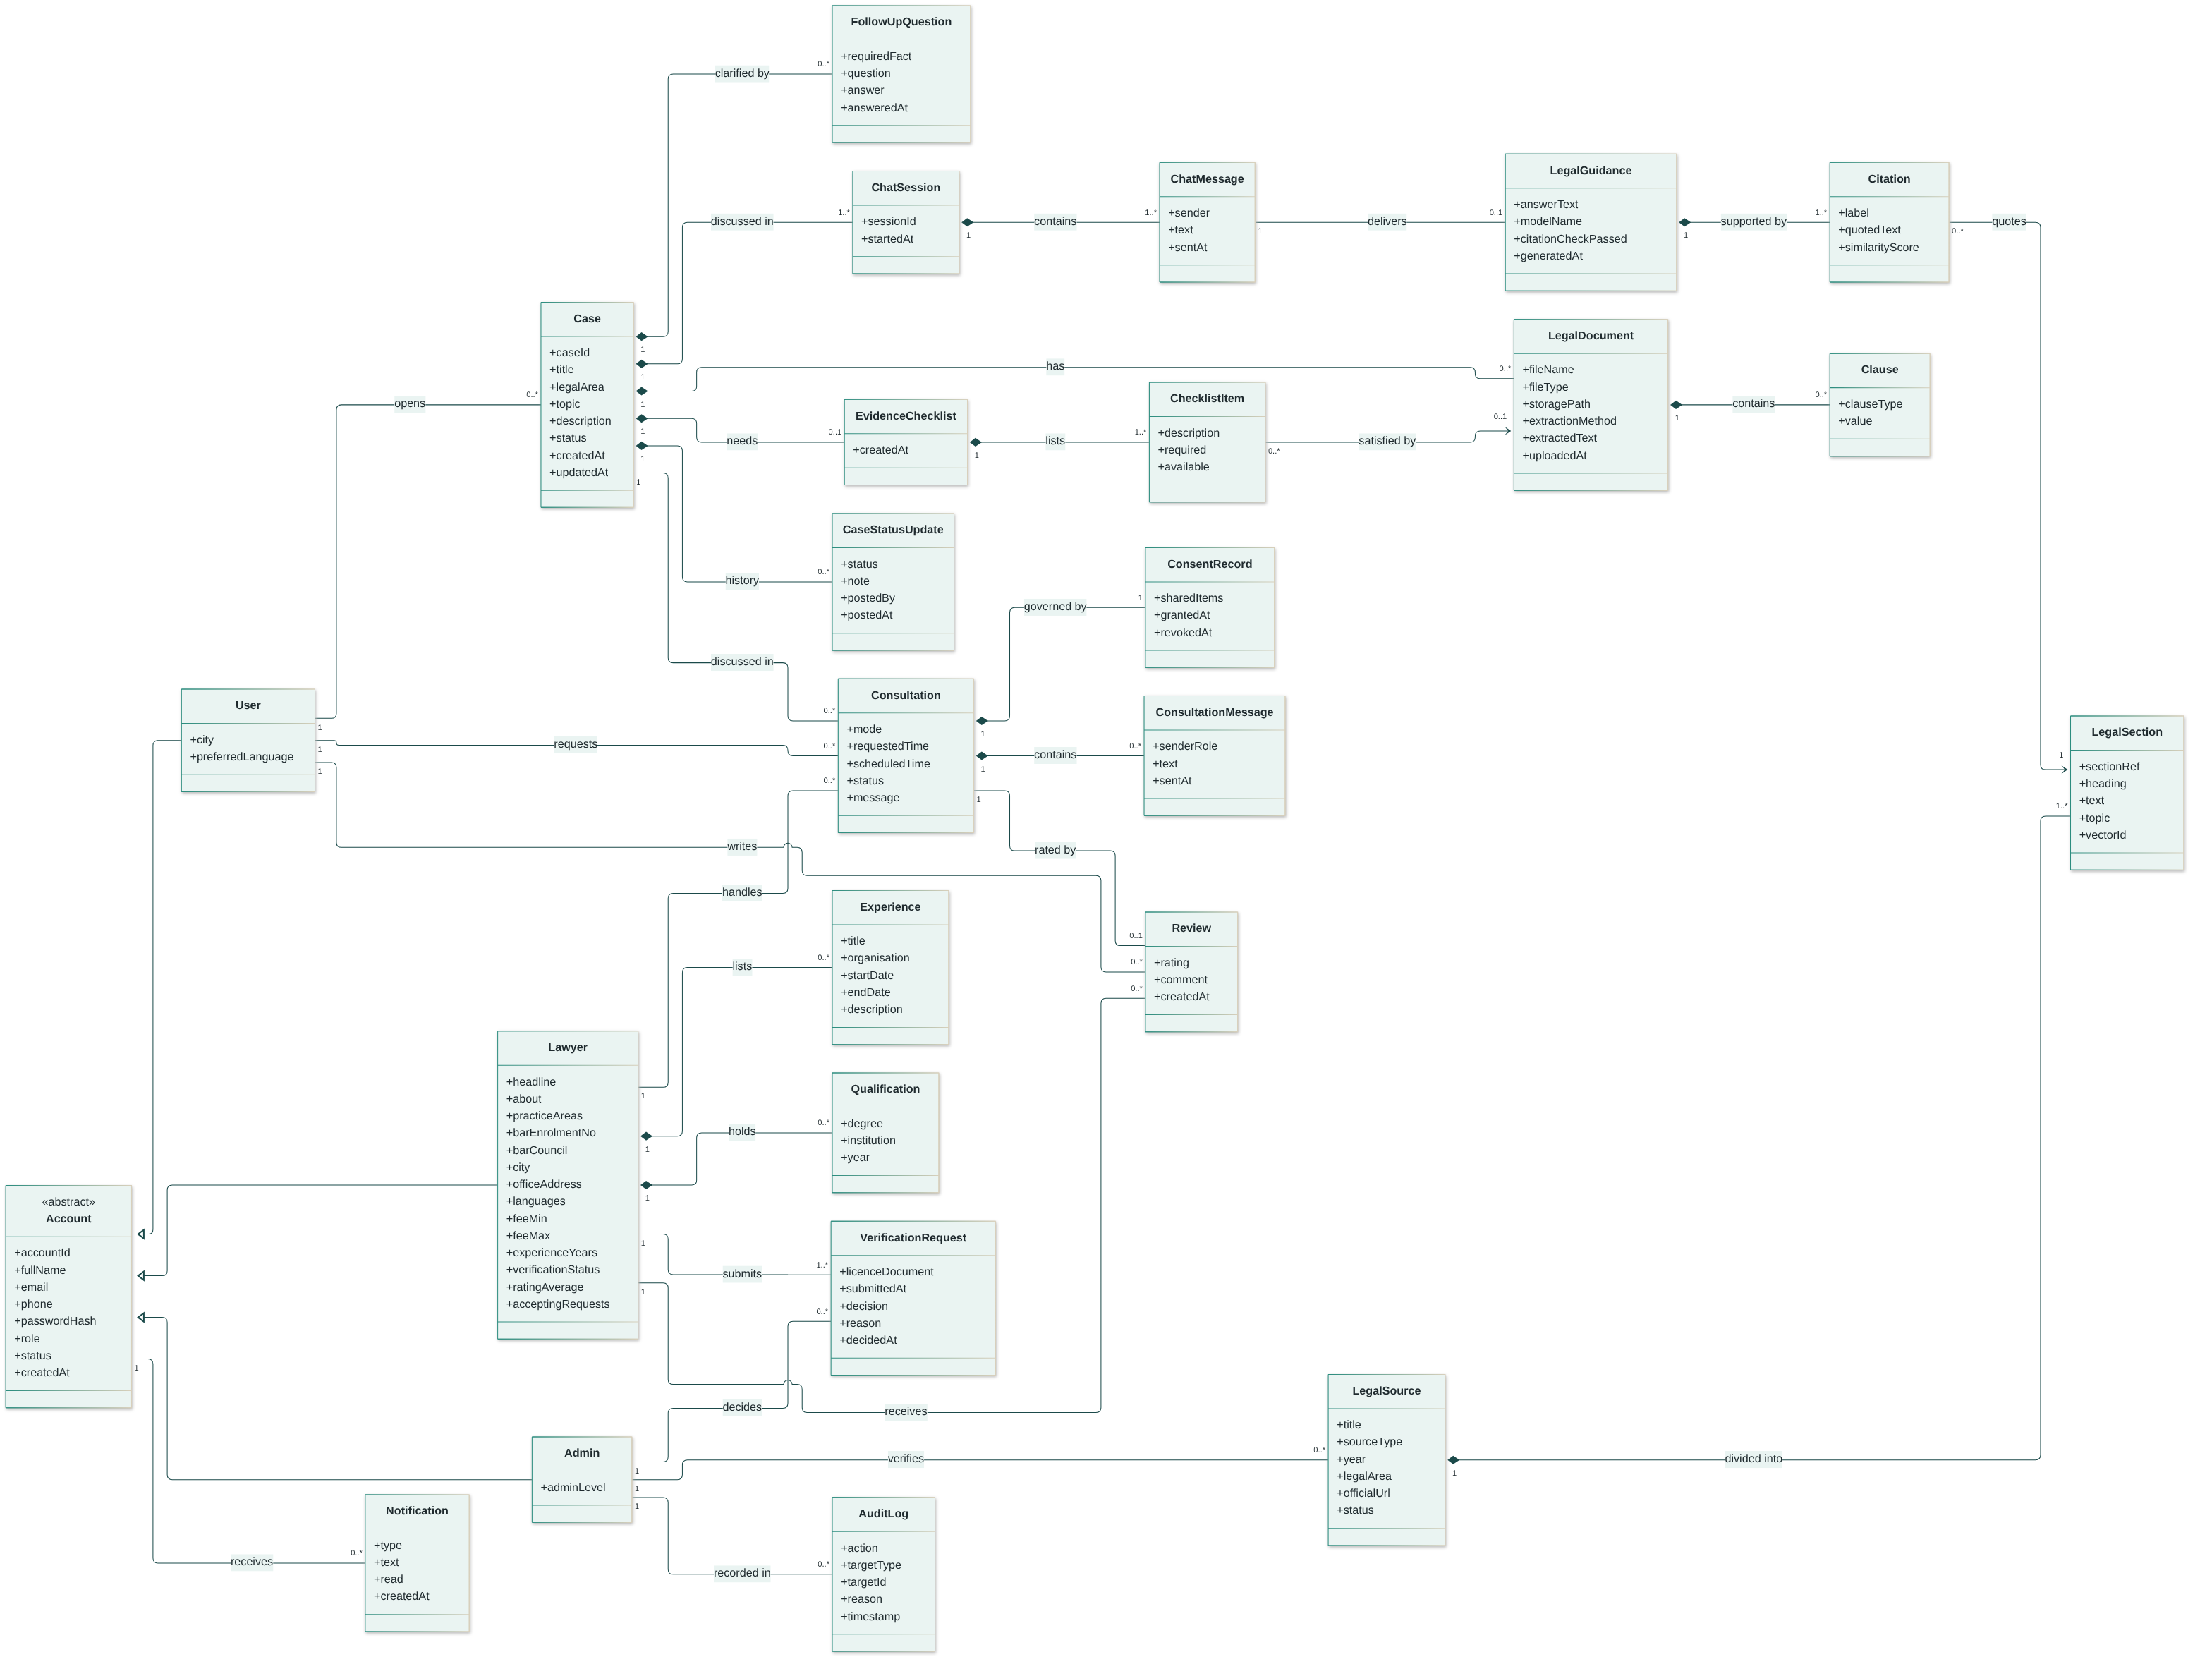
\includegraphics[width=24.5cm,height=14.8cm,keepaspectratio]{figures/domain_model.png}
\caption{Domain model (UML class diagram)}\label{fig:3.12}
\end{figure}
\end{landscape}

\begin{longtable}{|L{3.49cm}|L{8.98cm}|L{2.00cm}|}
\caption{Main entities and their purpose}\label{tab:3.5}\\
\hline\headrow \thd{Entity} & \thd{Purpose} & \thd{Persistence} \\ \hline
\endfirsthead
\hline\headrow \thd{Entity} & \thd{Purpose} & \thd{Persistence} \\ \hline
\endhead
\hline\endlastfoot
Account / User / Lawyer / Admin & Identity, role and role-specific data; \texttt{Lawyer} also holds the public profile. & MongoDB \\ \hline
Experience, Qualification & LinkedIn-style profile sections of a lawyer. & MongoDB (embedded in lawyer) \\ \hline
VerificationRequest & A lawyer's submitted credentials and the Admin's decision. & MongoDB + file store \\ \hline
Case & Central record of a citizen's legal problem and its status. & MongoDB \\ \hline
FollowUpQuestion & A missing fact asked about and the user's answer. & MongoDB \\ \hline
ChatSession, ChatMessage & The conversation between the user and the AI assistant. & MongoDB \\ \hline
LegalGuidance, Citation & An AI answer and the verified references supporting each statement. & MongoDB \\ \hline
LegalSource, LegalSection & Verified statutes, rules and judgments, split into sections. & MongoDB (text, metadata) + Qdrant (embedding) \\ \hline
LegalDocument, Clause & A user's uploaded evidence and the clauses extracted from it. & File store + MongoDB \\ \hline
EvidenceChecklist, ChecklistItem & Case-specific list of documents to prepare. & MongoDB \\ \hline
Consultation, ConsentRecord, ConsultationMessage & A user-lawyer engagement, what the user agreed to share, and the messages exchanged. & MongoDB \\ \hline
CaseStatusUpdate & Timeline entries posted by the user, lawyer or system. & MongoDB \\ \hline
Review & Rating and comment after a completed consultation. & MongoDB \\ \hline
Notification, AuditLog & User alerts and a record of administrative actions. & MongoDB \\
\end{longtable}

\textbf{Key cardinalities explained.}

\begin{itemize}
  \item A \textbf{User} may open many \textbf{Cases} (1 to 0..*), but each case belongs to exactly one user.
  \item A \textbf{Case} is discussed in one or more \textbf{ChatSessions}. Each assistant message may deliver at most one \textbf{LegalGuidance}, and every guidance must have at least one \textbf{Citation} (1..*). This enforces the rule that no unsupported answer is stored.
  \item Each \textbf{Citation} quotes exactly one \textbf{LegalSection}, and a section may be cited by many answers.
  \item A \textbf{Consultation} links one user, one lawyer and one case, and is governed by exactly one \textbf{ConsentRecord}. Users and lawyers are thereby connected many-to-many through consultations.
  \item A \textbf{Consultation} can receive at most one \textbf{Review}, which prevents duplicate reviews of the same engagement.
\end{itemize}

\needspace{12\baselineskip}
\section{User Interface Design (Prototypes)}

The interfaces follow five design principles derived from the requirements:

\begin{enumerate}
  \item \textbf{Plain language first:} labels and guidance avoid unexplained legal terms (NFR-USA-03).
  \item \textbf{Proof is visible:} every guidance statement shows a source tag that opens the cited law (UFR-11).
  \item \textbf{Ask, don't assume:} missing facts are requested through short questions, and the facts collected so far are always shown (UFR-08).
  \item \textbf{Consent before sharing:} the user sees exactly what a lawyer will receive (UFR-25).
  \item \textbf{One consistent layout:} all three portals use the same sidebar navigation, colour palette (dark teal with gold accents) and components, and are responsive (NFR-USA-03).
\end{enumerate}

High-fidelity prototypes of the core screens were produced as a clickable HTML prototype. Screens marked ``To be prototyped'' are specified here and will be designed in the next iteration.

% Mermaid source:
% flowchart TD
%     L["Login / Register"] --> UD["User Dashboard"]
%     L --> LD["Lawyer Dashboard"]
%     L --> AD["Admin Dashboard"]
%     UD --> NC["New Case"] --> FQ["Follow-up Questions"] --> GD["AI Guidance + Sources"]
%     GD --> DC["Documents + Checklist"]
%     GD --> DIR["Lawyer Directory"] --> PP["Public Lawyer Profile"] --> CR["Consultation Request + Consent"]
%     UD --> TR["Case Tracking Timeline"]
%     CR --> TR
%     LD --> REQ["Consultation Requests"] --> SC["Shared Case View"] --> UPD["Post Update / Message"]
%     LD --> PE["Profile Editor + Verification"]
%     AD --> VQ["Lawyer Verification Queue"]
%     AD --> UM["User and Lawyer Management"]
%     AD --> KB["Legal Knowledge Base"]
%     AD --> AL["Audit Log and Reports"]
\begin{figure}[H]\centering
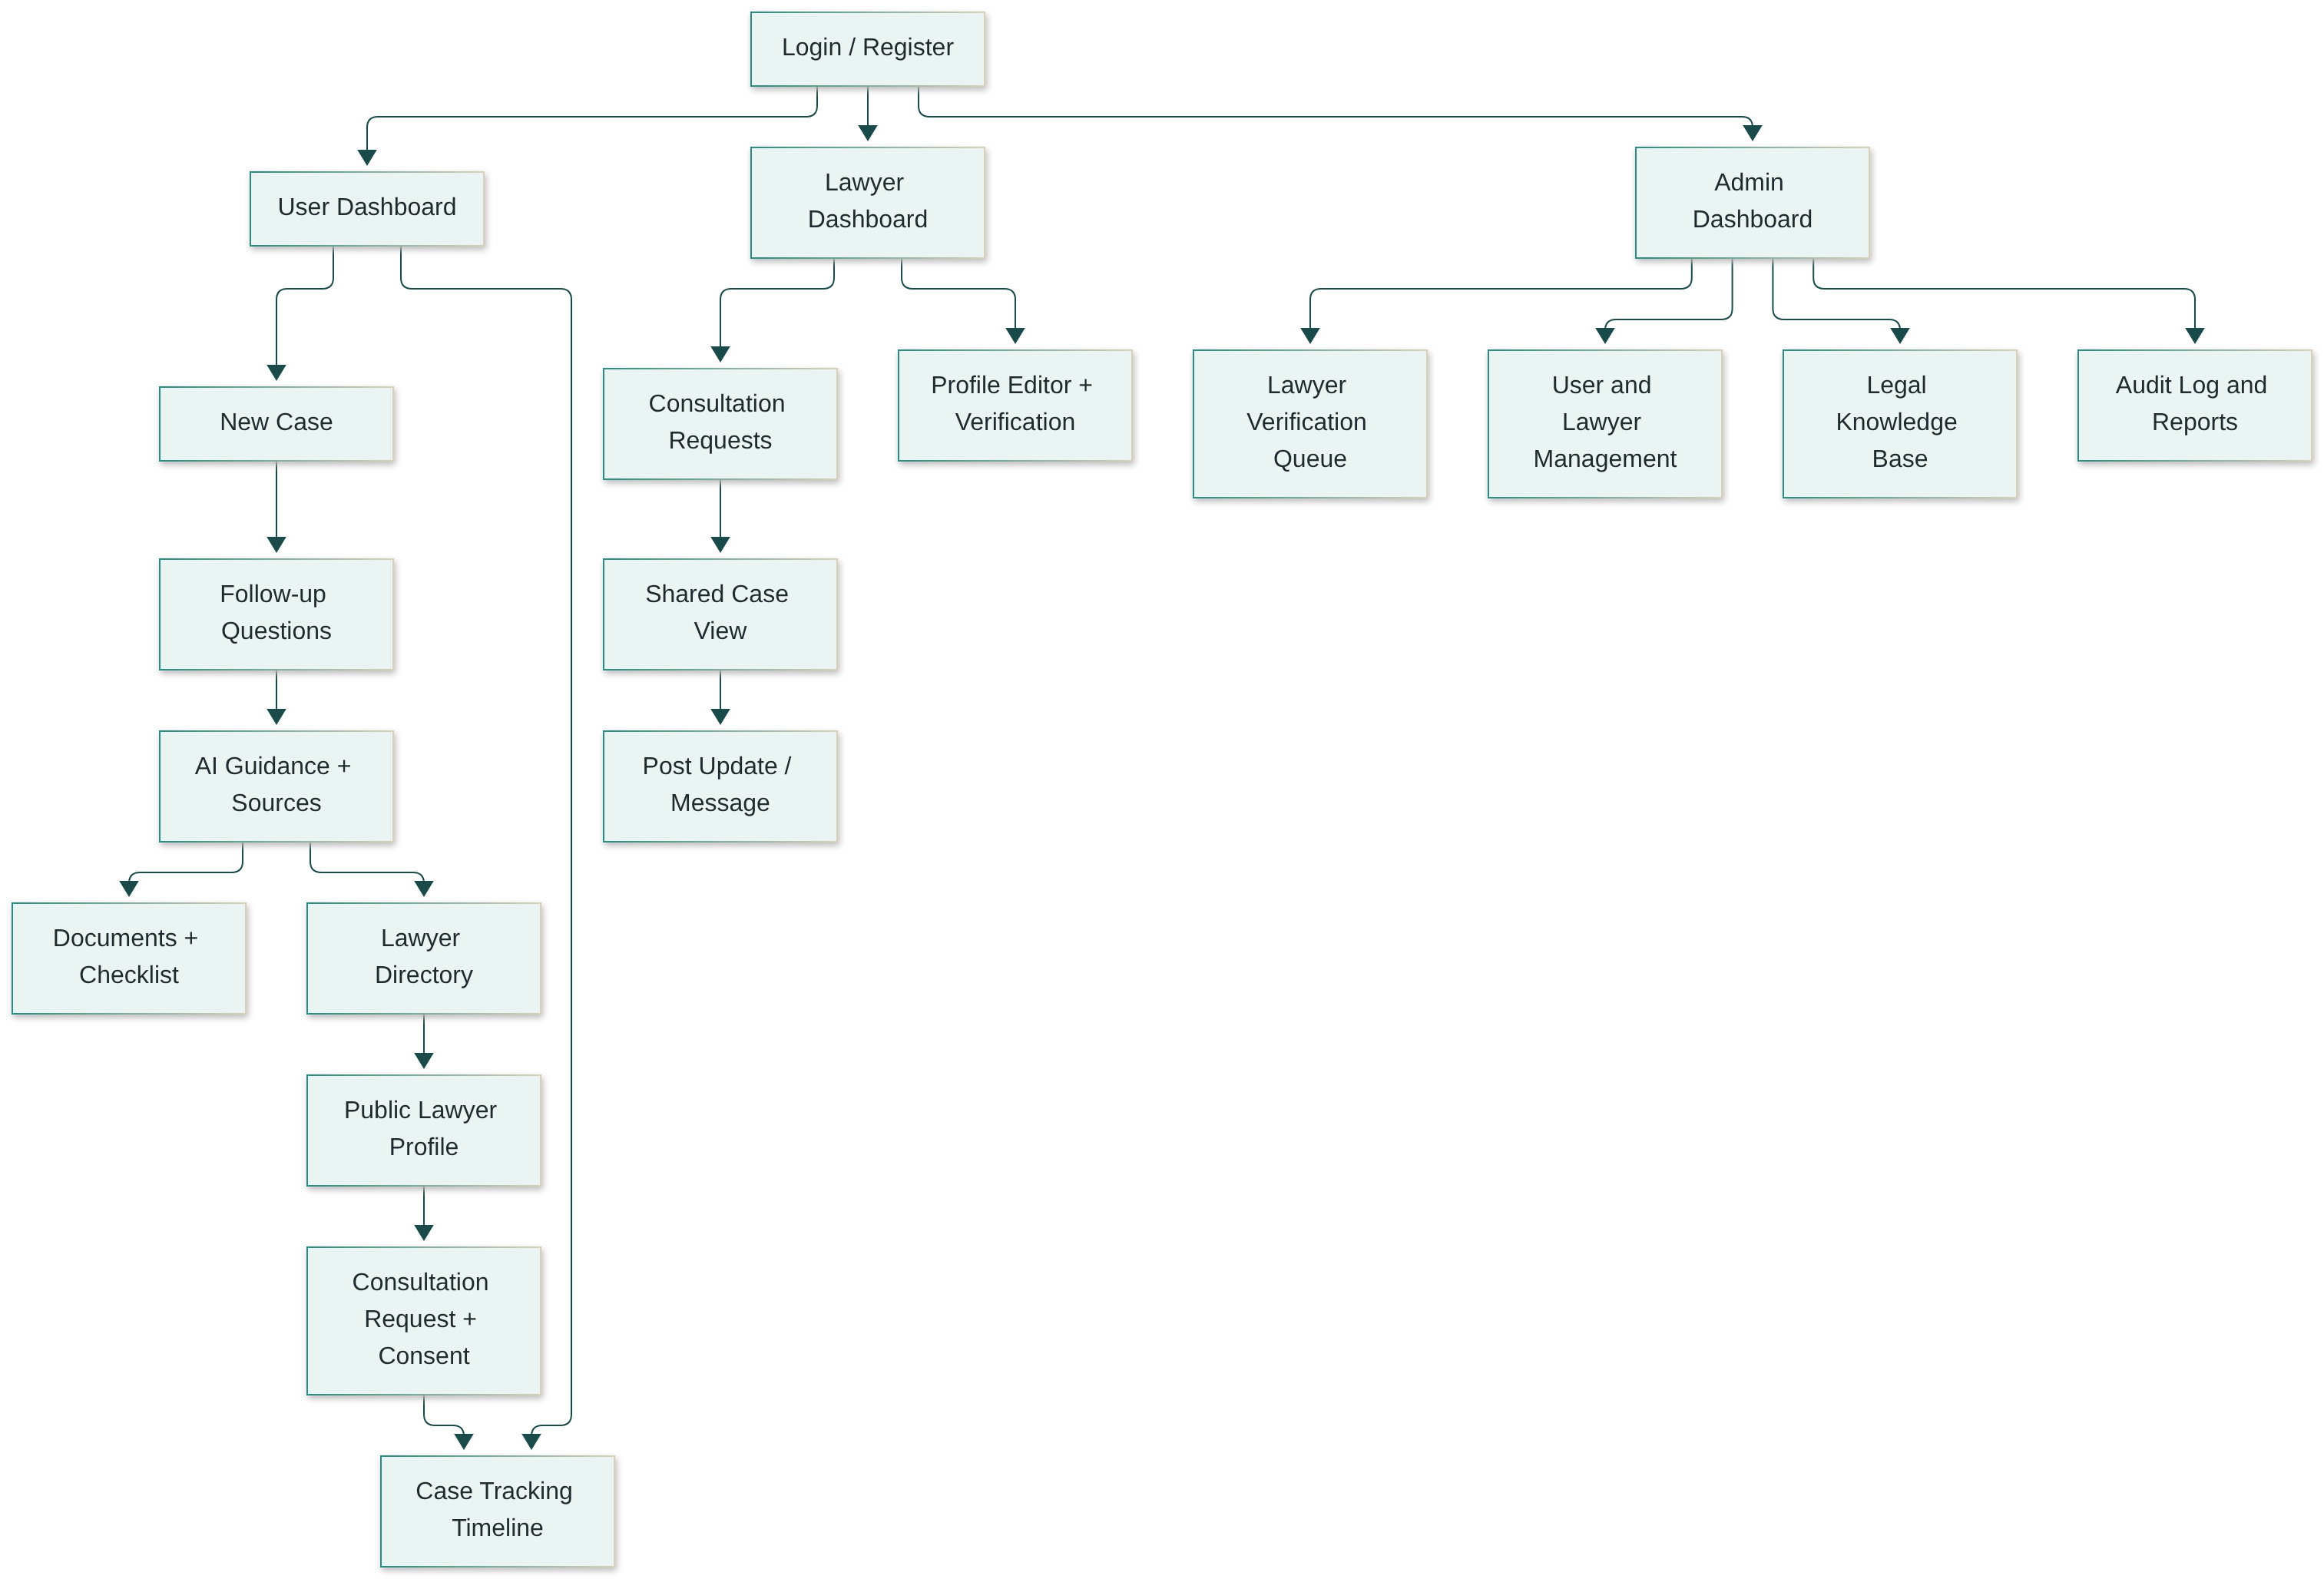
\includegraphics[width=\textwidth,height=0.62\textheight,keepaspectratio]{figures/nav_map.png}
\caption{Portal navigation map}\label{fig:3.13}
\end{figure}

\needspace{12\baselineskip}
\subsection{Authentication Screens}

\begin{center}
\begin{tabular}{|L{1.70cm}|L{8.39cm}|L{1.82cm}|L{2.10cm}|}
\hline\headrow \thd{Screen} & \thd{Purpose and key elements} & \thd{Requirements} & \thd{Status} \\ \hline
Sign in & Role selector (User, Lawyer, Admin), email, password, ``Forgot password'', link to register. A side panel explains the platform and the disclaimer. & UFR-02, LFR-02, AFR-01 & Prototyped (Figure~\ref{fig:3.14}) \\ \hline
Register & Role-specific form; lawyers also enter bar enrolment number, bar council and upload the licence. & UFR-01, LFR-01 & To be prototyped \\ \hline
Reset password & Email entry, then a new-password form from the emailed link. & UFR-03 & To be prototyped \\ \hline
\end{tabular}
\end{center}

\begin{figure}[H]\centering
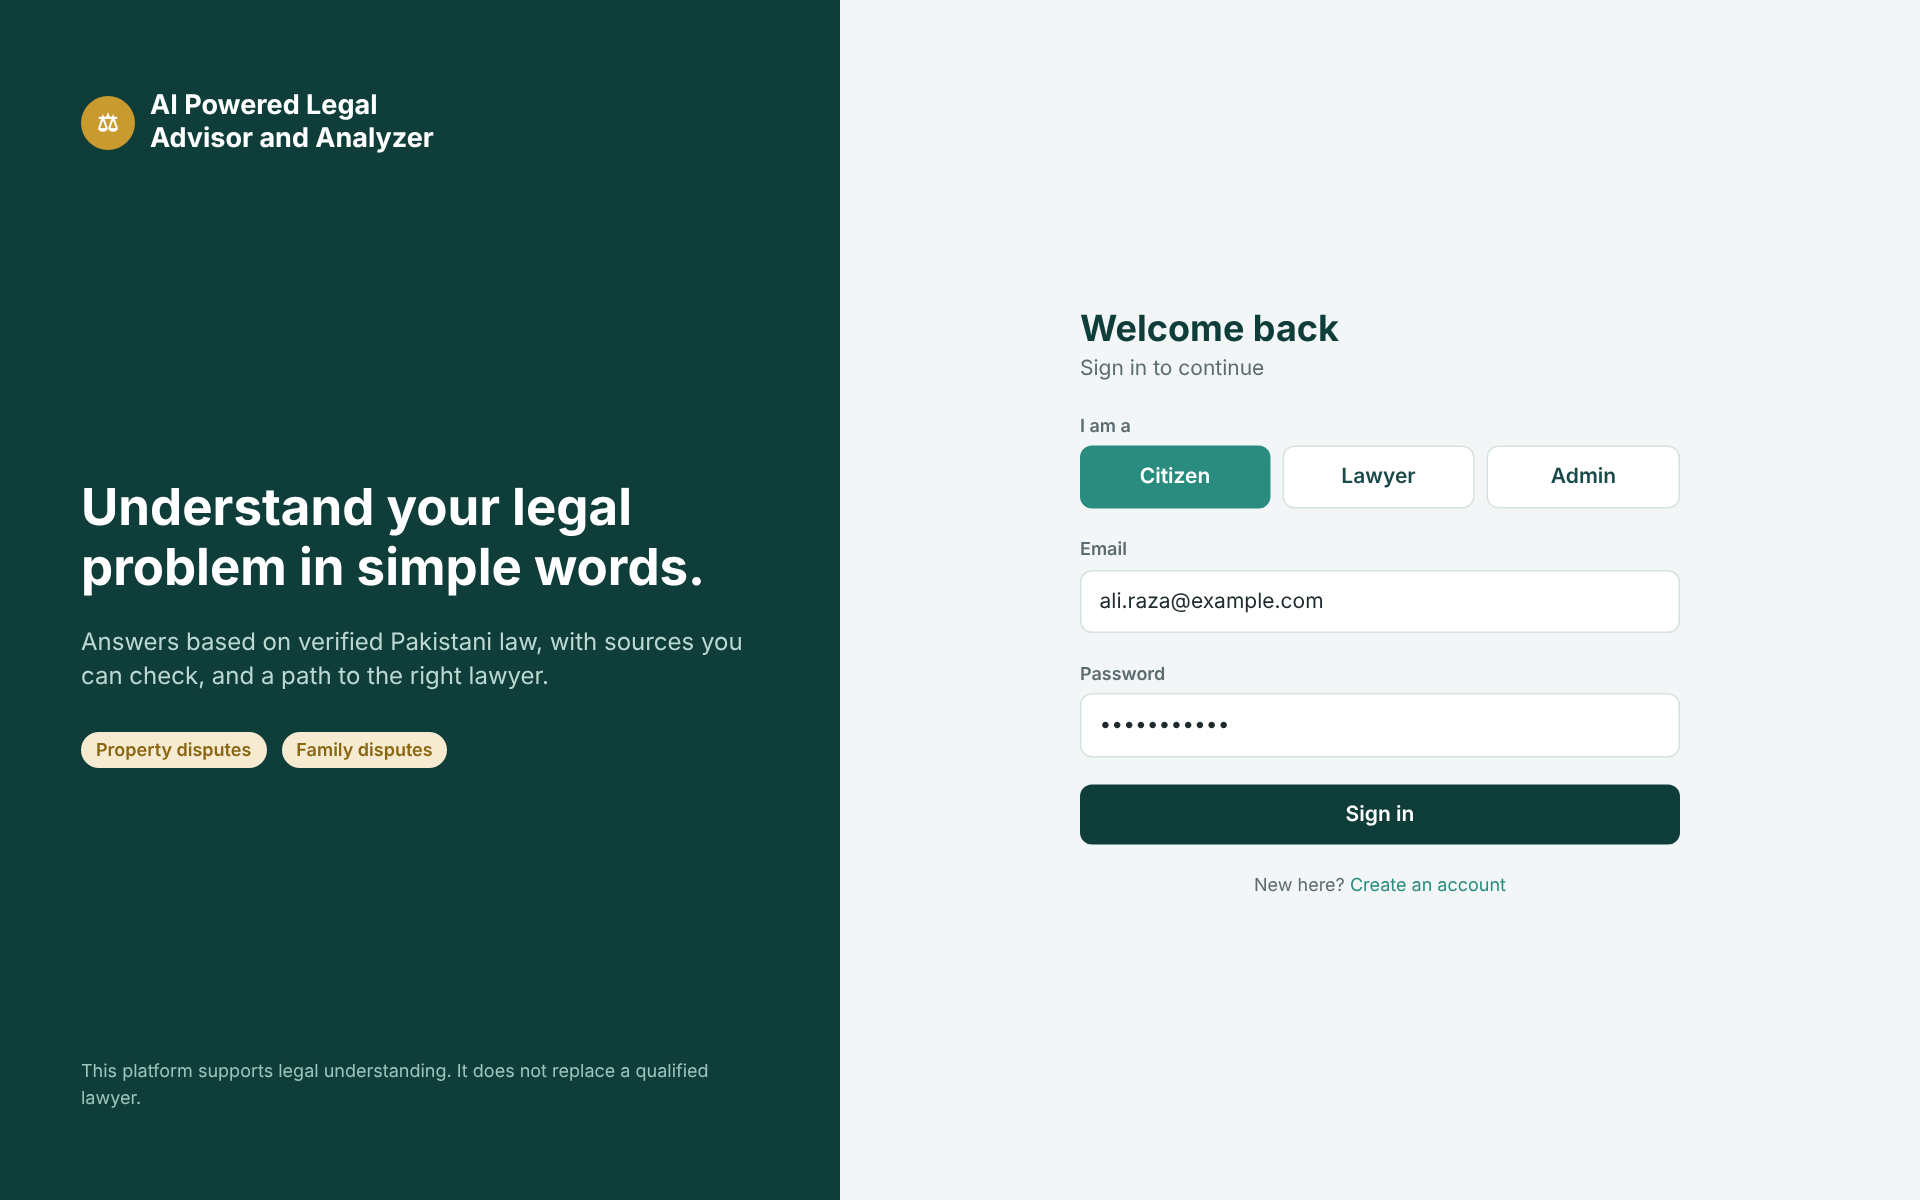
\includegraphics[width=\textwidth,height=0.62\textheight,keepaspectratio]{figures/screens/01_login.png}
\caption{Sign-in screen with role selection}\label{fig:3.14}
\end{figure}

\needspace{12\baselineskip}
\subsection{User Portal}

\begin{longtable}{|L{2.01cm}|L{7.10cm}|L{1.70cm}|L{3.20cm}|}
\hline\headrow \thd{Screen} & \thd{Purpose and key elements} & \thd{Requirements} & \thd{Status} \\ \hline
\endfirsthead
\hline\headrow \thd{Screen} & \thd{Purpose and key elements} & \thd{Requirements} & \thd{Status} \\ \hline
\endhead
\hline\endlastfoot
User dashboard & Summary cards (open cases, cases needing an answer, shared cases), ``New case'' button, recent cases table with area and status. & UFR-16, UFR-29 & Prototyped (Figure~\ref{fig:3.15}) \\ \hline
New case & Title and free-text description, optional document attachment, detected legal area and topic with ``Change area''. & UFR-06, UFR-07 & Prototyped (Figure~\ref{fig:3.16}) \\ \hline
AI chat / follow-up questions & Chat view with the user's messages and the assistant's numbered follow-up questions; side panel ``Facts so far'' with completed and missing facts. & UFR-08, UFR-15 & Prototyped (Figure~\ref{fig:3.17}) \\ \hline
AI legal guidance & Plain-language answer with inline source tags, sources table (law, section, match), disclaimer, evidence checklist with progress bar, and ``Find a lawyer'' call to action. & UFR-10 to UFR-14, UFR-20 & Prototyped (Figure~\ref{fig:3.18}) \\ \hline
Documents & Drag-and-drop upload, file list with extraction method (PyMuPDF/OCR) and status, extracted key clauses. & UFR-17 to UFR-19 & Prototyped (Figure~\ref{fig:3.19}) \\ \hline
Lawyer directory & Filter panel (specialisation, city, fee, experience, language, rating) and result cards with verified badge, rating and fee range. & UFR-22 & Prototyped (Figure~\ref{fig:3.20}) \\ \hline
Public lawyer profile & Professional-network-style page: photo, headline, verified badge, about, practice areas, experience timeline, education, languages, fee range, reviews and ``Request consultation''. & UFR-23 & Header and consent dialog prototyped (Figure~\ref{fig:3.21}); full profile body to be prototyped \\ \hline
Consultation request and consent & Form for case, mode, preferred time and message, followed by a consent dialog listing the shared items. & UFR-24, UFR-25 & Consent dialog prototyped (Figure~\ref{fig:3.21}) \\ \hline
Case tracking & Case header with status, vertical timeline of events and lawyer updates, assigned lawyer card, checklist progress, ``Stop sharing''. & UFR-26, UFR-29 & Prototyped (Figure~\ref{fig:3.22}) \\ \hline
Consultation messages & Message thread with the lawyer inside an accepted consultation. & UFR-27 & To be prototyped \\ \hline
Profile and settings & Personal details, password change, notification preferences, account deletion. & UFR-04, UFR-05, UFR-30 & To be prototyped \\
\end{longtable}

\begin{figure}[H]\centering
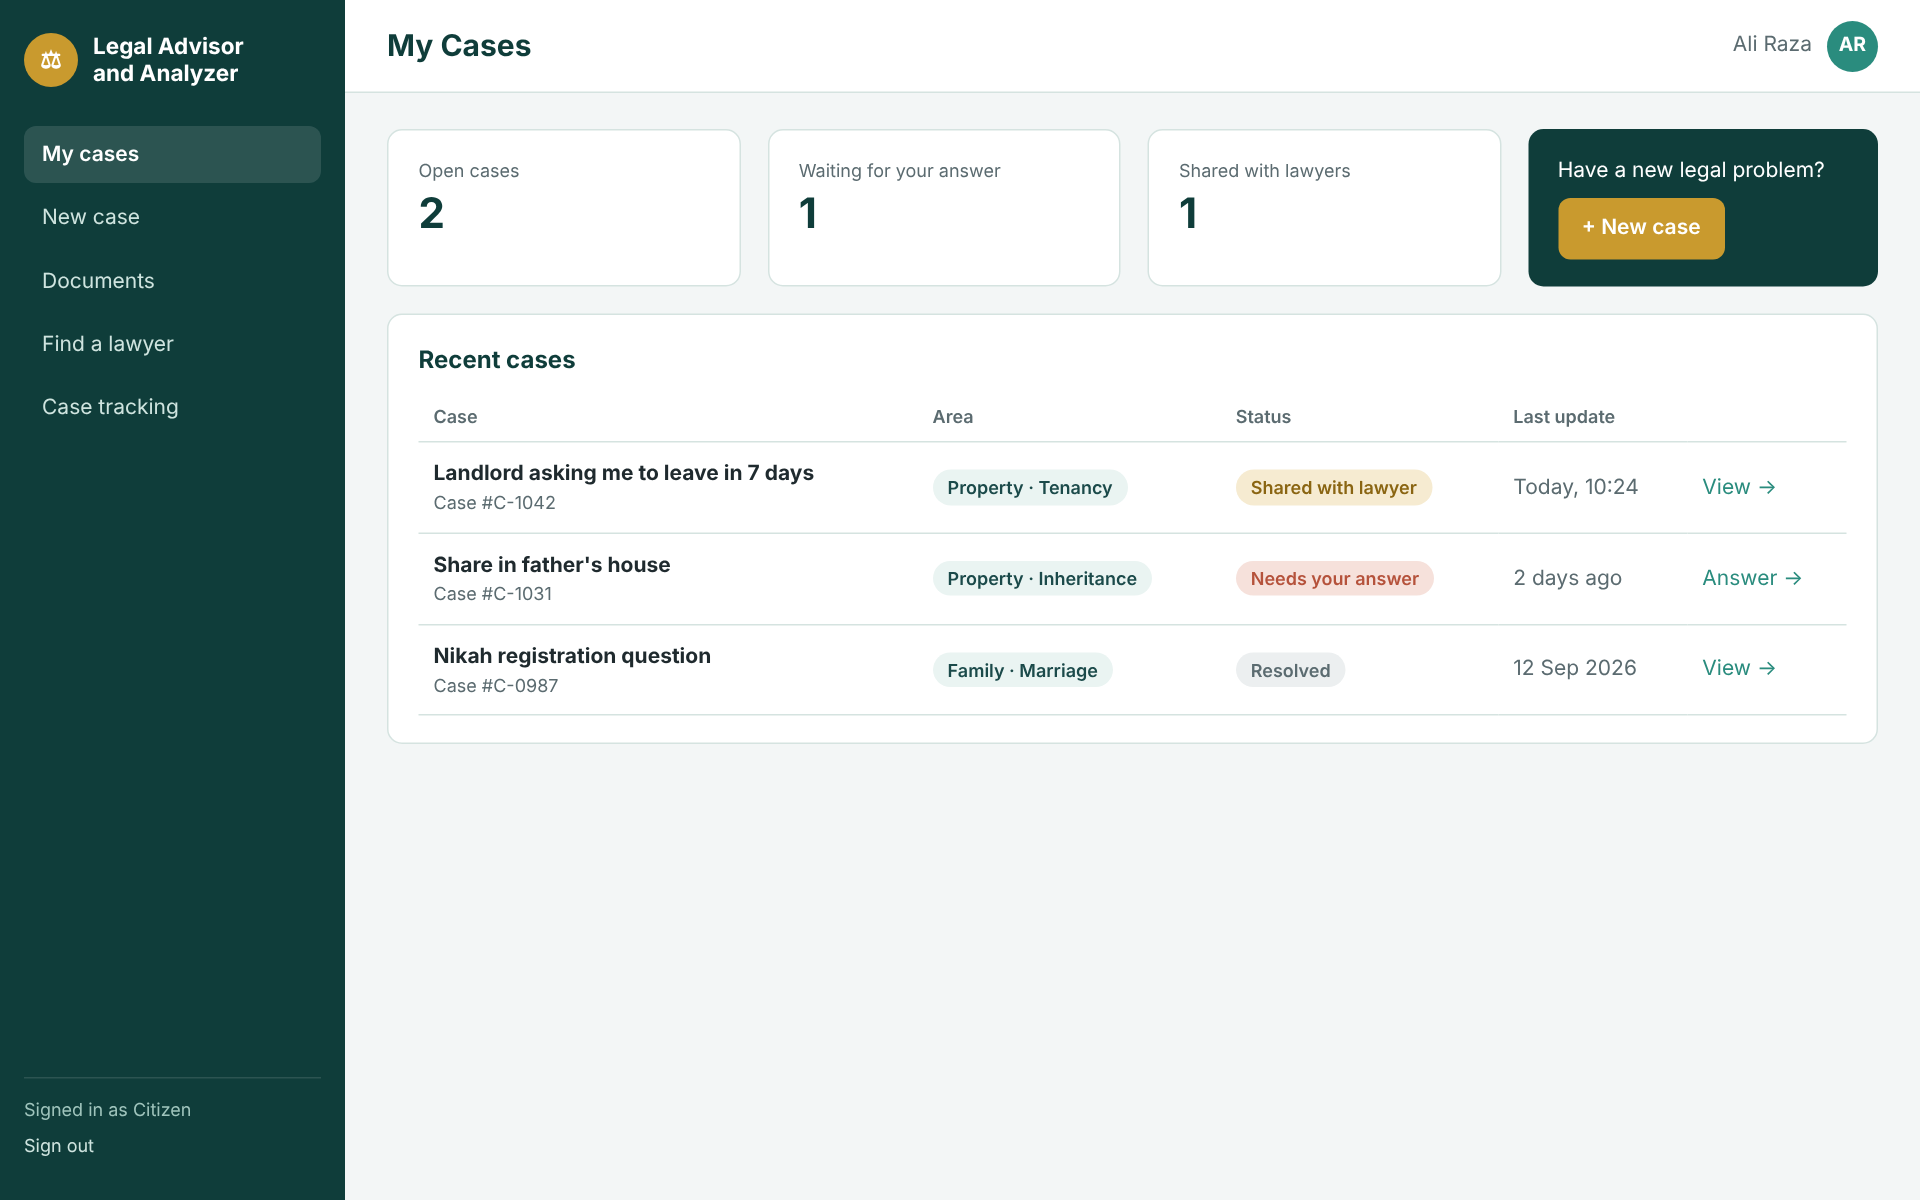
\includegraphics[width=\textwidth,height=0.62\textheight,keepaspectratio]{figures/screens/02_dashboard.png}
\caption{User dashboard}\label{fig:3.15}
\end{figure}

\begin{figure}[H]\centering
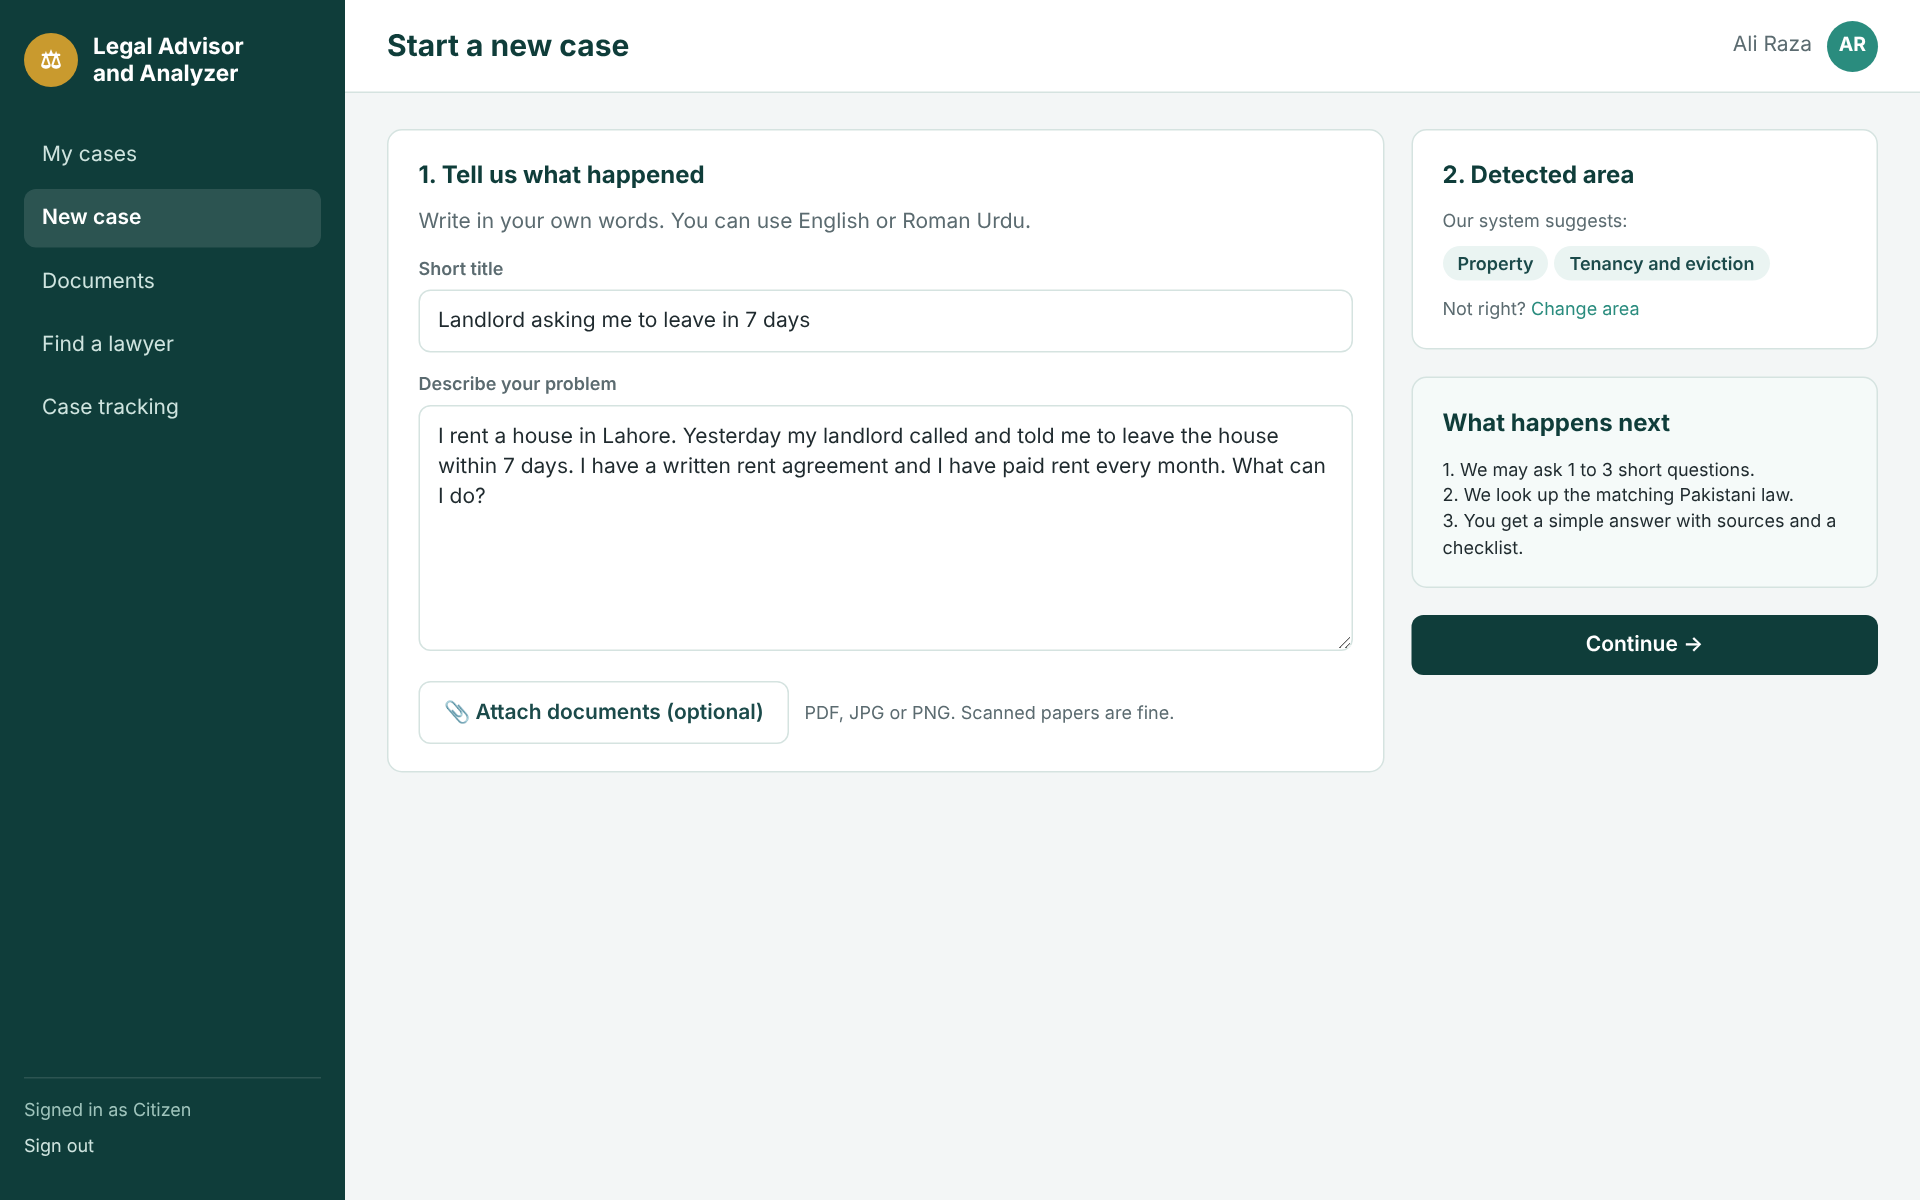
\includegraphics[width=\textwidth,height=0.62\textheight,keepaspectratio]{figures/screens/03_newcase.png}
\caption{New case screen}\label{fig:3.16}
\end{figure}

\begin{figure}[H]\centering
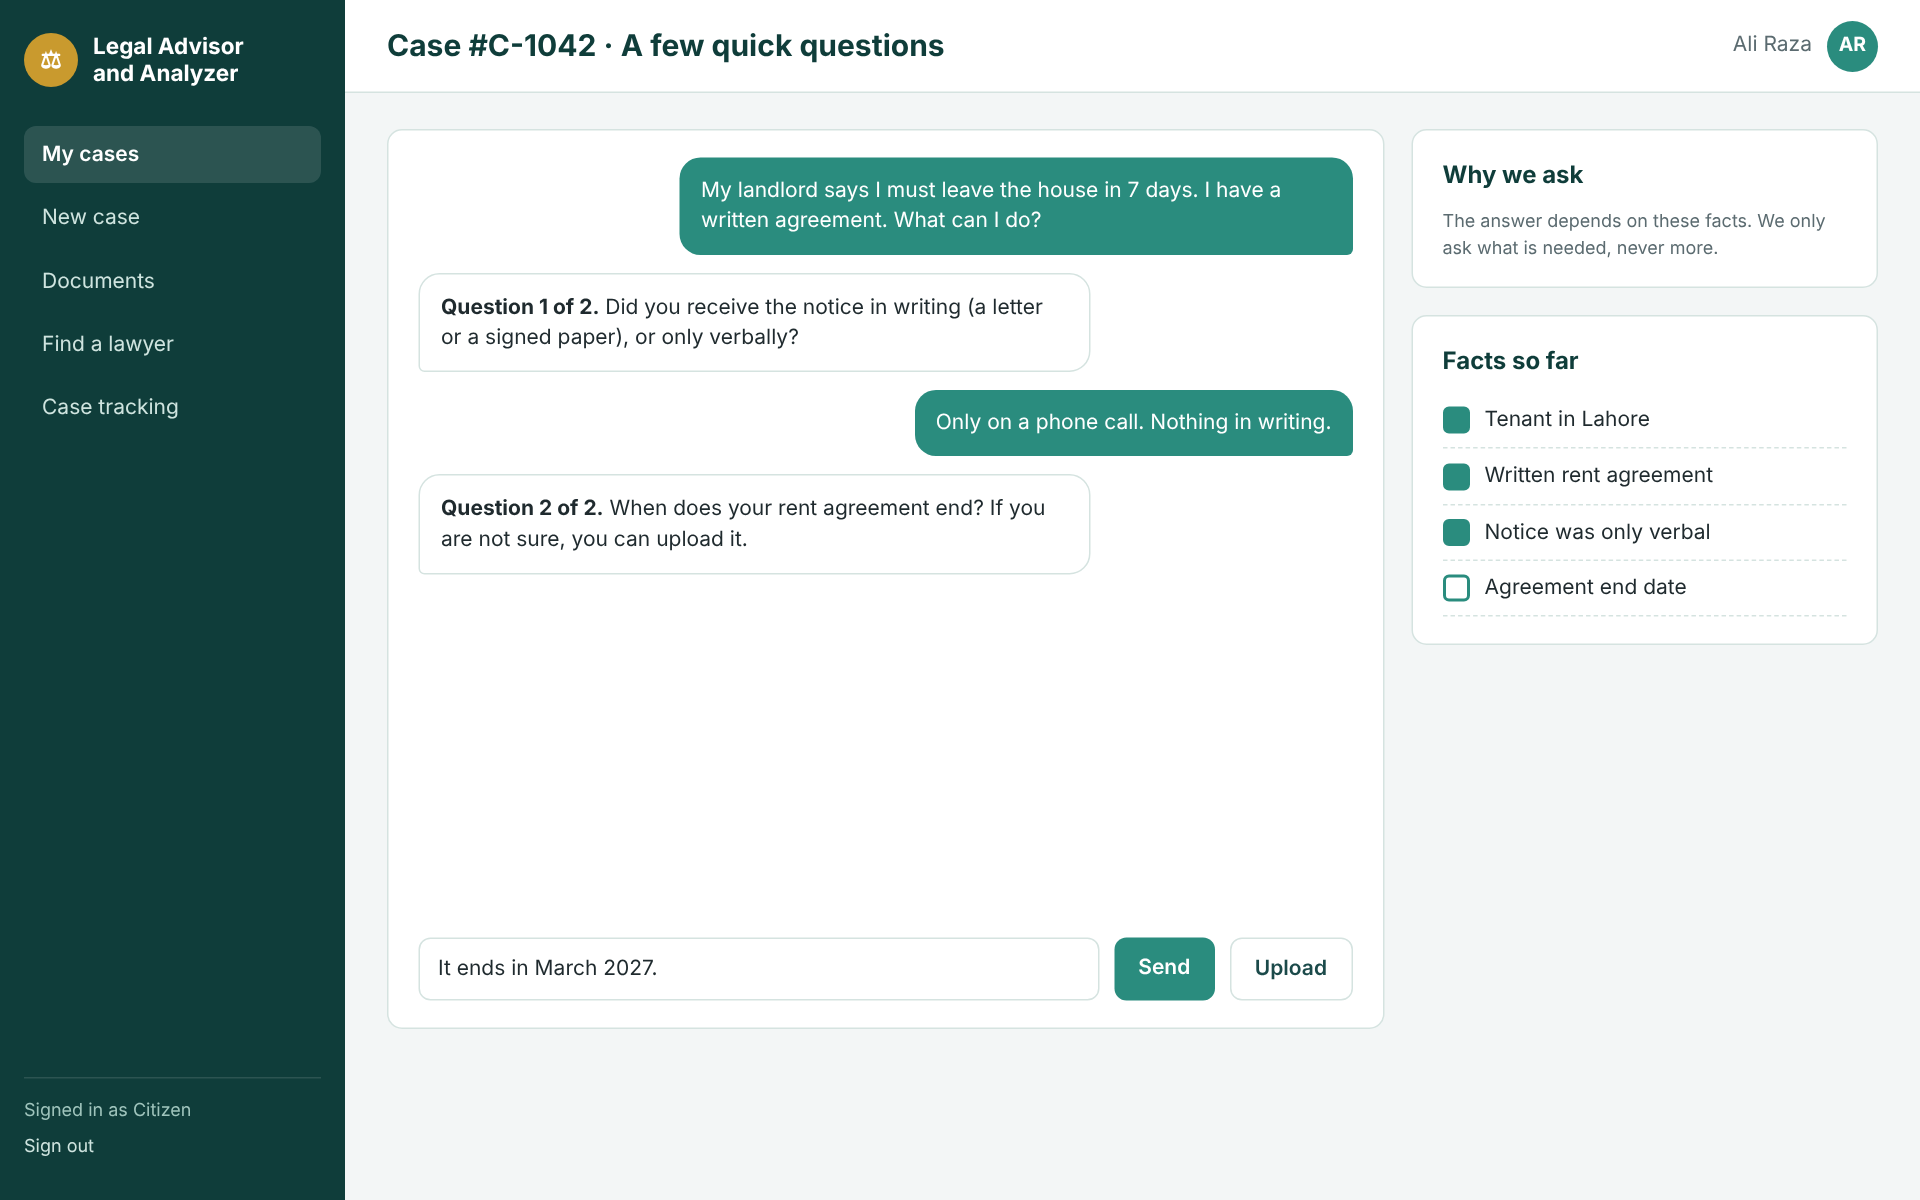
\includegraphics[width=\textwidth,height=0.62\textheight,keepaspectratio]{figures/screens/04_followup.png}
\caption{AI chat with follow-up questions}\label{fig:3.17}
\end{figure}

\begin{figure}[H]\centering
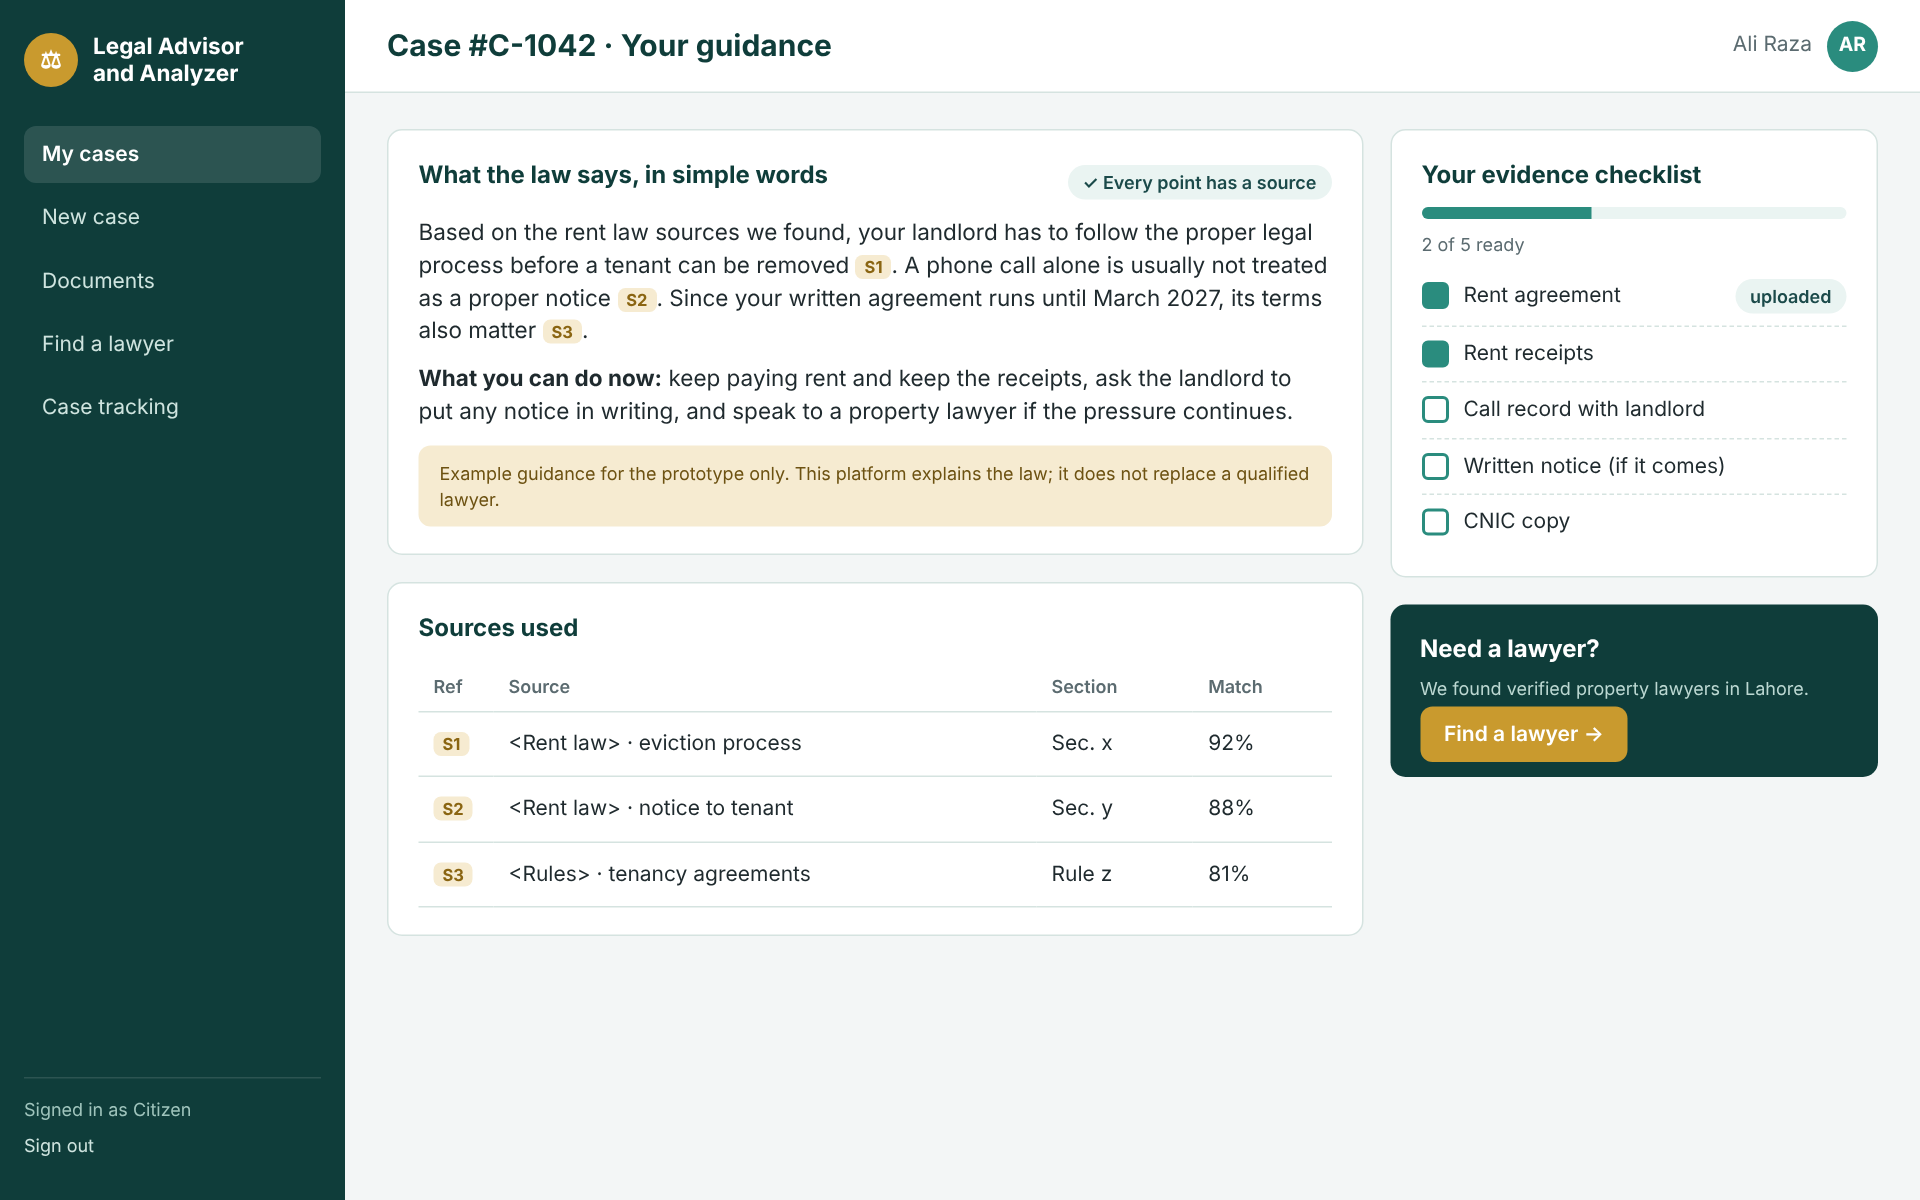
\includegraphics[width=\textwidth,height=0.62\textheight,keepaspectratio]{figures/screens/05_guidance.png}
\caption{AI legal guidance with sources and evidence checklist}\label{fig:3.18}
\end{figure}

\begin{figure}[H]\centering
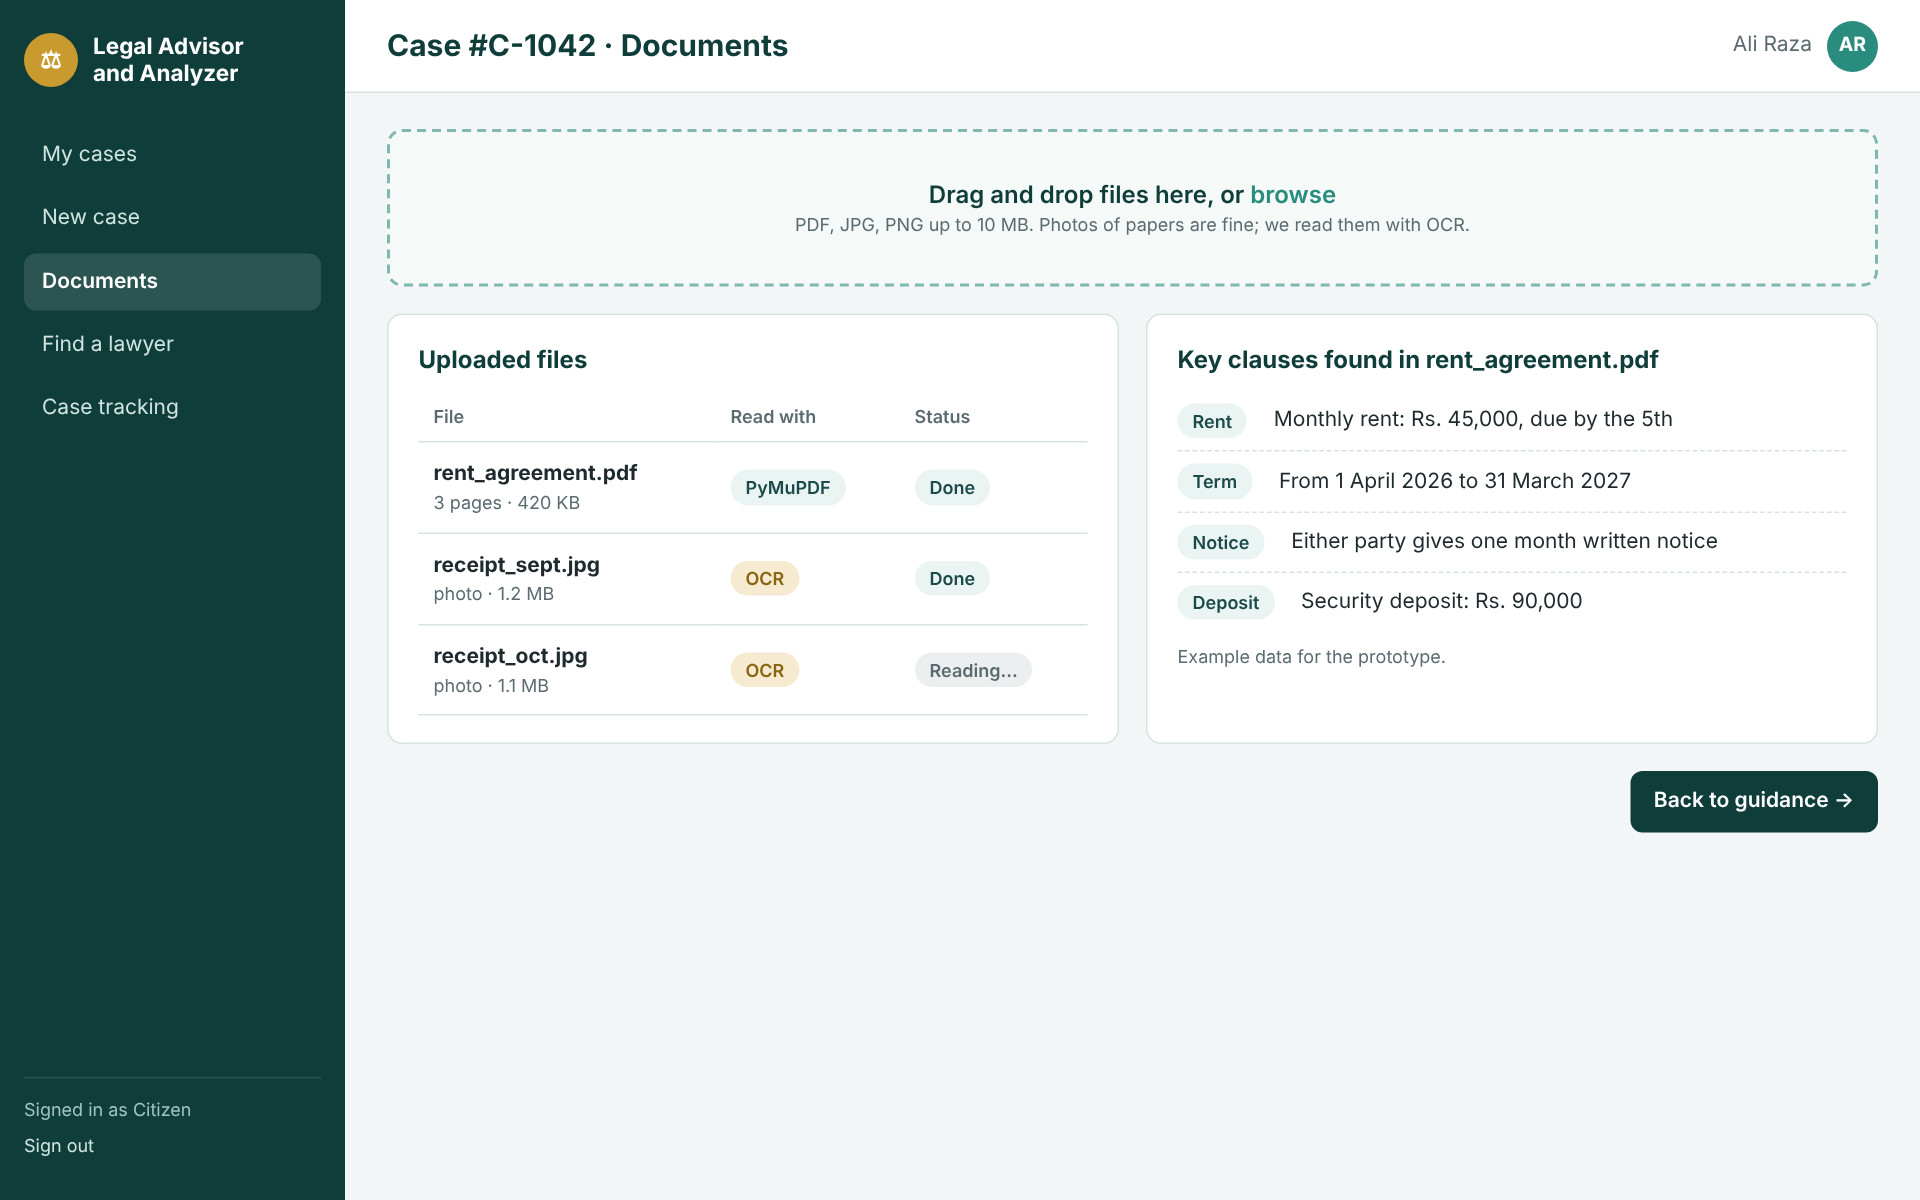
\includegraphics[width=\textwidth,height=0.62\textheight,keepaspectratio]{figures/screens/06_documents.png}
\caption{Document upload and clause extraction}\label{fig:3.19}
\end{figure}

\begin{figure}[H]\centering
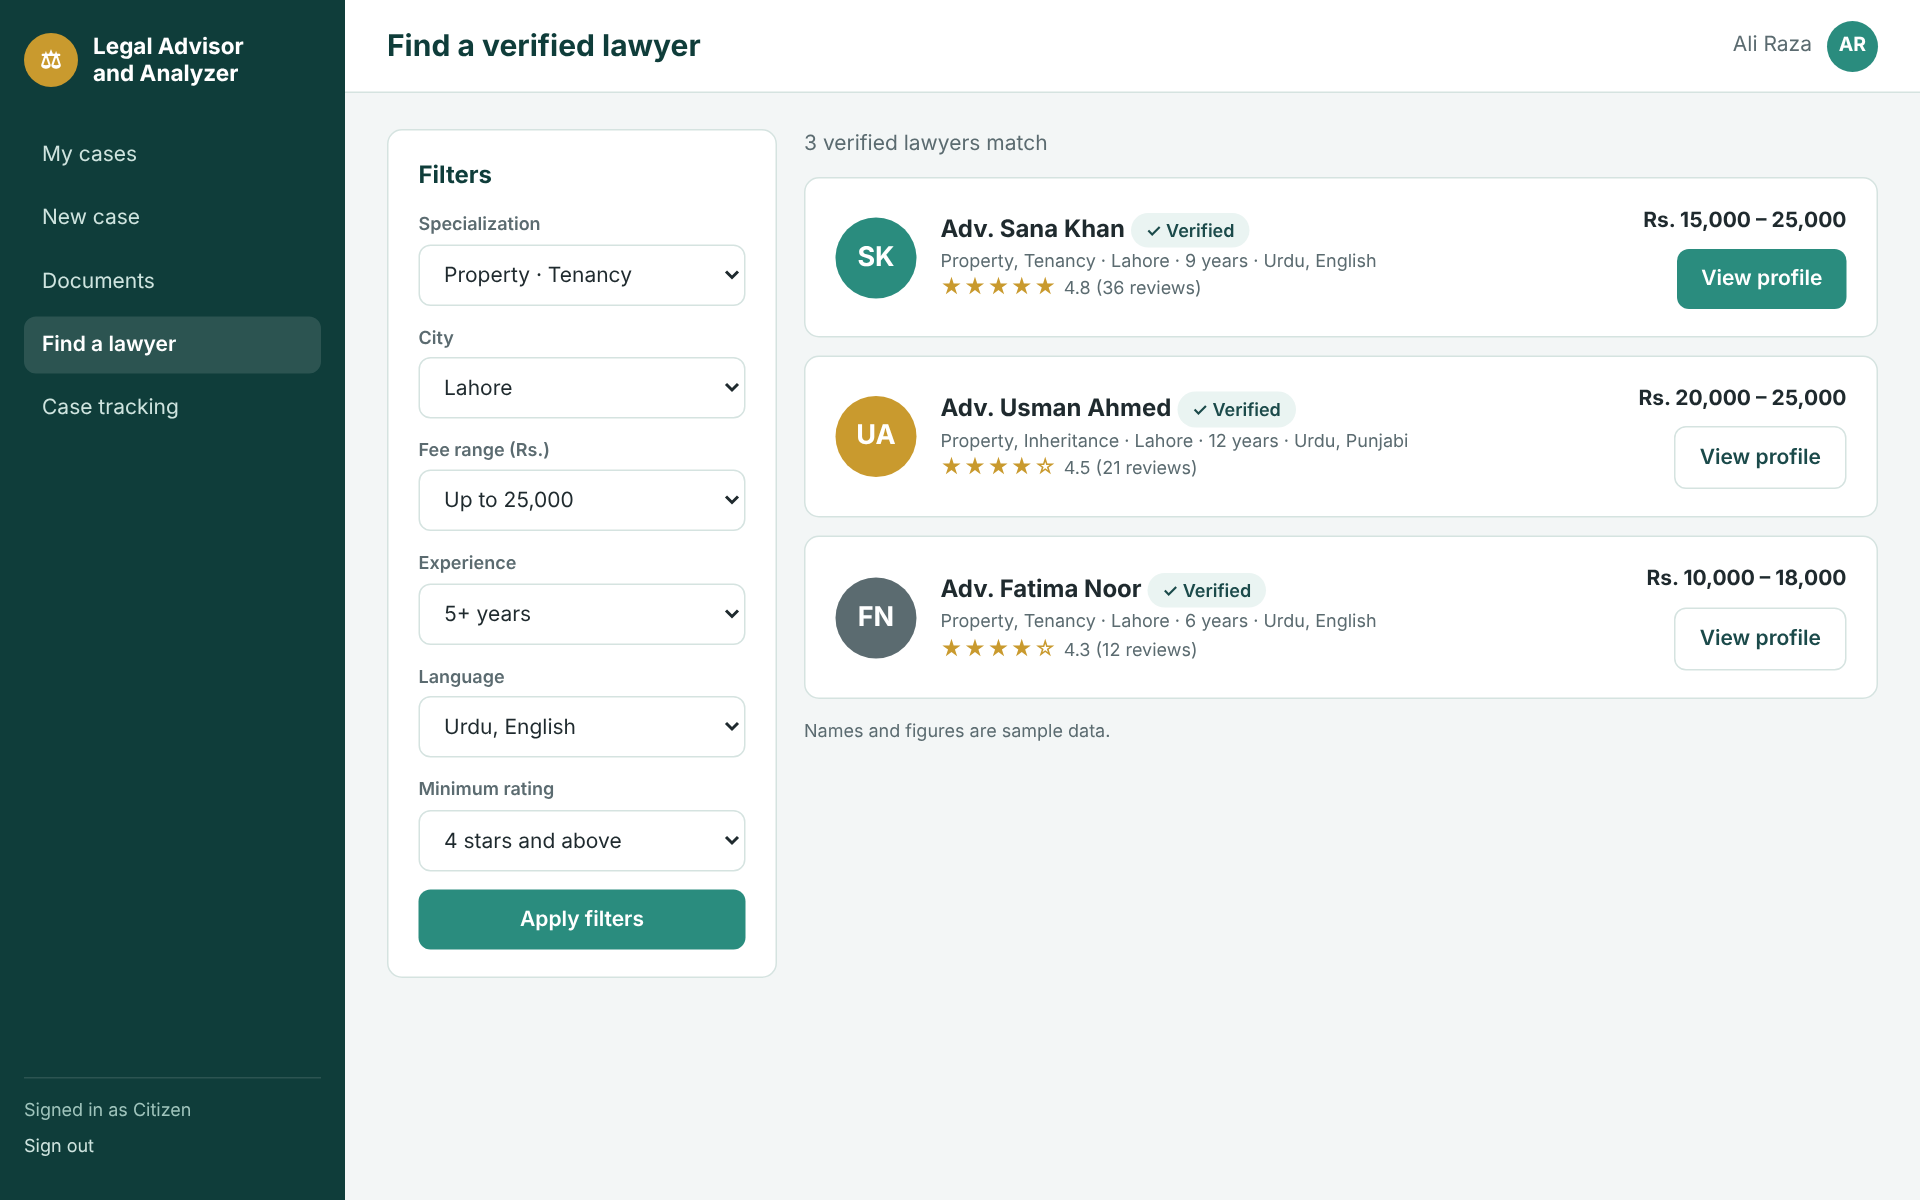
\includegraphics[width=\textwidth,height=0.62\textheight,keepaspectratio]{figures/screens/07_directory.png}
\caption{Lawyer directory with filters}\label{fig:3.20}
\end{figure}

\begin{figure}[H]\centering
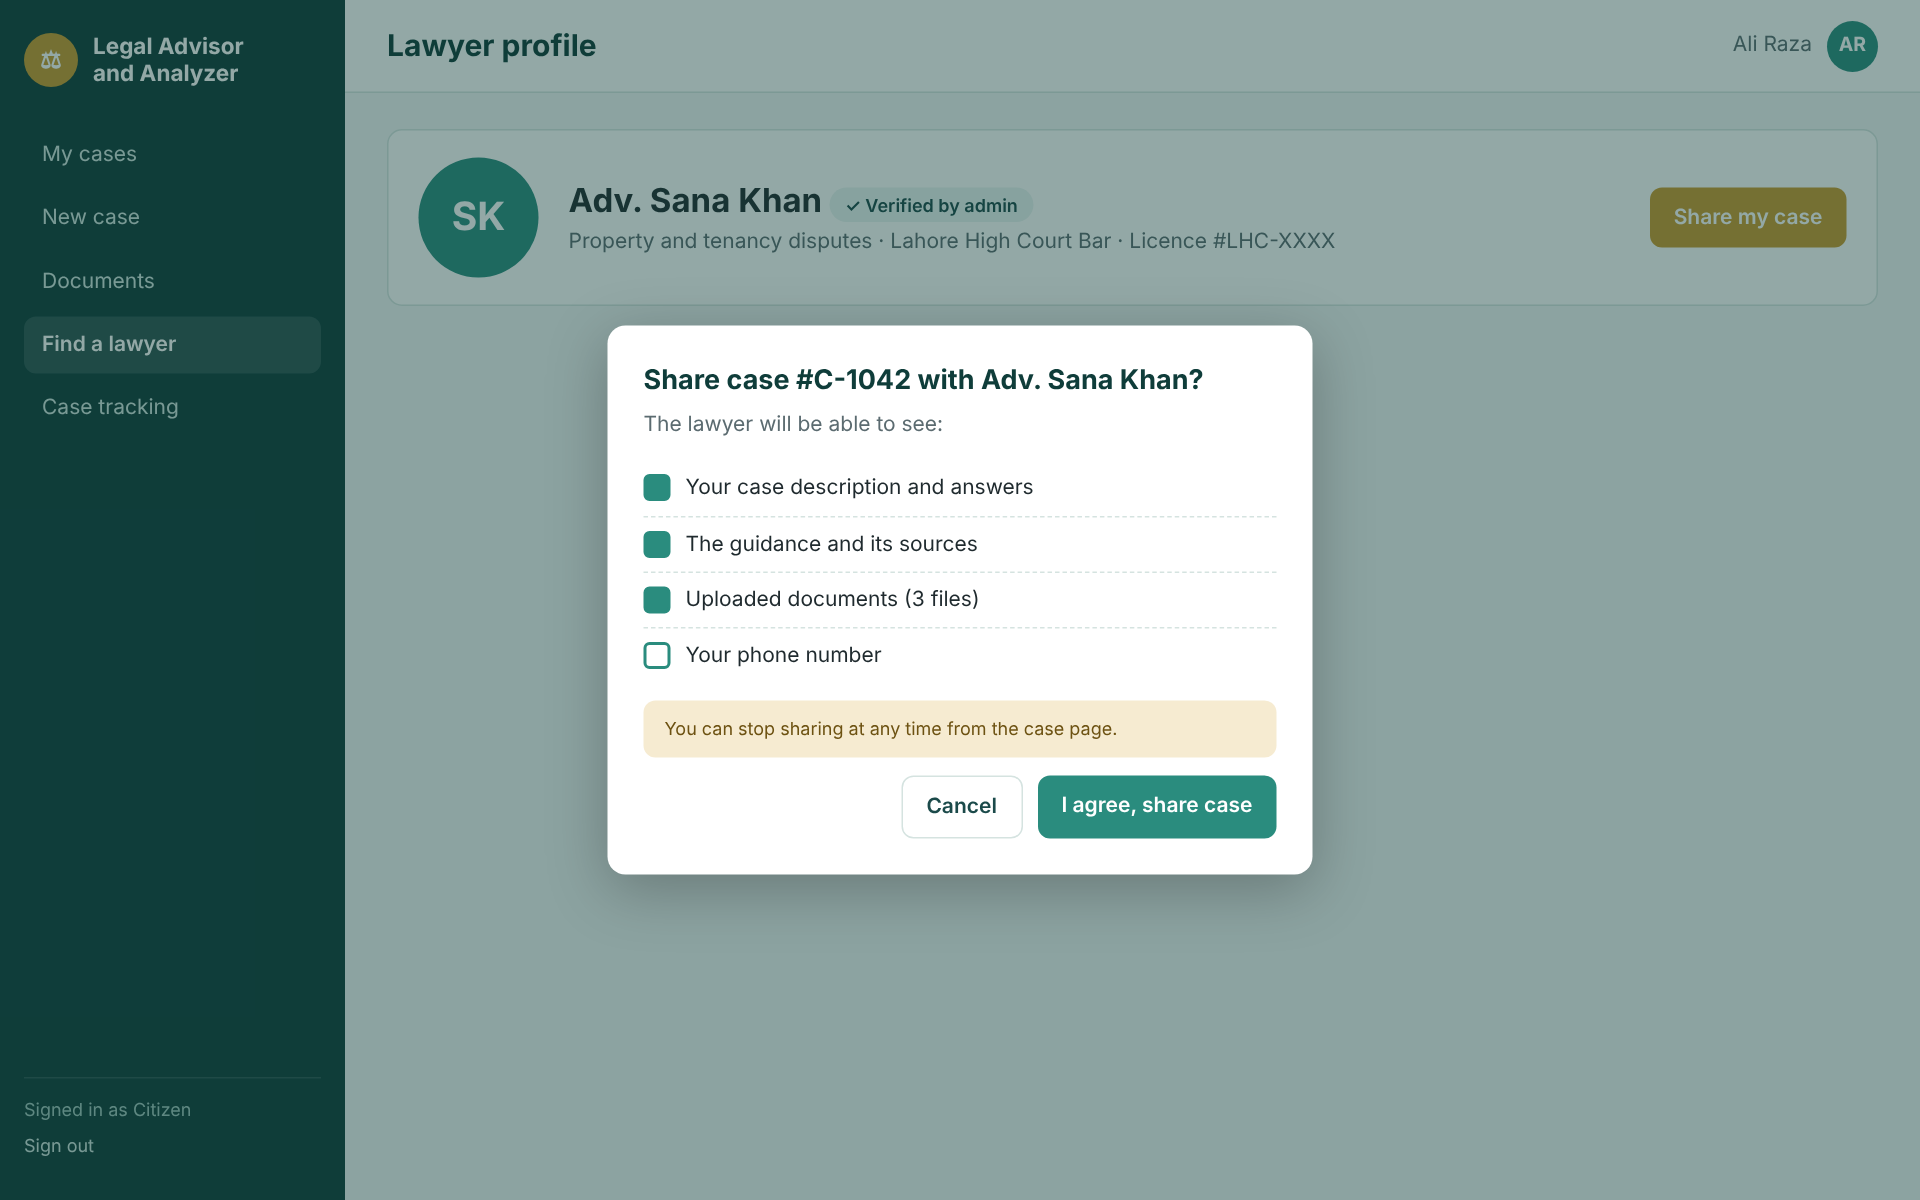
\includegraphics[width=\textwidth,height=0.62\textheight,keepaspectratio]{figures/screens/08_profile.png}
\caption{Lawyer profile header and consent dialog before sharing a case}\label{fig:3.21}
\end{figure}

\begin{figure}[H]\centering
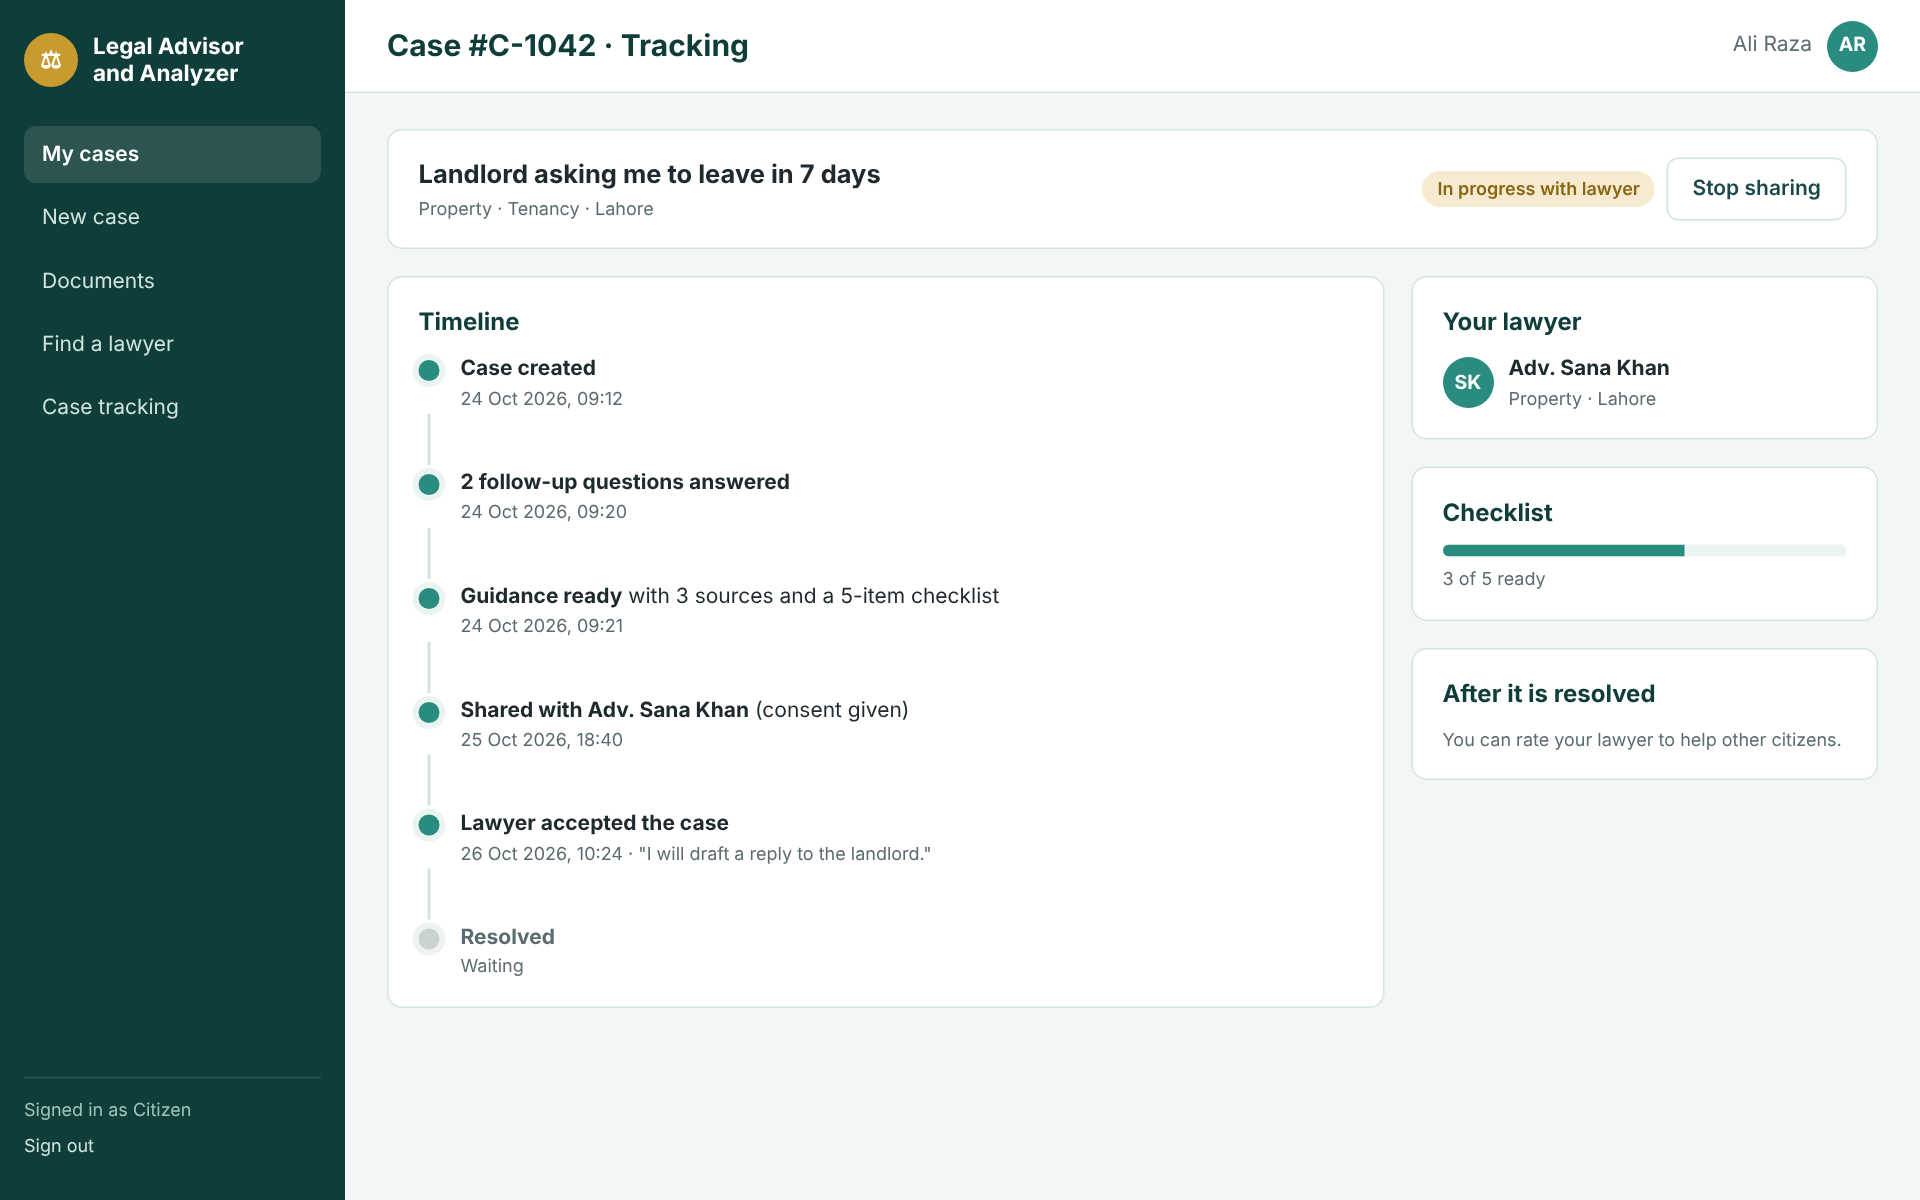
\includegraphics[width=\textwidth,height=0.62\textheight,keepaspectratio]{figures/screens/09_tracking.png}
\caption{Case tracking timeline}\label{fig:3.22}
\end{figure}

\needspace{12\baselineskip}
\subsection{Lawyer Portal}

\begin{center}
\begin{tabular}{|L{1.85cm}|L{7.93cm}|L{2.25cm}|L{1.98cm}|}
\hline\headrow \thd{Screen} & \thd{Purpose and key elements} & \thd{Requirements} & \thd{Status} \\ \hline
Lawyer dashboard & Cards for new requests, active cases, completed consultations and rating; table of new consultation requests with Accept/Decline; form to post a status update. & LFR-06, LFR-07, LFR-10, LFR-12 & Prototyped (Figure~\ref{fig:3.23}) \\ \hline
Profile editor & Sections for headline, about, practice areas, experience entries, education, languages, fees and photo, with a live preview of the public page and the verification status. & LFR-03 to LFR-05 & To be prototyped \\ \hline
Shared case view & Read-only case summary, AI guidance with sources, documents and checklist, limited to consented items. & LFR-08 & To be prototyped \\ \hline
Consultation detail & Schedule, status controls (Scheduled, Completed), message thread with the user. & LFR-07, LFR-09, LFR-11 & To be prototyped \\ \hline
\end{tabular}
\end{center}

\begin{figure}[H]\centering
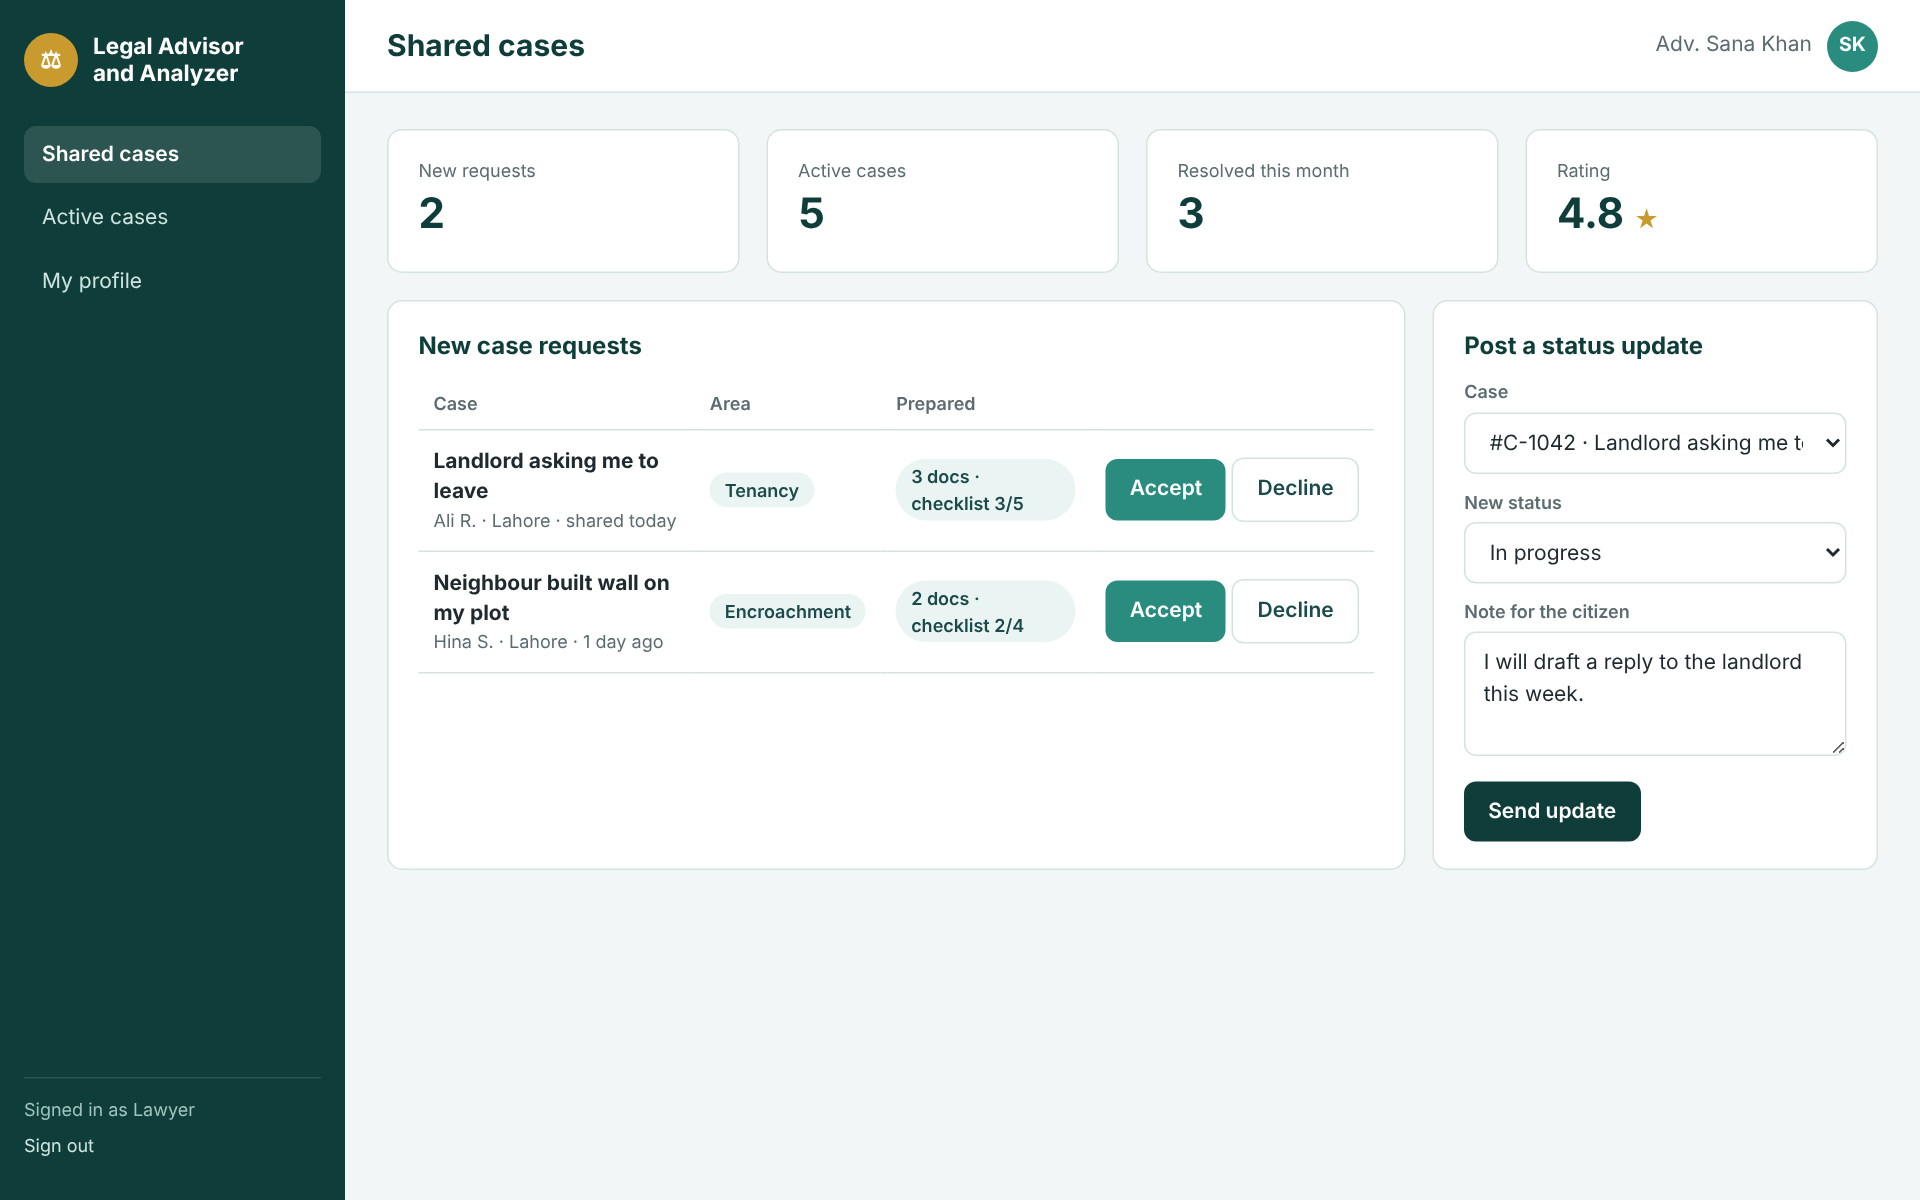
\includegraphics[width=\textwidth,height=0.62\textheight,keepaspectratio]{figures/screens/10_lawyer.png}
\caption{Lawyer portal dashboard}\label{fig:3.23}
\end{figure}

\needspace{12\baselineskip}
\subsection{Admin Portal}

\begin{center}
\begin{tabular}{|L{1.99cm}|L{7.46cm}|L{1.70cm}|L{2.86cm}|}
\hline\headrow \thd{Screen} & \thd{Purpose and key elements} & \thd{Requirements} & \thd{Status} \\ \hline
Admin dashboard & Platform statistics (users, verified lawyers, open cases, indexed sections); lawyer verification queue with Approve/Reject; knowledge-base summary per legal area. & AFR-02, AFR-05, AFR-08 & Prototyped (Figure~\ref{fig:3.24}) \\ \hline
User and lawyer management & Searchable table of accounts with role, status and actions (suspend, reactivate, remove). & AFR-03 & To be prototyped \\ \hline
Legal knowledge base & List of sources with type, year, area, status (processing, awaiting review, verified, retired); ``Add source''; chunk review panel. & AFR-05 to AFR-07 & Summary prototyped (Figure~\ref{fig:3.24}); full screen to be prototyped \\ \hline
Reports and moderation & Queue of reported profile items and reviews with keep/remove actions. & AFR-04 & To be prototyped \\ \hline
Audit log & Filterable list of administrative actions by date, admin and action type. & AFR-09 & To be prototyped \\ \hline
\end{tabular}
\end{center}

\begin{figure}[H]\centering
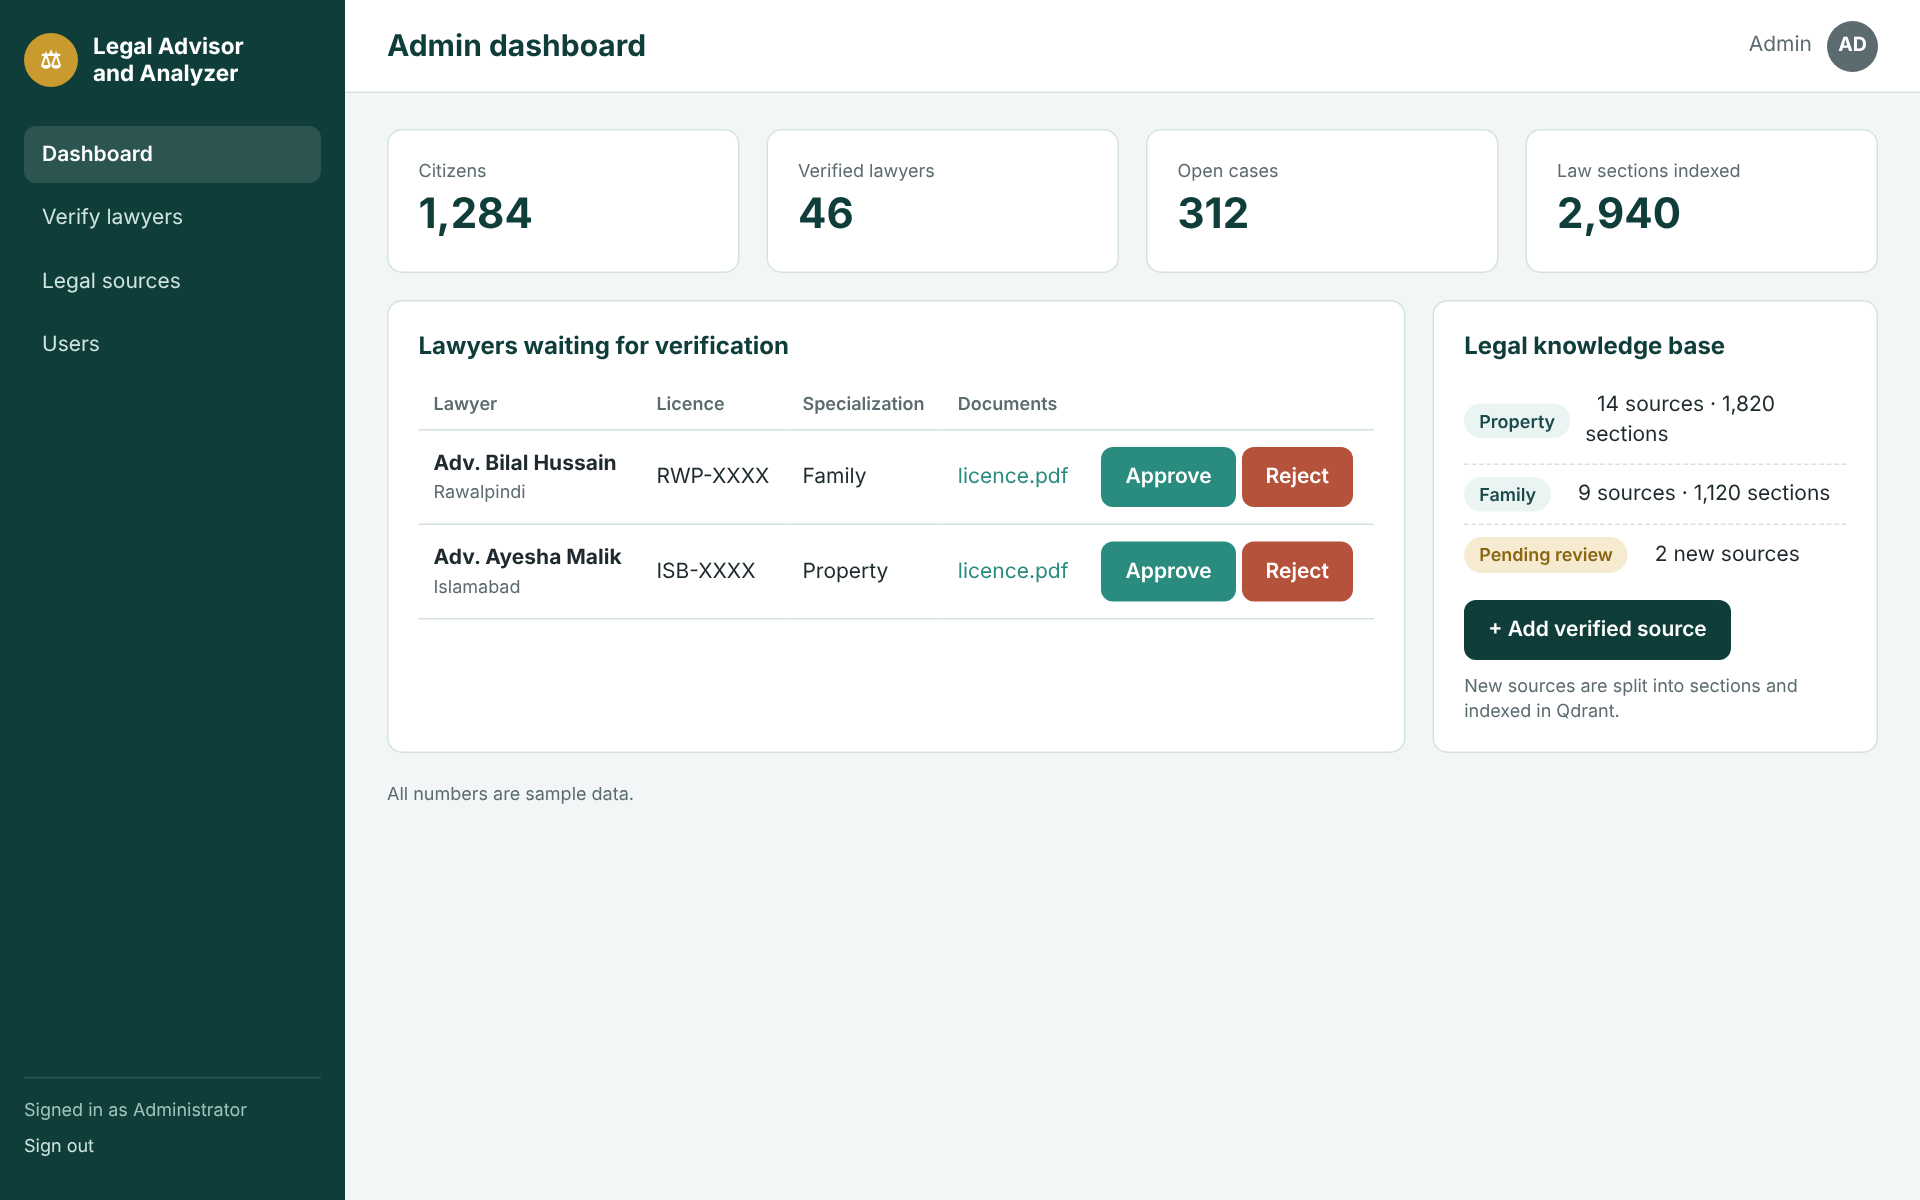
\includegraphics[width=\textwidth,height=0.62\textheight,keepaspectratio]{figures/screens/11_admin.png}
\caption{Admin portal dashboard}\label{fig:3.24}
\end{figure}

The prototypes use sample data (names, fees, statistics and example legal text) for illustration only. They reflect the planned behaviour of the system and do not represent implemented functionality.
